\documentclass[12pt]{report}

\usepackage{kotex}
\usepackage{amsmath}
\usepackage{amsfonts}
\usepackage{amssymb}
\usepackage{amsthm}
\usepackage{mathtools}
\usepackage{mathrsfs}
\usepackage{titlesec}
\usepackage{chngcntr}
\usepackage{bookmark}
\usepackage{ifthen}
\usepackage{import}
\usepackage[utf8]{inputenc}
\usepackage[a4paper]{geometry}
\geometry{
    top = 20mm,
    bottom = 20mm,
    left = 20mm,
    right = 20mm
}

% font styles
\usepackage{palatino}
\renewcommand{\sfdefault}{ppl}

% Changing counters
\usepackage{chngcntr}
\counterwithin*{footnote}{section}

% For styling enumerate
\usepackage{enumitem}
\setlist[enumerate,1]{label={(\arabic*)}}

% Line spacing
\usepackage[nodisplayskipstretch]{setspace}
\linespread{1.25}

\titleformat{\section}
{\normalfont\large\bfseries}{\thesection}{0em}{}

\setlength{\parindent}{0pt}

% Hyperlinks
\usepackage{hyperref}
\hypersetup{
    colorlinks=true,
    linkcolor=blue,
    bookmarks=true,
    unicode=true,
    urlcolor=blue
}

% Define colors
\usepackage{xcolor}

% Boxes
\usepackage{tikz}
\usepackage{tikz-cd}

% Skips between paragraph
\usepackage{parskip}
\setlength{\parskip}{8pt}

\renewcommand{\chaptername}{Part}
\renewcommand{\thechapter}{\Roman{chapter}}

\newcommand{\ds}{\displaystyle}

\newcommand{\mf}[1]{\mathfrak{#1}}
\newcommand{\mc}[1]{\mathcal{#1}}
\newcommand{\bb}[1]{\mathbb{#1}}
\renewcommand{\bf}[1]{\mathbf{#1}}

\newcommand{\inv}{^{-1}}
\newcommand{\adj}{\text{*}}
\newcommand{\cross}{^\times}
\newcommand{\bs}{\setminus}
\newcommand{\nsub}{\unlhd}
\newcommand{\pnsub}{\lhd}

\newcommand{\norm}[1]{\left\lVert #1 \right\rVert}
\newcommand{\abs}[1]{\left| #1 \right|}
\newcommand{\paren}[1]{\left( #1 \right)}
\newcommand{\seq}[1]{\left\{ #1 \right\}}
\renewcommand{\span}[1]{\left\langle #1 \right\rangle}
\renewcommand{\bar}[1]{\overline{#1 \vphantom{l}}}
\newcommand{\ind}[2]{\left(#1 : #2\right)}
\newcommand{\lcm}{{\rm lcm}}

\newcommand{\ra}{\rightarrow}
\newcommand{\imp}{\implies}
\newcommand{\mimp}{\(\implies\)}
\newcommand{\mimpd}{\(\impliedby\)}
\newcommand{\miff}{\!\!\(\iff\)}
\newcommand{\mast}{\(\ast\)}
\newcommand{\mstar}{\(\star\)}

\newcommand{\N}{\mathbb{N}}
\newcommand{\Z}{\mathbb{Z}}
\newcommand{\Q}{\mathbb{Q}}
\newcommand{\R}{\mathbb{R}}
\newcommand{\C}{\mathbb{C}}

\DeclareMathOperator{\im}{im}
\DeclareMathOperator{\ch}{char}
\DeclareMathOperator{\End}{End}
\DeclareMathOperator{\quotient}{/}
\newcommand{\irr}{\mathrm{irr}}
\newcommand{\GF}{\mathrm{GF}}

\let\oldexists\exists
\renewcommand{\exists}{\oldexists\,}

\let\oldtilde\tilde
\renewcommand{\tilde}[1]{\widetilde{#1}}

\newcommand{\defn}[1]{%
    \ifthenelse{\equal{#1}{.}}
    {\textbf{\sffamily Definition.}}%
    {\textbf{\sffamily Definition #1.}}%
}

\newcommand{\thm}[1]{%
    \ifthenelse{\equal{#1}{.}}
    {\textbf{\sffamily Theorem.}}%
    {\textbf{\sffamily Theorem #1.}}%
}

\newcommand{\prop}[1]{%
    \ifthenelse{\equal{#1}{.}}
    {\textbf{\sffamily Proposition.}}%
    {\textbf{\sffamily Proposition #1.}}%
}

\newcommand{\ex}[1]{%
    \ifthenelse{\equal{#1}{.}}
    {\textbf{\sffamily Example.}}%
    {\textbf{\sffamily Example #1.}}%
}

\newcommand{\prob}[1]{%
    \ifthenelse{\equal{#1}{.}}
    {\textbf{\sffamily Problem.}}%
    {\textbf{\sffamily Problem #1}}%
}

\newcommand{\lemma}[1]{%
    \ifthenelse{\equal{#1}{.}}
    {\textbf{\sffamily Lemma.}}%
    {\textbf{\sffamily Lemma #1.}}%
}

\newcommand{\cor}[1]{%
    \ifthenelse{\equal{#1}{.}}
    {\textbf{\sffamily Corollary.}}%
    {\textbf{\sffamily Corollary #1.}}%
}

\newcommand{\recall}{\textbf{\sffamily Recall.\;}}
\newcommand{\rmk}{\textbf{\sffamily Remark.\;}}
\newcommand{\pf}{\textit{\sffamily Proof.\;}}
\newcommand{\question}{\textbf{\sffamily Question.\;}}
\newcommand{\notation}{\textbf{\sffamily Notation.\;}}
\newcommand{\claim}{\textbf{Claim}}

\newcommand{\note}[1]{({\sffamily #1})}
\newcommand{\sref}[1]{{\sffamily #1}}

\newcounter{topic}
\setcounter{topic}{0}
\newcommand{\topic}[1]{
    \addtocounter{topic}{1}
    \vspace{15pt}
    \textbf{\large Section \thetopic.\, #1}
    \vspace{3pt}
    \hrule
    \vspace{10pt}
}


% overriding styles
\linespread{1.25}
\setlength{\parskip}{8pt}

\usepackage{palatino}
\renewcommand{\sfdefault}{ppl}

\title{\textbf{Modern Algebra II}}
\author{Sungchan Yi}
\date{Fall 2023}

\begin{document}

\maketitle

\setcounter{chapter}{5}

\chapter{Extension Fields}

\textbf{Topics for this semester}: Extension Fields, Galois Theory, Advanced Group Theory.

\setcounter{topic}{28}
\topic{Introduction to Extension Fields}

Examples of fields: \(\Z_p\), \(\Q\), \(\R\), \(\C\) and the field of quotients. We now introduce more examples. The idea is the following:

\recall Let \(R\) be a commutative ring with unity.\footnote{In this semester, \(R\) will almost always have a unity.} If \(M\) is a maximal ideal of \(R\), then \(R \quotient M\) is a field.

We will construct new examples from this proposition. For example, given a polynomial ring \(F[x]\) where \(F\) is a field, \(F[x] \quotient M\) is a field if \(M\) is a maximal ideal of \(F[x]\). Our task will be to describe \(M\), and then \(F[x] \quotient M\).

\recall \(M\) is a maximal ideal of \(F[x] \iff M = \span{p(x)}\), with \(p(x)\) irreducible. So \(F[x]\) is a principal ideal domain, i.e, all ideals of \(F[x]\) are principal (generated by a single element).

Thus if we set \(M = \span{p(x)}\) where \(p(x)\) is a irreducible polynomial, \(F[x] \quotient M\) would be a field.

\question Why do we call \(F[x] \quotient M\) an \textit{extension} field? Because \(F \hookrightarrow {F[x]} \quotient {\span{p(x)}}\).\footnote{\(a \in F[x]\), injective.}

\question Why do we consider extension fields?

Consider \(x^2 + 1 \in \R[x]\). This polynomial has no solutions in \(\R\), but we want a new field containing \(R[x]\) and also the \textit{roots} of \(x^2 + 1\). So we consider \(\R[x] \quotient \span{x^2 + 1}\).

\pagebreak

\defn. \note{Extension Field} Let \(F\) be a field. \(E\) is an \textbf{extension field} of \(F\) if \(E\) is a field and \(F \leq E\).

\ex. Tower of extension fields.
\begin{enumerate}
    \item \(\Q \leq \R \leq \C\).
    \item \(F \leq F(x) \leq F(x, y)\) where \(F(x) = \left\{\frac{f(x)}{g(x)} : f(x), g(x) \in F[x], g(x) \neq 0\right\}\).
\end{enumerate}

\recall \(\alpha\) is a \textbf{zero} of \(f(x) \in F[x]\) if there exists an \textit{extension field} \(E\) of \(F\) containing \(\alpha\), such that for the \textbf{evaluation homomorphism} \(\varphi_\alpha : F[x] \ra E\) defined as \(a \mapsto a\) (\(a \in F\)), \(x \mapsto \alpha\), we have \(\varphi_\alpha(f(x)) = 0\).

\thm. \note{Kronecker} \footnote{The book says that this is our basic goal.} Let \(f(x) \in F[x]\) be a nonconstant polynomial. Then there exists an extension field \(E\) and \(\alpha \in E\) such that \(f(\alpha) = 0\).

\pf Let \(f(x) = p_1(x)p_2(x)\cdots p_m(x)\) where \(p_i(x)\) are irreducible polynomials in \(F[x]\). We will show that for \(p(x) \in \{p_1(x), \dots, p_m(x)\}\), \(E = F[x] \quotient \span{p(x)}\) is the field we want, and \(\alpha = x + \span{p(x)}\) is a zero of \(f(x)\).

First, it is clear that \(E\) is an extension field of \(F\) since \(p(x)\) is irreducible, and the map \(\varphi: F \ra E\) defined as \(1 \mapsto 1 + \span{p(x)}\) is injective. Next, to show that \(\alpha\) is a zero of \(f(x)\), it is enough to show that \(\alpha\) is a zero of \(p(x)\). If \(p(x) = \sum_{i=0}^d a_ix^i\), then
\[
    \varphi_\alpha(p(x)) = \sum_{i=0}^d a_i \paren{x + \span{p(x)}}^i = \sum_{i=0}^d a_ix^i + \span{p(x)} = p(x) + \span{p(x)} = 0 + \span{p(x)},
\]
so \(\alpha\) is a zero. \qed

If \(f(x)\) does not have a zero in \(F\), we can also think of \(f(x)\) as an irreducible polynomial in \(F[x]\). By Kronecker's theorem, we can extend \(F\) to a field \(E\) where \(f(x)\) has a zero. An example would be \(f(x) = x^2 + 1 \in \R[x]\), where we take \(\alpha = x + \span{x^2 + 1} \in F[x] \quotient \span{x^2 + 1}\).

\defn. Let \(E\) be an extension field of \(F\).
\begin{enumerate}
    \item \(\alpha \in E\) is \textbf{algebraic} over \(F\) if there exists \(f(x) \in F[x]\) such that \(f(\alpha) = 0\).
    \item Otherwise, \(\alpha \in E\) is called \textbf{transcendental} over \(F\).
\end{enumerate}

When we don't specify the field \(F\), we think of it as \(\Q\).

\defn. For \(\alpha \in \C\),
\begin{enumerate}
    \item \(\alpha\) is \textbf{algebraic} if \(\alpha\) is algebraic over \(\Q\).
    \item \(\alpha\) is \textbf{transcendental} if \(\alpha\) is transcendental over \(\Q\).
\end{enumerate}

\thm. Let \(E\) be an extension field of \(F\) and \(\alpha \in E\). Then \(\varphi_\alpha : F[x] \ra E\) is bijective if and only if \(\alpha\) is transcendental over \(F\).

\pf \(\alpha\) is algebraic \(\iff \exists f(x) \in F[x]\) such that \(\varphi_\alpha(f(x)) = 0 \iff \varphi_\alpha\) is not bijective.\\
(\(\ker \varphi_\alpha\) is not trivial, then it is an ideal and \(F[x]\) is a PID...) \qed

\section*{Irreducible Polynomials for \(\alpha\) over \(F\)}

\thm. Let \(E\) be an extension field of \(F\) and \(\alpha \in E\) be algebraic over \(F\).\footnote{This hypothesis makes sense because of Kronecker's theorem.}
\begin{enumerate}
    \item There exists a unique \textit{monic irreducible} polynomial \(p(x) \in F[x]\) such that \(p(\alpha) = 0\).
    \item If \(f(\alpha) = 0\) for \(f(x) \in F[x]\), then \(f(x) \in \span{p(x)}\).
\end{enumerate}

\pf Consider the evaluation homomorphism \(\varphi_\alpha : F[x] \ra E\). Since \(\alpha\) is algebraic, \(\ker \varphi_\alpha = \span{p(x)}\) for some monic polynomial \(p(x) \in F[x]\). We must show that \(p(x)\) is irreducible.

\note{1} If \(p(x)\) is reducible, choose nonconstant polynomials \(r(x), s(x) \in F[x]\) such that \(p(x) = r(x)s(x)\). Then \(r(\alpha) = 0\) or \(s(\alpha) = 0\). Without loss of generality, if \(r(\alpha) = 0\), \(r(x) \in \span{p(x)}\) which is a contradiction.

\note{2} If \(f(\alpha) = 0\), then \(f(x) \in \ker\varphi_\alpha = \span{p(x)}\). \qed

Since an algebraic \(\alpha \in E\) determines a unique monic irreducible polynomial, we have the following definition.

\defn. Let \(E\) be an extension field of \(F\) and \(\alpha \in E\) be algebraic over \(F\).
\begin{enumerate}
    \item Then the unique irreducible monic polynomial \(p(x) \in F[x]\) is denoted by \(\irr(\alpha, F)\).
    \item \(\deg (\alpha, F) = \deg \irr(\alpha, F)\).
\end{enumerate}

Our conclusion today is that for any algebraic \(\alpha \in E\) over \(F\), there exists a unique monic irreducible polynomial \(\irr(\alpha, F)\), and any other polynomial in \(F[x]\) having \(\alpha\) as a zero will have \(\irr(\alpha, F)\) as a factor.

\(E\) was an arbitrary extension field of \(F\) containing \(\alpha\). Our intuition is that \(F[x] \quotient \irr(\alpha, F)\) would be the smallest extension field containing \(\alpha\). We will prove this next time, and compare it with \(F\) and describe it using \(F\).

\pagebreak

\section*{Simple Extensions}

We want to study properties of extension fields, so we start from \textit{simple extensions}, as we started from \textit{simple groups} in group theory.

Let \(F\) be a field, \(E\) be an extension field of \(F\) and \(\alpha \in E\).

Naively, what do we mean by \textit{simple}? We denote simple extensions as \(F(\alpha)\), which is an extension field of \(F\) in \(E\) that satisfies: (i) \(\alpha \in F(\alpha)\), (ii) it is the smallest field containing \(F\) and \(\alpha\). So adding a \textit{single element} \(\alpha\) to \(F\) will generate the whole field \(F(\alpha)\).

We have two cases of simple extensions, whether if \(\alpha \in E\) is algebraic or not.

\begin{itemize}
    \item If \(\alpha\) is \textit{algebraic} over \(F\), for the evaluation homomorphism \(\varphi_\alpha : F[x] \ra E\), we have \(\ker \varphi_\alpha = \span{\irr(\alpha, F)}\). By the first isomorphism theorem, we have \(F[x] \quotient \ker\varphi_\alpha \simeq \im \varphi_\alpha\). Since \(\varphi_\alpha\) maps \(a\) to \(a\) and \(x\) to \(\alpha\), any field containing \(F\) and \(\alpha\) must contain \(\im \varphi_\alpha\). We see that \(\im \varphi_\alpha = F(\alpha)\).

    \item If \(\alpha\) is \textit{transcendental} over \(F\), \(\varphi_\alpha : F[x] \ra E\) is an injective map. So \(\ker \varphi_\alpha = 0\), and \(F[x] \simeq \im\varphi_\alpha\), which is not a field. But it is an \textit{integral domain}! So we can consider the \textit{field of quotients}, which is the smallest field containing \(\im \varphi_\alpha\).\footnote{Up to isomorphism.} Therefore,
    \[
        F(\alpha) = \left\{\frac{f(\alpha)}{g(\alpha)} : g(x) \neq 0, f(x), g(x) \in F[x]\right\} \simeq F(x).
    \]
\end{itemize}

\defn. \note{Simple Extension} For \(\alpha \in E\), \(F(\alpha)\) is called a \textbf{simple extension} of \(F\).
\begin{enumerate}
    \item If \(\alpha\) is algebraic over \(F\), then \(F(\alpha) = \im \varphi_\alpha\).
    \item If \(\alpha\) is transcendental over \(F\), then \(F(\alpha)\) is the field of quotients of \(\im \varphi_\alpha\).
\end{enumerate}

Now we would like to describe \(F(\alpha)\) when \(\alpha\) is algebraic over \(F\).

\thm. Let \(\alpha\) be algebraic over \(F\) and \(E = F(\alpha)\). Let \(n = \deg(\alpha, F)\). Then \(E\) is an \(n\)-dimensional vector space over \(F\) with basis \(\mf{B} = \{1, \alpha, \alpha^2, \dots, \alpha^{n-1}\}\).

\pf We will show that \(\mf{B}\) is a basis.
\begin{itemize}
    \item \note{\(\mf{B}\) spans \(E\)} \(E = \im \varphi_\alpha\). Then \(\beta \in E\) has the form \(\beta = g(\alpha)\) for \(g(x) \in F[x]\). By the division algorithm, we can choose \(q(x), r(x) \in F[x]\) so that \(g(x) = \irr(\alpha, F) q(x) + r(x)\) and \(\deg r < n\). So \(\beta = g(\alpha) = r(\alpha) \in \span{\mf{B}}\).
    \item \note{\(\mf{B}\) is linearly independent} Let \(g(x), h(x) \in F[x]\) with \(\deg g, \deg h < n\). Suppose that \(g(\alpha) = h(\alpha)\). Then \((g-h)(x) \in \ker \varphi_\alpha\), which is a contradiction since \(\deg (g-h) < n\). \qed
\end{itemize}

\pagebreak

\ex. We know \(\R \leq \C\). \(\C = \R(i) = \R \oplus i\R\). So \(\C\) is a 2-dimensional \(\R\)-vector space with basis \(\{1, i\}\). Also, \(\irr(i, \R) = x^2 + 1\) so we could also write \(\C \simeq \R[x] \quotient \span{x^2 + 1}\).

\ex. Let \(p(x) = x^2 + x + 1 \in \Z_2[x]\). Then \(\Z_2[x] \quotient \span{p(x)}\) is a field, since \(p(x)\) is irreducible.\footnote{\(p(0) = p(1) = 1\) so it cannot have a factor.} Let \(\alpha\) be a zero of \(p(x)\). Then \(\Z_2(\alpha) = \span{1, \alpha} = \left\{0, 1, \alpha, 1 + \alpha\right\}\). Now we can define operations on this field. Addition is easy, and we can check that \(\alpha\inv = \alpha + 1\).

\setcounter{topic}{30}
\topic{Algebraic Extensions}

Our next simplest example is finite extensions. We will show that finitely many simple extensions leads to finite extensions.

\defn. \note{Finite Extension}
\begin{enumerate}
    \item Let \(E\) be an extension field of \(F\). If \(E\) is a finite dimensional \(F\)-vector space, then \(E\) is called a \textbf{finite extension} over \(F\).

    \item If \(E\) is a finite extension and \(E\) is a \(n\)-dimensional \(F\)-vector space, then \(E\) is a finite extension of degree \(n\) and we denote \([E : F] = n\).
\end{enumerate}

\cor. Let \(\alpha \in E\) be algebraic over \(F\). Then \(F(\alpha)\) is a finite extension with \([F(\alpha) : F] = \deg(\alpha, F)\).

We have just shown that simple algebraic extensions are finite extensions. The converse is not true.

\smallskip

\defn. \note{Algebraic Extension} Let \(E\) be an extension field of \(F\). \(E\) is an \textbf{algebraic extension} of \(F\) if all elements in \(E\) are algebraic over \(F\).

\begin{center}
    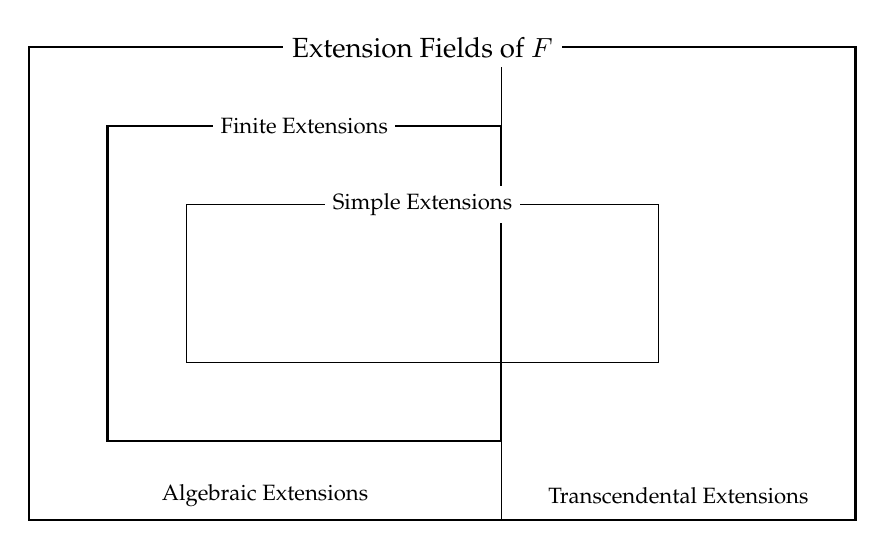
\begin{tikzpicture}
        \draw[thick] (0, 0) rectangle (10.5, 6);
        \draw (6, 0) -- (6, 6);
        \draw (2, 2) rectangle (8, 4);
        \draw[thick] (1, 1) rectangle (6, 5);
        \node[fill=white] at (5, 6) {Extension Fields of \(F\)};
        \node[fill=white, scale=0.8] at (3, 0.3) {Algebraic Extensions};
        \node[fill=white, scale=0.8] at (8.25, 0.3) {Transcendental Extensions};
        \node[fill=white, scale=0.8] at (3.5, 5) {Finite Extensions};
        \node[fill=white, scale=0.8] at (5, 4) {Simple Extensions};
    \end{tikzpicture}
\end{center}

\thm. Every finite extension is an algebraic extension.

\pf Let \(E\) be a finite extension of degree \(n\) over \(F\). Take \(\alpha \in E\). Then \(\{1, \alpha, \dots, \alpha^{n-1}, \alpha^n\}\) is linearly dependent over \(F\).\footnote{Recall from linear algebra: if \(\dim_F E = n\), then any subset of \(E\) with more than \(n\) elements is linearly dependent over \(F\).} Then we can choose \(b_0, \dots, b_n \in F\) such that
\begin{center}
    \(b_0 + b_1 \alpha + \cdots + b_n\alpha^n = 0\) and \(b_i \neq 0\) for some \(i\).
\end{center}
Equivalently, if we set \(f(x) = b_0 + b_1 x + \cdots + b_n x^n \in F[x]\), then \(f(x) \neq 0\) and \(f(\alpha) = 0\). Thus any element \(\alpha \in E\) is algebraic. \qed

\cor. If \(\alpha \in E\) is algebraic over \(F\) then \(F(\alpha)\) is an algebraic extension.

\thm. Let \(E\) be a finite extension over \(F\), and \(K\) be a finite extension over \(E\). Then
\[
    [K: F] = [K : E] [E : F].
\]

\pf Set \(m = [K : E]\), \(n = [E : F]\). Let \(\{\alpha_1, \dots, \alpha_n\}\) be an \(F\)-basis of \(E\) and \(\{\beta_1, \dots, \beta_m\}\) be an \(E\)-basis of \(K\). Now we show that
\[
    \mf{B} = \{\alpha_i \beta_j : 1 \leq i \leq n,\, 1 \leq j \leq m\}
\]
is an \(F\)-basis of \(K\).
\begin{itemize}
    \item (\(\mf{B}\) spans \(K\) over \(F\)) Check by yourself.
    \item (\(\mf{B}\) is linearly independent) Suppose for \(c_{ij} \in F\), we have \(\sum_{i, j} c_{ij}\alpha_i\beta_j = 0\). Then we can write
    \[
        \sum_{i, j} c_{ij}\alpha_i\beta_j = \sum_{j}\paren{\sum_{i} c_{ij}\alpha_i}\beta_j = 0.
    \]
    Since \(\beta_j\) are linearly independent, \(\sum_i c_{ij} \alpha_i = 0\) for all \(j\). In the same way, linear independence of \(\alpha_i\) gives \(c_{ij} = 0\) for all \(i, j\). \qed
\end{itemize}

Let \(\tilde{F}\) be an extension field of \(F\) and let \(\alpha \in \tilde{F}\) be algebraic. Then \(E = F(\alpha)\) is a simple, finite extension. Take another element \(\beta \in E\), that is algebraic in an extension field \(\tilde{E}\). Then to describe \(E(\beta)\), we can split the field into two simple extensions,
\[
    [E(\beta) : F] = \overbrace{[E(\beta) : E]}^{\text{simple}} \overbrace{[F(\alpha) : F]}^{\text{simple}}.
\]
and inspect each simple extension.

\cor. Let \(F_{i+1}\) be a finite extension field over \(F_i\) for \(i = 1, \dots, r - 1\). Then \(F_r\) is a finite extension of \(F_1\) and
\[
    [F_r : F_1] = [F_r : F_{r - 1}] [F_{r - 1} : F_{r - 2}] \cdots [F_2 : F_1].
\]

\cor. Let \(\alpha \in E\) be algebraic over \(F\). If \(\beta \in F(\alpha)\), then \(\deg(\beta, F) \mid \deg(\alpha, F)\).

\pf \(F \subset F(\alpha)\), \(\beta \in F(\alpha)\), so \(F(\beta) \subset F(\alpha)\) since \(F(\beta)\) is the smallest subfield. Thus \(F(\alpha)\) is an extension field of \(F(\beta)\). Also, from \(\beta \in F(\alpha)\), \(\beta\) is algebraic over \(F\). Therefore,
\[
    \deg(\alpha, F) = [F(\alpha) : F] = [F(\alpha) : F(\beta)] [F(\beta) : F] = [F(\alpha) : F(\beta)] \cdot \deg(\beta, F).
\]
\qed

\rmk Any extension field of \(F\) is an \(F\)-vector space.

\ex. \(x^3 - 2\) does not have a zero in \(\Q(\sqrt{2})\).

\pf Note that \(x^3 - 2\) is irreducible.\footnote{If reducible, it should have a linear factor, but \(\sqrt[3]{2} \notin \Q\).} Let \(\beta\) be a zero of \(x^3 - 2 \in \Q[x]\). Then \(\irr(\beta, \Q) = x^3 - 2\), so \(\deg(\beta, \Q) = [\Q(\beta) : \Q] = 3\). But since \(\irr(\sqrt{2}, \Q) = x^2 - 2\), \([\Q(\sqrt{2}) : \Q] = 2\). Thus \(\beta \notin \Q(\sqrt{2})\) since \(3 \nmid 2\). \qed

\ex. By definition, \(\Q \leq \Q(\sqrt{2}) \leq \Q(\sqrt{2}, \sqrt{3})\). But is \(\Q(\sqrt{2}, \sqrt{3})\) simple?

\pf Consider \(E = \Q(\sqrt{2} + \sqrt{3})\). Then \(\frac{1}{\sqrt{2} + \sqrt{3}} = \sqrt{3} - \sqrt{2} \in E\). We can easily see that
\[
    \sqrt{3} = \frac{1}{2}(\sqrt{3} + \sqrt{2}) + \frac{1}{2}(\sqrt{3} - \sqrt{2}) \in E, \qquad \sqrt{2} = \frac{1}{2}(\sqrt{3} + \sqrt{2}) - \frac{1}{2}(\sqrt{3} - \sqrt{2}) \in E.
\]
Thus \(\sqrt{2}, \sqrt{3} \in E\) and \(\Q(\sqrt{2}, \sqrt{3}) \subset E\). Conversely, \(\sqrt{2} + \sqrt{3} \in \Q(\sqrt{2}, \sqrt{3})\), so \(E \subset \Q(\sqrt{2}, \sqrt{3})\). We can conclude that \(\Q(\sqrt{2}, \sqrt{3}) = \Q(\sqrt{2} + \sqrt{3})\) is a simple extension. \qed

So \textit{adjoining} another element to a simple extension might still be a simple extension.\footnote{What is \textit{not} a simple extension? This is a hard question.}

\pagebreak

\thm. Let \(E\) be an algebraic extension of \(F\). Then \(E\) is a finite extension if and only if there exists finitely many \(\alpha_1, \dots, \alpha_n \in E\) such that \(E = F(\alpha_1, \dots, \alpha_n)\).

\pf \note{\mimp} Take \(\alpha_1 \in E \bs F\) and consider \(F(\alpha_1)\). If \(F(\alpha_1) \neq E\), take \(\alpha_2 \in E \bs F(\alpha_1)\) and consider \(F(\alpha_1, \alpha_2)\). Repeat the process until \(E = F(\alpha_1, \dots, \alpha_n)\). This process terminates because \(E\) is a finite extension and adjoining \(\alpha_i\) is an extension of degree greater than \(1\).

\note{\mimpd} Suppose that \(E = F(\alpha_1, \dots, \alpha_n)\). All \(\alpha_i\) are algebraic over \(F\) since \(E\) is an algebraic extension of \(F\). So \(F(\alpha)\) is a simple algebraic extension of \(F\), and \(F(\alpha_1, \dots, \alpha_{i})\) is a simple algebraic extension of \(F(\alpha_1, \dots, \alpha_{i - 1})\) for \(i = 2, \dots, n\). Since simple algebraic extensions are finite extensions, \([F(\alpha_1, \dots, \alpha_n) : F]\) can be decomposed into a finite product. Thus \(E\) is a finite extension. \qed

Generally, it is very hard to find an element \(\alpha \in E\) such that \(E = F(\alpha) = F(\alpha_1, \dots, \alpha_n)\). So using each \(\alpha_i\) as a building block is a lot more effective.

\pagebreak

\section*{Algebraic Closures}

\defn. \note{Algebraic Closure} Let \(E\) be an extension field of \(F\).
\begin{center}
    \(\bar{F}_E = \{\alpha \in E : \alpha \text{ is algebraic over } F\}\)
\end{center}
is called the \textbf{algebraic closure of \(F\) in \(E\)}.

\prop. \(\bar{F}_E\) is a field, and \(F \leq \bar{F}_E\).

\pf It is enough to show that \(\alpha \pm \beta\), \(\alpha \beta\), \(\alpha / \beta\) (\(\beta \neq 0\)) are in \(\bar{F}_E\) for all \(\alpha, \beta \in \bar{F}_E\). Associativity, commutativity and the distributive property directly follows since \(E\) is a field.

Consider \(F(\alpha, \beta) \subset E\). \(\alpha, \beta\) are algebraic over \(F\), so \(F(\alpha, \beta)\) is a finite extension and also an algebraic extension. Thus all elements of \(F(\alpha, \beta)\) are algebraic over \(F\), and \(F(\alpha, \beta) \subset \bar{F}_E\). The result directly follows. \qed

\defn. \note{Algebraically Closed Field}
\begin{enumerate}
    \item A field \(F\) is \textbf{algebraically closed} if every non-constant polynomial in \(F[x]\) has a zero in \(F\).
    \item \(\bar{F}\) is the \textbf{algebraic closure of \(F\)}, which is an algebraic extension field of \(F\) such that every non-constant polynomial in \(\bar{F}[x]\) has a zero in \(\bar{F}\).
\end{enumerate}

\(\bar{F}\) is a field containing all zeros of \(F[x]\). Does it actually exist? We need Zorn's lemma to construct the algebraic closure.

\defn. \note{Partially Ordered Set} \((S, \leq)\) is a \textbf{partially ordered set} if
\begin{enumerate}
    \item (Reflexive) \(\forall s \in S\), \(s \leq s\).
    \item (Anti-symmetric) \(\forall a, b \in S\), if \(a \leq b\) and \(b \leq a\), then \(a = b\).
    \item (Transitive) \(\forall a, b, c \in S\), if \(a \leq b\) and \(b \leq c\), then \(a \leq c\).
\end{enumerate}

\defn. \note{Chain} Let \(S\) be a partially ordered set. \(T \subset S\) is a \textbf{chain} if
\begin{center}
    \(\forall a, b \in T\), \(a \leq b\) or \(b \leq a\).
\end{center}
i.e, we can compare any two elements of \(T\).

\lemma. \note{Zorn} Let \(S\) be a partially ordered set. If every chain \(T \subset S\) has an upper bound in \(S\), then \(S\) has at least one maximal element.

\pf Equivalent to the Axiom of Choice. \qed

To use Zorn's lemma, we need to define a partially ordered set, and show that every chain has an upper bound. Finally, we should check if the maximal element of \(S\) can indeed be called the algebraic closure.

\thm. Every field has an algebraic closure \(\bar{F}\).

\pf Let \(S\) be the set of all algebraic extensions of \(F\).\footnote{\textit{Is \(S\) actually a set? Does it actually exist?}} We define a relation \(\leq\) as the following. For \(E_i, E_j \in S\), \(E_i \leq E_j \iff E_i \subset E_j\). It can be checked that \(S\) is a partially ordered set.

Let \(T = \{E_j : j \in J\}\) be a chain in \(S\), and take \(W = \bigcup_{E \in T} E\). \(W\) is an upper bound by definition, so we must show that \(W \in S\). We will show that (i) \(W\) is a field, and (ii) \(W\) is an algebraic extension field of \(F\).

\note{i} Suppose that \(\alpha \subset E_i\), \(\beta \subset E_j\) where \(E_i \subset E_j\) in \(T\). Then \(\alpha, \beta \in E_j\), where \(E_j\) is a field. So \(\alpha \pm \beta\), \(\alpha\beta\), \(\alpha / \beta \in E_j \subset W\). \(W\) is a field.

\note{ii} Let \(\alpha \in W\). Then \(\alpha \in E\) for some \(E \in T\). \(E\) is an algebraic extension of \(F\), so \(\alpha\) is algebraic over \(F\), and thus \(W\) is an algebraic extension of \(F\).

By Zorn's lemma, take a maximal element \(\bar{F}\) of \(S\). We show that \(\bar{F}\) is algebraically closed.

Suppose not. Then there exists a irreducible polynomial in \(\bar{F}[x]\) having degree greater than 1. Let \(\alpha\) be a zero of \(f(x)\). \(\bar{F}(\alpha)\) is an algebraic extension of \(F\), so \(\bar{F} < \bar{F}(\alpha) \in S\), contradicting that \(\bar{F}\) is maximal. \qed

\pagebreak

\topic{Geometric Constructions}

We have a straightedge and a compass.\footnote{A \textit{ruler} has marks on it!} A straightedge is used to draw or extend straight lines, and a compass is used to draw circles or copy lengths. We are also given a line segment, as a unit length.

\defn. \note{Constructible Real Number} A real number \(\alpha\) is \textbf{constructible} if we can construct a line segment of length \(\abs{\alpha}\) in a finite number of steps from a given segment of unit length by using a straightedge and a compass.

It is easy to see that with the given unit length as \(1\), any integer is constructible. The following theorem shows that constructible real numbers form a field.

\thm. Let \(\alpha, \beta\) be constructible real numbers. Then
\[
    \alpha \pm \beta, \quad \alpha\beta, \quad \alpha / \beta\;\; (\beta \neq 0)
\]
are constructible.

\pf We are given lengths \(\alpha\), \(\beta\) and \(1\). \(\alpha \pm \beta\) is very simple.

As for constructing \(\alpha \beta\), refer to the diagram on the left. Start with given lengths \(OA = \alpha\) and \(OB = \beta\), with an arbitrary angle. Pick a point \(P\) with \(OP = 1\) on the line \(OB\). Then construct a line from \(B\) that is parallel to \(AP\). Let \(Q\) be the intersection of \(OA\) with this line. Then the triangles \(OAP\) and \(OQB\) are similar, thus
\[
    OA : OP = OQ : OB \implies OQ = OA \cdot OB = \alpha \beta.
\]

For \(\alpha / \beta\), refer to the diagram on the right. Similarly, start with given lengths \(OA = \alpha\) and \(OB = \beta\), with an arbitrary angle. Pick a point \(P\) with \(OP = 1\) on the line \(OB\). Then construct a line from \(P\) that is parallel to \(AB\). Let \(Q\) be the intersection of \(OA\) with this line. Then the triangles \(OPQ\) and \(OBA\) are similar, thus
\[
    OP : OQ = OB : OA \implies OQ = \frac{OA}{OB} = \frac{\alpha}{\beta}.
\]
\begin{center}

    \usetikzlibrary {decorations.pathmorphing, decorations.pathreplacing, decorations.shapes}
    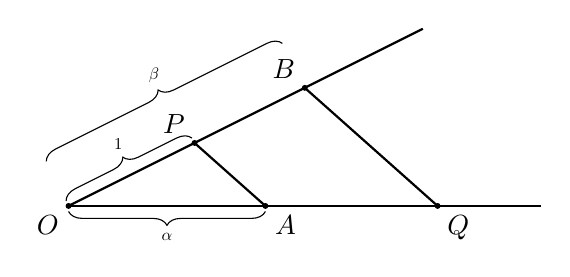
\begin{tikzpicture}
        \coordinate (O) at (0, 0);
        \node[below left] at (O) {\(O\)};

        \coordinate (A) at (2.5, 0);
        \node[below right] at (A) {\(A\)};

        \coordinate (B) at (3, 1.5);
        \node[above left] at (B) {\(B\)};

        \coordinate (P) at (1.6, 0.8);
        \node[above left] at (P) {\(P\)};

        \coordinate (Q) at (4.687, 0);
        \node[below right] at (Q) {\(Q\)};

        \filldraw[color=black] (O) circle (0.03);
        \filldraw[color=black] (A) circle (0.03);
        \filldraw[color=black] (B) circle (0.03);
        \filldraw[color=black] (P) circle (0.03);
        \filldraw[color=black] (Q) circle (0.03);

        \draw[thick] (O) -- (6, 0);
        \draw[thick] (O) -- (4.5, 2.25);
        \draw[thick] (P) -- (A);
        \draw[thick] (B) -- (Q);

        \draw[decorate,decoration={brace,raise=2pt,amplitude=5pt}] (O) -- (P)
            node[scale=0.6, midway, above=18pt, left=2pt] {\(1\)};
        \draw[decorate,decoration={brace,raise=18pt,amplitude=5pt}] (O) -- (B)
            node[scale=0.6, midway, above=43pt, left=13pt] {\(\beta\)};
        \draw[decorate,decoration={brace,mirror,raise=2pt,amplitude=5pt}] (O) -- (A)
            node[scale=0.6, midway, below=13pt] {\(\alpha\)};
    \end{tikzpicture}
    \qquad
    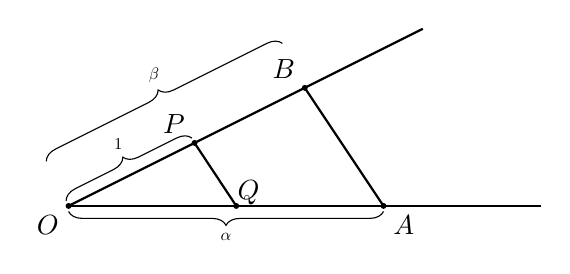
\begin{tikzpicture}
        \coordinate (O) at (0, 0);
        \node[below left] at (O) {\(O\)};

        \coordinate (A) at (4, 0);
        \node[below right] at (A) {\(A\)};

        \coordinate (B) at (3, 1.5);
        \node[above left] at (B) {\(B\)};

        \coordinate (P) at (1.6, 0.8);
        \node[above left] at (P) {\(P\)};

        \coordinate (Q) at (2.13, 0);
        \node[above right=-3pt] at (Q) {\(Q\)};

        \filldraw[color=black] (O) circle (0.03);
        \filldraw[color=black] (A) circle (0.03);
        \filldraw[color=black] (B) circle (0.03);
        \filldraw[color=black] (P) circle (0.03);
        \filldraw[color=black] (Q) circle (0.03);

        \draw[thick] (O) -- (6, 0);
        \draw[thick] (O) -- (4.5, 2.25);
        \draw[thick] (P) -- (Q);
        \draw[thick] (B) -- (A);

        \draw[decorate,decoration={brace,raise=2pt,amplitude=5pt}] (O) -- (P)
            node[scale=0.6, midway, above=18pt, left=2pt] {\(1\)};
        \draw[decorate,decoration={brace,raise=18pt,amplitude=5pt}] (O) -- (B)
            node[scale=0.6, midway, above=43pt, left=13pt] {\(\beta\)};
        \draw[decorate,decoration={brace,mirror,raise=2pt,amplitude=5pt}] (O) -- (A)
            node[scale=0.6, midway, below=13pt] {\(\alpha\)};
    \end{tikzpicture}
\end{center}

\rmk Since \(\Q\) is the smallest field containing \(\Z\), constructible real numbers contain \(\Q\). So constructible real numbers is an extension field of \(\Q\).

\pagebreak

Now, how about irrational numbers? We can construct \(\sqrt{2}\) by constructing a isosceles triangle and taking the hypotenuse. What else?

Let \(F\) be the set of constructible real numbers.

\thm. Any \(\alpha \in F\) can be represented using combinations of \(+\), \(-\), \(\times\), \(\div\) and \(\sqrt{\vphantom{l}}\).

\pf Idea. We have a straightedge and a compass, so we can use the equation of lines and circles. So we can \textit{only} get a combination of the above operations. Thus, if we can construct radicals, the theorem is trivial.

\begin{center}

    \usetikzlibrary {decorations.pathmorphing, decorations.pathreplacing, decorations.shapes}
    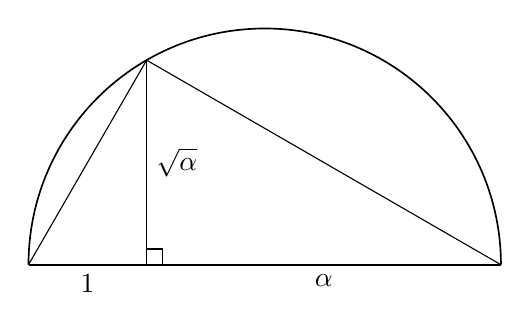
\begin{tikzpicture}
        \coordinate (A) at (-3, 0);
        \coordinate (B) at (3, 0);
        \coordinate (P) at (-1.5, 2.598);
        \coordinate (H) at (-1.5, 0);
        \draw[semithick] (A) arc(180:0:3) (B);
        \draw[semithick] (A) -- (B);
        \draw (P) -- (H) node[midway, right] {\(\sqrt{\alpha}\)};
        \draw (A) -- (P);
        \draw (B) -- (P);
        \draw (A) -- (H) node[midway, below] {\(1\)};
        \draw (B) -- (H) node[midway, below] {\(\alpha\)};
        \draw (H) rectangle (-1.3, 0.2);
    \end{tikzpicture}
\end{center}

\vspace*{-10pt}

\qed

Since we can use radicals, the degree of extension would be at most \(2\).

\cor. Let \(r\) be an irrational constructible number. Then there exists \(r_1, r_2, \dots, r_m = r \in \R\) such that
\[
    [\Q(r_1, \dots, r_l) : \Q(r_1, \dots, r_{l+1})] = 2
\]
for \(l = 1, 2, \dots, m - 1\). In particular, \([\Q(r) : \Q] = 2^n\) for some \(n \in \Z_{\geq 0}\).

\pf Each \(r_i\) occurs when we use radicals, so the existence of \(r_i\) is immediate, and radicals extend the field with degree \(2\), so the result follows. \qed

\section*{The Impossibility of Certain Constructions}

\thm. Doubling a cube is impossible. i.e, \(\sqrt[3]{2}\) is not constructible.

\pf Suppose that \(\sqrt[3]{2} \in F\). But \([\Q(\sqrt[3]{2}) : \Q] = 3\), which is not a power of \(2\). \qed

\thm. Squaring a circle is impossible. i.e, \(\sqrt{\pi}\) is not constructible.

\pf \(\pi\) is transcendental over \(\Q\), and so is \(\sqrt{\pi}\). \qed

\thm. Trisecting an arbitrary angle is impossible.

\pf Suppose we have an angle of \(60^\circ\). If constructing \(20^\circ\) is possible, then we can construct \(\cos 20^\circ\). Now we show that \(\cos 20^\circ\) is not constructible. From the identity \(\cos 3\theta = 4\cos^3 \theta - 3\cos\theta\), set \(\theta = 20^\circ\), and let \(\alpha = \cos \theta\). Then we have \(8\alpha^3 - 6\alpha - 1 = 0\), which is irreducible. Since \(\alpha\) is a zero, \([\Q(\alpha) : \Q] = 3\), which is a contradiction. \qed

\rmk Regular \(n\)-gon (\(n \geq 3\)) is constructible \(\iff\) the angle \(\frac{2\pi}{n}\) is constructible \(\iff\) \(\cos \frac{2\pi}{n}\) is constructible.

\pagebreak

\topic{Finite Fields}

Our goal is to determine the structure of all \textit{finite fields}, fields with finite order.

\thm. Let \(F\) be a finite field with \(\abs{F} = q\). If \(E\) is a finite extension of \(F\) with \([E : F] = n\), then \(\abs{E} = q^n\).

\pf \(E\) is an \(n\)-dimensional \(F\)-vector space. Trivial. \qed

\cor. Let \(E\) be a finite field with \(\ch E = p\). Then \(\abs{E} = p^n\) for some \(n \in \N\).\footnote{Note that \(p\) has to be prime.}

\pf Let \(1\) be the multiplicative identity of \(E\). Then \(\{1, 2 \cdot 1, \dots, p \cdot 1\} \simeq \Z_p \leq E\). Therefore \(E\) is a finite extension of a finite field \(\Z_p\), so we have \(\abs{E} = p^n\) for some \(n \in \N\). \qed

\thm. Let \(E \subset \bar{\Z_p}\) be a field with \(\ch E = p\) and \(\abs{E} = p^n\). Then
\begin{center}
    \(E \simeq \left\{ \text{zeros of } x^{p^n} - x \in \Z_p[x] \text{ in } \bar{\Z_p} \right\}\).
\end{center}

\pf Since \(E\) is a field, \(E\cross\) is a group and \(\abs{E\cross} = p^n - 1\). Then for \(a \in E\cross\), \(a^{\abs{E\cross}} = 1\). Thus \(a^{p^n - 1} - 1 = 0\), and \(a^{p^n} - a = 0\). Thus every element in \(E\) is a zero of \(x^{p^n} - x\). Since this polynomial can have at most \(p^n\) zeros, we are done. \qed

The zeros of the polynomial \(x^{p^n} - x \in \Z_p[x]\) describes \(E\).

\defn. \note{Root of Unity}
\begin{enumerate}
    \item \(\zeta\) is a \textbf{\(n\)-th root of unity} if \(\zeta^n = 1\).
    \item \(\zeta\) is a \textbf{primitive \(n\)-th root of unity} if \(\zeta^n = 1\) and \(\zeta^i \neq 1\) for \(1 \leq i < n\).
\end{enumerate}

Non-zero elements of a finite field of order \(p^n\) are all \((p^n - 1)\)-th roots of unity.

\cor. If \(F\) is a finite field and \(E\) is a finite extension of \(F\), then \(E\) is a simple extension.

\pf \(E\cross\) is a cyclic group, so suppose that \(\alpha \in E\cross\) is a generator. Then \(E = F(\alpha)\) by definition of simple extensions. \qed

Suppose \(\Z_p \leq E = \Z_p(\alpha) \leq K = E(\beta)\), where \(\alpha\) is algebraic over \(\Z_p\) and \(\beta\) is algebraic over \(E\). Then these are finite extensions, so \(K\) is a simple extension of \(F\). i.e, \(K = F(\gamma)\) for some \(\gamma\). The extension depends on which element you choose.

\pagebreak

\section*{Fields of Order \(p^n\) : \(\GF(p^n)\)}

We saw that if a finite field of order \(p^n\) is given, it is isomorphic to the zeros of \(x^{p^n} - x \in \Z_p[x]\). Now we want to see if a field of order \(p^n\) exists for any given \(p\) and \(n\).

We have two candidates. If there exists an irreducible polynomial \(f(x)\) of order \(n\) over \(\Z_p\), we know that \(\Z_p[x] \quotient \span{f(x)}\) is a finite field of order \(p^n\). Or we can try to show if the zeros of \(x^{p^n} - x\) form a field.

\lemma{1} \(x^{p^n} -x \in \Z_p[x]\) has \(p^n\) distinct zeros in \(\bar{\Z_p}\).

\pf Since the polynomial has degree \(p^n\) and \(0\) is a zero, we show that \(x^{p^n - 1} - 1\) has \(p^n - 1\) distinct zeros. Suppose that \(\alpha \in \bar{\Z_p}\) is a zero of \(x^{p^n - 1} - 1\). Then
\[\tag{\mast}
    \frac{x^{p^n - 1} - 1}{x - \alpha} = x^{p^n - 2} + \alpha x^{p^n-3} + \cdots + \alpha^{p^n - 2}.
\]
Set \(x = \alpha\), then (\mast) is equal to \((p^n - 1)\alpha^{p^n - 2} = -\alpha\inv \neq 0\), thus \(\alpha\) cannot be a multiple root. \qed

\lemma{2} If \(\alpha, \beta\) are zeros of \(x^{p^n} - x\), then \(\alpha \pm \beta\), \(\alpha\beta\), \(\alpha/\beta\) are also zeros of \(x^{p^n} - x\).

\pf Trivial. \qed

\thm. Let \(p\) be prime, and \(n \in \N\). Then there exists a field of order \(p^n\).

Thus, given a finite field \(F\), we can extend \(F\) with given dimension. Then the extension field \(E\) is a finite extension, thus \(E\) is a simple extension.

\cor. Let \(F\) be a finite field. For \(n \in \N\), there exists a irreducible polynomial \(p(x) \in F[x]\) of degree \(n\).

\pf Let \(\ch F = p\), then \(\abs{F} = p^r\) for some \(r \in \N\). Since elements of \(F\) are zeros of \(x^{p^r} - x\), we have \(\alpha^{p^{rn}} = \alpha\) for \(\alpha \in F\). Consider a finite field \(K\) of order \(p^{rn}\). Then \(\alpha \in K\), so \(F \leq K\). \(K\) is a finite extension of \(F\), so \(K\) must be a simple extension of degree \(n\). There is an element \(\beta \in K\) such that \(K = F(\beta)\), so \(\irr(\beta, F)\) is the polynomial we're looking for. \qed

Our next question is the uniqueness!

\thm. Let \(E, E'\) be fields of order \(p^n\). Then \(E \simeq E'\).

\pf \(E \simeq \Z_p[x] \quotient \span{p(x)}\) where \(p(x) \in \Z_p[x]\) is irreducible with degree \(n\). For any \(\alpha \in E\), \(\alpha^{p^n} - \alpha = 0\), so \(p(x) \mid (x^{p^n} - x)\). In addition, \(E'\) also consists of zeros of \(x^{p^n} - x\), so \(E'\) has a zero of \(p(x)\). Since \(E'\) has order \(p^n\), then we have \(E' \simeq \Z_p[x] \quotient \span{p(x)} \simeq E\).

Conclusion. For a prime \(p\) and \(n \in \N\), there exists a unique field of order \(p^n\), up to isomorphism. Furthermore, this field is a simple extension field of order \(p^m\) (\(m < n\)), and contains zeros of \(x^{p^n} - x \in \Z_p[x]\).

\pagebreak

\setcounter{chapter}{6}

\chapter{Advanced Group Theory}

We briefly review advanced group theory from last semester.

\setcounter{topic}{33}
\topic{Isomorphism Theorems}

\thm. \note{First Isomorphism Theorem} Let \(\varphi : G \ra G'\) be a group homomorphism. Then \(\bar{\varphi} : G \quotient \ker \varphi \ra \im \varphi\) defined as
\[
    \bar{\varphi}(\bar{x}) = \varphi(x), \quad (x \in G)
\]
is an isomorphism, and \(G \quotient \ker \varphi \simeq \im \varphi\).
\[
    \begin{tikzcd}
        G \arrow{rr}{\varphi} \arrow[swap]{dr}{\pi} & \arrow[d, phantom, "\circlearrowright"]& \im \varphi \\
        & G \quotient \ker\varphi \arrow[dashed,swap]{ur}{\bar{\varphi}} &
    \end{tikzcd}
\]

\thm. \note{Second Isomorphism Theorem} If \(H \leq G\) and \(N \nsub G\),
\[
    \frac{HN}{N} \simeq \frac{H}{H\cap N}.
\]
\begin{center}
    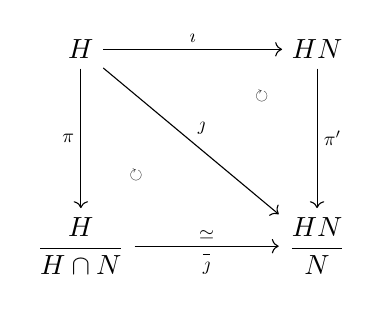
\begin{tikzpicture}
        \node (H) at (0, 0) {\(H\)};
        \node (HN) at (3, 0) {\(HN\)};
        \node (HoverHcapN) at (0, -2.5) {\(\dfrac{H}{H \cap N}\)};
        \node (HNoverN) at (3, -2.5) {\(\dfrac{HN}{N}\)};

        \draw[->] (H) -- (HN) node[midway,above,scale=0.7] {\(\imath\)};
        \draw[->] (HN) -- (HNoverN) node[midway,right,scale=0.7] {\(\pi'\)};
        \draw[->] (H) -- (HoverHcapN) node[midway,left,scale=0.7] {\(\pi\)};
        \draw[->] (HoverHcapN) -- (HNoverN) node[midway,below,scale=0.7] {\(\bar{\jmath}\)} node[midway,above,scale=0.7] {\(\simeq\)};
        \draw[->] (H) -- (HNoverN) node[midway,above right,scale=0.7] {\(\jmath\)};

        \node[scale=0.6] at (0.7, -1.6) {\(\circlearrowright\)};
        \node[scale=0.6] at (2.3, -0.6) {\(\circlearrowright\)};
    \end{tikzpicture}
\end{center}

\thm. \note{Third Isomorphism Theorem} If \(H, K \nsub G\) and \(K \leq H\),\footnote{This implies that \(K \nsub H\).} then
\[
    G \quotient H \simeq \frac{G \quotient K}{H \quotient K}.
\]

\topic{Series of Groups}

\defn. Given a finite sequence of subgroups
\[
    \{e\} = H_0 < H_1 < \cdots < H_k = G,
\]
\begin{enumerate}
    \item \note{Subnormal Series} If \(H_i \pnsub H_{i+1}\) for \(i = 0, \dots, k - 1\), it is called a \textbf{subnormal series}.
    \item \note{Normal Series} If \(H_i \pnsub G\) for \(i = 0, \dots, k - 1\), it is called a \textbf{normal series}.
\end{enumerate}

\rmk Since \(H_i \pnsub G \implies H_i \pnsub H_{i+1}\), a normal series is a subnormal series.

We want to decompose a group \(G\) into normal subgroups. We focus on the quotient groups that appear in the series.

\defn. \note{Refinement} For two subnormal (normal) series \(\seq{H_i}\) and \(\seq{K_j}\) of \(G\), \(\seq{K_j}\) is a \textbf{refinement} of \(\seq{H_i}\) if \(\seq{H_i} \subset \seq{K_j}\).

\defn. Subnormal (normal) series \(\seq{H_i}_{i \in I}\), \(\seq{K_j}_{j \in J}\) of \(G\) are \textbf{isomorphic} if there exists a bijection between
\[
    \{H_{i+1} / H_i\} \longleftrightarrow \{K_{j+1} / K_j\}
\]
such that the corresponding quotient groups are isomorphic.

\thm. \note{Schrier} Any two subnormal (normal) series of \(G\) have isomorphic refinements.

\defn. Let \(\seq{H_i}\) be a subnormal (normal) series of \(G\). If \(H_{i+1} \quotient H_i\) is simple for any \(i\), \(\seq{H_i}\) is called a \textbf{composition (principal) series}.

\thm. \note{Jordan-Hölder} Any two composition series of a group \(G\) are isomorphic.

\defn. \note{Solvable Group} A group \(G\) is \textbf{solvable} if there exists a composition series \(\seq{H_i}\) such that all quotient groups are abelian.

\pagebreak

\topic{Sylow Theorems}

Sylow theorems are very important in finite group theory. When we first learned groups, we tried to classify groups of finite order. For example, if \(\abs{G} = 2\), then \(G \simeq \Z_2\), if \(\abs{G} = 4\), then \(G \simeq \Z_4\) or \(\Z_2 \times \Z_2\). But for groups with order above \(6\), it is very hard to classify them. Since the ultimate goal of group theory is to classify the groups, Sylow theorems were devised as a tool for classifying groups. Recall Lagrange's theorem. For a finite group \(G\), if \(H \leq G\), then \(\abs{H} \mid \abs{G}\). It is often important to analyze the structures of subgroups. Sylow theorems give us the converse for some cases.

In the context of this class, Sylow theorems are important as an application of group actions, and we also use the theorems later for Galois theory.

We start with some review.

\defn. \note{Group Action} Let \(G\) be a group and \(X\) be a \(G\)-set. A \textbf{group action} of \(G\) on \(X\) is a map \(G \times X \ra X\) such that
\begin{enumerate}
    \item If \(e\) is the identity of \(G\), \(ex = x\) for all \(x \in X\).
    \item \((g_1g_2)x = g_1(g_2 x)\) for all \(g_1, g_2 \in G\) and \(x \in X\).
\end{enumerate}

\rmk Given a finite \(G\)-set \(X\), we can partition \(X\) in to orbits of \(X\) using the equivalence class defined as
\begin{center}
    \(x_1 \sim x_2\) if and only if \(x_1 = g x_2\) for some \(g \in G\).
\end{center}
Then the equivalence classes were called \textbf{orbits}, written as \(Gx\).

\prop. \note{Class Equation} Let \(x_i\) be representatives from each orbit. Then \(\abs{X} = \sum_{i} \abs{Gx_i}\). Consider orbits of size \(1\). Then we see that if \(\abs{Gx} = 1\) for some \(x\), then \(gx = x\) for all \(g \in G\). Let \(X_G = \{x \in X : gx = x, \forall g \in G\}\). Then we have
\[ \tag{\mast}
    \abs{X} = \abs{X_G} + \sum \abs{G x_i}
\]
where the summation is over \(x_i\) with \(\abs{G x_i} \geq 2\).

\prop. \(\abs{Gx} = \ind{G}{G_x}\) for all \(x \in X\), so \(\abs{Gx} \mid \abs{G}\).

\pf Section 16. \qed

\bigskip

On to the Sylow theorems. Let \(G\) be a (finite) group.

\thm. Let \(\abs{G} = p^n\) and let \(X\) be a finite \(G\)-set. Then \(\abs{X} \equiv \abs{X_G} \pmod p\).

\pf By (\mast), we show that \(\sum \abs{G x_i}\) is divisible by \(p\). Also by the above proposition, \(\abs{Gx} \mid \abs{G}\) but since \(G\) has prime order, \(\abs{Gx}\) is either \(1\) or a power of \(p\). But the summation is over \(x_i\) that are in orbits of order greater than 1, so \(\abs{Gx}\) is divisible by \(p\). \qed

\pagebreak

\thm. \note{Cauchy} If \(p \mid \abs{G}\) for prime \(p\), there exists an element of order \(p\) in \(G\).

\pf Let
\[
    X = \{(a_1, \dots, a_p) : a_1, \dots, a_p \in G, a_1a_2\cdots a_p = e\}.
\]
Then \(\abs{X} = \abs{G}^{p-1}\), since \(a_p\) is automatically fixed after choosing \(a_1, \dots, a_{p-1}\). Thus \(p \mid \abs{X}\).

Consider \(\sigma = (1, 2, \dots, p) \in S_p\) and \(\span{\sigma} \leq S_p\). Note that \(\abs{\span{\sigma}} = p\). Define \(\span{\sigma}\)-action on \(X\) by
\[
    \sigma(a_1, \dots, a_p) = (a_2, \dots, a_p, a_1).
\]
Then we can check that \((a_2, \dots, a_p, a_1) \in X\), and that this is indeed a group action.

Consider \(X_{\span{\sigma}} = \{(a, a, \dots, a) : a \in G, a^p = e\}\). If \((a, \dots, a) \in X_{\span{\sigma}}\), then \(\abs{a}\) must be either \(1\) or \(p\). Now it suffices to show that \(X_{\span{\sigma}}\) has an element that is not \((e, \dots, e)\).

By the above theorem, \(\abs{X_{\span{\sigma}}} \equiv 0 \pmod p\). But \((e, \dots, e) \in X_{\span{\sigma}} \neq \varnothing\), so there is a nontrivial element \(a \in G\) such that \(a^p = e\). Thus \(\abs{a} = p\) in \(G\).\footnote{Whenever we solve a problem using group actions, it is important to set the sets \(X\) and \(G\) properly...} \qed

\defn. \note{\(p\)-group} Let \(p\) be prime.
\begin{enumerate}
    \item \(G\) is called a \textbf{\(p\)-group} if the order of every element of \(G\) is a power of \(p\).
    \item A subgroup \(H \leq G\) is called a \textbf{\(p\)-subgroup} if \(H\) is a \(p\)-group.
\end{enumerate}

\cor. \(G\) is a \(p\)-group if and only if \(\abs{G} = p^n\) for some \(n \in \Z_{\geq 0}\).

\pf \note{\mimpd} For \(a \in G\), \(\abs{a} \mid \abs{G}\). Hence \(\abs{a} = p^m\) for some \(m \in \Z_{\geq 0}\), and \(G\) is a \(p\)-group.

\note{\mimp} Suppose that \(\abs{G} = p^n q N\) for some prime \(q \neq p\). By Cauchy's theorem, \(G\) has an element of order \(q\). Thus \(G\) cannot be a \(p\)-group. \qed

\section*{Sylow Theorems}

\defn. \note{Normalizer} For subgroup \(H\) of \(G\), the \textbf{normalizer} of \(H\) is defined as
\[
    N[H] = \{a \in G : aHa\inv = H\}.
\]

By definition, \(H \nsub N[H]\). Also, it is the largest subgroup of \(G\) that has \(H\) as a normal subgroup.

\lemma. Let \(G\) be a finite group and let \(H\) be a \(p\)-subgroup of \(G\). Then
\[
    \ind{N[H]}{H} \equiv \ind{G}{H} \pmod p.
\]

\pf Let \(\mc{L}\) be the left cosets of \(H\) in \(G\). Then by definition, \(\abs{\mc{L}} = \ind{G}{H}\). Define \(H\)-action on \(\mc{L}\) by \(h\bar{x} = \bar{hx}\). Then \(\mc{L}_H = \left\{\bar{x} \in \mc{L} : \bar{hx} = \bar{x}, \forall h \in H\right\}\).

If \(\bar{hx} = \bar{x}\) for all \(h \in H\), \(x\inv h x \in H\) for all \(h \in H\). Thus \(x \in N[H]\) and \(\abs{\mc{L}_H} = \ind{N[H]}{H}\). \(H\) is a \(p\)-subgroup, so it has order of prime power by the above corollary. We have the desired result by \(\abs{\mc{L}} \equiv \abs{\mc{L}_H} \pmod p\).\qed

\bigskip

\thm. \note{First} Let \(G\) be a finite group of order \(p^n \cdot m\) with \(\gcd(p, m) = 1\) and \(n \geq 1\).
\begin{enumerate}
    \item For \(i \in \{1, \dots, n\}\), there exists a subgroup of order \(p^i\).
    \item For any subgroup \(H\) of order \(p^i\) (\(1 \leq i \leq n - 1\)), there exists a subgroup \(K\) of order \(p^{i+1}\) such that \(H \nsub K\).
\end{enumerate}

The existence of the a \(p\)-subgroup of order \(p^n\) is guarenteed by the theorem.

\pf We use induction. The case \(i = 1\) is true by Cauchy's theorem. Next, we construct a subgroup of order \(p^{i+1}\) from a subgroup of order \(p^i\).

Consider \(N[H] \quotient H\). Then by the above lemma, \(p \mid \abs{N[H] \quotient H}\). By Cauchy's theorem again, choose \(a \in N[H] \quotient H\) such that \(\abs{a} = p\).

Let \(\pi\) be the canonical projection. Then \(K = \pi\inv(\span{a})\) has order \(p^{i+1}\), and \(K \leq N[H] \leq G\). Moreover, since \(H < K \leq N[H]\) and \(H \nsub N[H]\), we have \(H \nsub K\). \qed

\bigskip

\defn. \note{Sylow \(p\)-subgroup} A maximal \(p\)-subgroup of \(G\) is called a \textbf{Sylow \(p\)-subgroup}.\footnote{Sylow \(p\)-subgroups need not be unique.}

By the first Sylow Theorem, if \(\abs{G} = p^n \cdot m\) (\(\gcd(p, m) = 1\)), then a Sylow \(p\)-subgroup of \(G\) has order \(p^n\). If \(G\) is a finite group, it is easy to check if a subgroup is a Sylow \(p\)-subgroup, by counting the number of elements.

\thm. \note{Second} Let \(P_1\), \(P_2\) be Sylow \(p\)-subgroups. Then \(P_1\) and \(P_2\) are conjugate. (i.e. there is an element \(x \in G\) such that \(x\inv P_1 x = P_2\))

\pf Let \(\mc{L}\) be the set of left cosets of \(P_1\) in \(G\). \(P_2\) acts on \(\mc{L}\) by \(y \bar{x} = \bar{yx}\) for \(x \in G\), \(y \in P_2\). (\(\mc{L}\) is a \(P_2\)-set) (Check that this is a group action) Then \(\abs{\mc{L}} \equiv \abs{\mc{L}_{P_2}} \pmod p\).

Since \(P_1\) is a Sylow \(p\)-subgroup, \(p \nmid \ind{G}{P_1} = \abs{\mc{L}}\). So \(\abs{\mc{L}_{P_2}} \neq 0\). Choose some \(\bar{x} \in \mc{L}_{P_2}\), then for any \(y \in P_2\), \(y\bar{x} = \bar{x}\). Therefore \(x\inv P_2 x \leq P_1\), but \(\abs{P_1} = \abs{P_2}\), so \(x\inv P_2 x = P_1\). \qed

\bigskip

\thm. \note{Third} Let \(G\) be a finite group with \(p \mid \abs{G}\). Let \(s\) be the number of Sylow \(p\)-sub\-groups. Then \(s \equiv 1 \pmod p\) and \(s \mid \abs{G}\).

\pf Let \(P\) be a Sylow \(p\)-subgroup of \(G\), and let \(\mc{S}\) be the set of all Sylow \(p\)-subgroups. We define a group action on \(\mc{S}\), as \(xT = xTx\inv\) for \(x \in P\) and \(T \in \mc{S}\). Then \(\abs{\mc{S}} \equiv \abs{\mc{S}_P} \pmod p\). Now observe that \(T \in \mc{S}_P\) if and only if \(xTx\inv = T\) for all \(x \in P\). This implies \(P \subset N[T]\).

Note that \(T\) and \(P\) are Sylow \(p\)-subgroups of \(G\). Also, \(P,\, T \leq N[T] \leq G\). Thus \(P\), \(T\) are Sylow \(p\)-subgroups of \(N[T]\). By the second Sylow theorem, \(P\) and \(T\) are conjugate in \(N[T]\). But since \(T \nsub N[T]\), any conjugate of \(T\) in \(N[T]\) should be equal to itself, so \(P = T\). \(\mc{S}_P = \{P\}\), so \(\abs{\mc{S}} \equiv \mc{\mc{S}_P} \equiv 1 \pmod p\).

For the last statement, consider \(G\)-action on \(\mc{S}\) by conjugation. By second Sylow theorem, all Sylow \(p\)-subgroups are conjugate, so \(\mc{S}\) consists of a single orbit. Then \(\abs{\mc{S}}\) is equal to the number of elements in \(GP\) (orbit), which equals \(\ind{G}{G_P}\). Thus \(\abs{\mc{S}} \mid \abs{G}\). \qed

\ex. Consider the symmetric group \(S_3 = \{id, (1, 2), (1, 3), (2, 3), (1, 2, 3), (1, 3, 2)\}\).
\begin{itemize}
    \item Sylow \(2\)-subgroups are subgroups of order \(2\). \(\{id, (1, 2)\}\), \(\{id, (1, 3)\}\), \(\{id, (2, 3)\}\). There are \(3\) of them, and \(3 \equiv 1 \pmod 2\) and \(3 \mid \abs{S_3}\). The third Sylow theorem works.
    \item Let \(P_1 = \{id, (1, 2)\}\), then \((1, 3) P_1 (1, 3) = \{id, (2, 3)\}\). Also \((2, 3)P_1(2, 3) = \{id, (1, 3)\}\). Sylow \(2\)-subgroups are conjugate. The second Sylow theorem works.
\end{itemize}

Sylow theorems helps us classify finite simple groups.

\ex. No group of order \(15\) is simple.

\pf Let \(\abs{G} = 15\). Then there exists a Sylow \(5\)-subgroup \(P\) of order \(5\) by first Sylow theorem. If there exists another Sylow \(5\)-subgroup \(P'\), then \(P\) and \(P'\) are conjugate by second Sylow theorem. Thus, if \(G\) has a unique Sylow \(5\)-subgroup, then it is a normal subgroup.\footnote{This is because for each \(g \in G\), the inner automorphism \(i_g\) of \(G\) maps \(P\) onto a subgroup \(gPg\inv\), again of order \(5\). We use this fact very often when determining that groups with some order cannot be simple.} Now we check how many Sylow \(5\)-subgroups there are. Let \(k\) be the number of Sylow \(5\)-subgroups of \(G\), then \(k \mid 15\) and \(k \equiv 1 \pmod 5\). Then \(k = 1\), we are done. \qed

\section*{Sylow Theorems (Summary)}

\thm. \note{First} Let \(G\) be a finite group of order \(p^n \cdot m\) with \(\gcd(p, m) = 1\) and \(n \geq 1\).
\begin{enumerate}
    \item For \(i \in \{1, \dots, n\}\), there exists a subgroup of order \(p^i\).
    \item For any subgroup \(H\) of order \(p^i\) (\(1 \leq i \leq n - 1\)), there exists a subgroup \(K\) of order \(p^{i+1}\) such that \(H \nsub K\).
\end{enumerate}

\thm. \note{Second} Let \(P_1\), \(P_2\) be Sylow \(p\)-subgroups. Then \(P_1\) and \(P_2\) are conjugate.

\thm. \note{Third} Let \(G\) be a finite group with \(p \mid \abs{G}\). Let \(s\) be the number of Sylow \(p\)-subgroups. Then \(s \equiv 1 \pmod p\) and \(s \mid \abs{G}\).

\pagebreak

\topic{Applications of the Sylow Theory}

\thm. Every finite \(p\)-group is solvable.

\pf Let \(G\) be a group of order \(p^n\). By first Sylow theorem, \(G\) has subgroups \(H_i\) of order \(p^i\) that is normal in subgroups \(H_{i+1}\) of order \(p^{i+1}\) \((1 \leq i < n)\). So there is a subnormal series
\[
    \{e\} < H_1 < H_2 < \cdots < H_n = G
\]
such that \(\abs{H_{i+1} \quotient H_i} = p\). Then \(H_{i+1} \quotient H_i \simeq \Z_p\), which is abelian and simple. Thus the subnormal series is a composition series. \qed

\thm. \(Z(G)\) is nontrivial for finite \(p\)-group \(G\).

\pf Let \(G\) act on itself by conjugation. Then \(X_G = Z(G)\), so \(\abs{G} = \abs{Z(G)} + \sum \abs{Gx_i}\), where the summation is over orbits of length greater than 1. Since \(\abs{Gx_i} \mid \abs{G}\), (\(\abs{Gx_i}\) is a power of prime) we have \(p \mid \abs{Z(G)}\). But \(e \in Z(G)\), so \(\abs{Z(G)} \geq p\). \qed

We can break down large groups into smaller groups.

\lemma. Let \(H, K \nsub G\). If \(H \cap K = \{e\}\) and \(H \vee K = G\),\footnote{\(G = \span{H, K}\).} then \(G \simeq H \times K\).

\pf We show that \(\varphi : H \times K \ra G\) defined as \((h, k) \mapsto hk\) is an isomorphism.
\begin{enumerate}
    \item (Homomorphism) Note that \(hkh\inv k\inv \in K \cap H = \{e\}\), so \(h\) and \(k\) commute.
    \[
        \varphi(h, k) \varphi(h', k') = hkh'k' = hh'kk' = \varphi\paren{(h, k)(h', k')}.
    \]
    \item (Injective) Suppose that \(\varphi(h, k) = hk = e\). Then \(h = k\inv \in H\cap K\), so \(h = k = e\).
    \item (Surjective) \(H \vee K = HK = G\) by hypothesis.\footnote{Check \sref{Lemma 34.4}.} Trivial. \qed
\end{enumerate}

\thm. If \(\abs{G} = p^2\), then \(G\) is abelian.

\pf If there is an element of order \(p^2\), then \(G \simeq \Z_{p^2}\), so we are done. Otherwise, take \(a \in G \bs \{e\}\). Then \(\abs{a}\) must be \(p\). Now take \(b \in G \bs \span{a}\). Then \(\abs{b}\) must also be \(p\). We want to use the above lemma.
\begin{enumerate}
    \item \(\span{a}, \span{b} \nsub G\) by the first Sylow theorem.
    \item If \(e \neq c \in \span{a} \cap \span{b}\), then \(\span{c} \leq G\), \(\abs{c}\) must be \(p\) by Lagrange's theorem. Then \(c\) would generate both \(\span{a}, \span{b}\).
    \item Suppose \(a^mb^n = a^{m'}b^{n'}\), then \(a^{m-m'} = b^{n'-n}\) must be \(e\). Then \(m = m'\), \(n = n'\) in \(\Z_p\). Since \(\{a^mb^n : m, n \in \Z\} \subset \span{a} \vee \span{b}\), so \(p^2 \leq \abs{\span{a} \vee \span{b}}\). But \(\span{a} \vee \span{b} = \span{a}\span{b} \nsub G\), so it must have order \(p^2\) and \(\span{a} \vee \span{b} = G\).
\end{enumerate}
Therefore, \(G \simeq \span{a} \times \span{b} \simeq \Z_p \times \Z_p\). \qed

\thm. Let \(\abs{G} = pq\) for distinct primes \(p, q\) with \(p < q\).
\begin{enumerate}
    \item \(G\) is not simple. (\(G\) has a normal subgroup of order \(q\))
    \item If \(q \not\equiv 1 \pmod p\), then \(G\) is abelian.
\end{enumerate}

\pf \note{1} By the third Sylow theorem, the number of Sylow \(q\)-subgroups must be either \(1, p, q, pq\), and the only possibility is \(1\). So \(G\) has a unique Sylow \(q\)-subgroup, and \(G\) is not simple.

\note{2} We show that \(G \simeq \Z_p \times \Z_q\). Let \(H\) be the unique Sylow \(q\)-subgroup of \(G\). Since \(q \not\equiv 1 \pmod p\), there can only be a unique Sylow \(p\)-subgroup \(K\). We use the above lemma again.
\begin{enumerate}
    \item \(H, K \nsub G\) since they are unique Sylow \(p\), \(q\)-subgroups.
    \item \(\abs{H \cap K} \mid p\) and \(q\), so \(H \cap K\) must have order \(1\), so \(H \cap K = \{e\}\).
    \item \(\abs{H \vee K}\) must be a multiple of \(p, q\) but should be a divisor of \(pq\), thus \(\abs{H \vee K} = pq\) and \(H \vee K = G\).
\end{enumerate}
Thus \(G \simeq H \times K \simeq \Z_p \times \Z_q\). \qed

We haven't seen many examples yet, but they will help us answer many classification questions. The last lemma is a technical lemma for applications.

\lemma. Let \(H, K\) be finite subgroups of \(G\).\footnote{Compare this with the second isomorphism theorem. We needed a subgroup to be \textit{normal}.} Then
\[
    \abs{HK} = \frac{\abs{H} \abs{K}}{\abs{H \cap K}}.
\]

\pf We show that \(\varphi : HK \times (H \cap K) \ra H \times K\) is a bijection.

\note{\(\geq\)} For \(hk \in HK\), choose \(x \in H \cap K\) and set \(h' = hx\), \(k' = x\inv k\). Then \(h'k' = hk\). Each element in \(HK \times (H \cap K)\) is mapped to a different element \((h', k') \in H \times K\).

\note{\(\leq\)} For each \((h, k) \in H \times K\), choose \(y \in H\cap K\) so that \(h'' = hy\inv\), \(k'' = yk\). Then \(h''k'' = hk\). Each element of \(H \times K\) is mapped to a different element \((hk, y) \in HK \times (H \cap K)\). \qed

\medskip

We will now see examples where Sylow theorems can be used.

\ex. Let \(\abs{G} = p^r\) (\(r \geq 2\)). (finite \(p\)-group) By the first Sylow theorem, there exists a normal subgroup of order \(p^{r-1}\). Thus \(G\) is not simple. \qed

\ex. Let \(\abs{G} = 15\). Since \(15 = 3 \times 5\), \(G\) is not simple and \(G \simeq \Z_{3\times 5}\) by the above theorem. \qed

\ex. Let \(\abs{G} = 20\). Note that \(20 = 2^2 \times 5\).
\begin{itemize}
    \item The number of Sylow \(2\)-subgroups can be either 1 or 5 by the third Sylow theorem.
    \item The number of Sylow \(5\)-subgroups should be 1 also by the third Sylow theorem.
\end{itemize}
Hence the Sylow \(5\)-subgroup of \(G\) is unique, so it is normal and \(G\) is not simple. \qed

We always check the number of Sylow \(p\)-subgroups first.

\ex. Let \(\abs{G} = 30\). Note that \(30 = 2 \times 3 \times 5\). By the third Sylow theorem,
\begin{itemize}
    \item The number of Sylow \(2\)-subgroups is either 1, 3, 5 or 15.
    \item The number of Sylow \(3\)-subgroups is either 1 or 10.
    \item The number of Sylow \(5\)-subgroups is either 1 or 6.
\end{itemize}
Our situation is not as simple as last time. We have to show that the number of Sylow \(p\)-subgroups is \(1\) for some \(p\).

So suppose that the number of Sylow \(3\)-subgroups is \(6\) and the number of Sylow \(5\)-subgroups is \(6\). Let \(P_1, \dots, P_{10}\) be distinct Sylow \(3\)-subgroups and \(Q_1, \dots, Q_6\) be distinct Sylow \(5\)-subgroup of \(G\).

We know that \(\abs{P_i} = 3\) and \(\abs{Q_i} = 5\). Our claim is that \(P_i \cap P_j = \{e\}\) for \(i \neq j\). This is because a group of order \(3\) is isomorphic to \(\Z_3\) and is generated by any element other than \(e\). Using a similar argument for \(Q_i\), we have
\[
    \abs{\bigcup_{i=1}^{10} P_i} = 1 + 2 \times 10 = 21, \quad \abs{\bigcup_{i=1}^6 Q_i} = 1 + 4 \times 6 = 25.
\]
Thus
\[
    \abs{\bigcup_{i=1}^{10} P_i \cup \bigcup_{i=1}^6 Q_i} = \overbrace{1}^{\text{identity}} + \overbrace{20}^{\text{order 3 elements}} + \overbrace{24}^{\text{order 5 elements}} = 45.
\]
But \(\abs{G} = 30\), contradiction. Thus either the number of Sylow \(3\)-subgroups or \(5\)-subgroups must be \(1\), therefore \(G\) is not simple. \qed

\ex. Let \(\abs{G} = 48\). Note that \(48 = 2^4 \times 3\). If there is a unique Sylow \(2\)-subgroup, we are done, so assume not. Let \(H, K\) be distinct Sylow \(2\)-subgroups. By the lemma above,
\[
    \abs{HK} = \frac{\abs{H} \abs{K}}{\abs{H \cap K}} = \frac{16 \times 16}{\abs{H \cap K}} \leq \abs{G} = 48.
\]
Thus \(\abs{H \cap K}\) should be at least \(6\), and should divide \(16\), since \(H \cap K\) is a subgroup of \(H\) and \(K\). Then the only possibility is \(\abs{H \cap K} = 8\). Then \(\ind{H}{H \cap K} = \ind{K}{H \cap K} = 2\), so \(H \cap K \nsub H, K\).

Now we consider \(N[H \cap K]\).\footnote{We actually want this group to be equal to \(G\)...}
\begin{itemize}
    \item By the above result, \(H, K \leq N[H \cap K]\). Thus \(16 \mid \abs{N[H \cap K]}\).
    \item \(N[H \cap K] > 16\), since it contains two distinct groups \(H\) and \(K\) of order \(16\).
    \item \(N[H \cap K] \leq G\), so \(\abs{N[H\cap K]} \mid 48\).
\end{itemize}

Overall, \(\abs{N[H\cap K]} = 48\) and \(N[H \cap K] = G\), so \(H \cap K \nsub G\) and \(G\) is not simple. \qed

\ex. Let \(\abs{G} = 3 \times 5 \times 17\). \(G\) is abelian and cyclic.

\pf We only have to show that \(G\) is abelian, because if \(G\) is abelian, \(G\) is cyclic by the fundamental theorem of finitely generated abelian groups. We will show that the commutator subgroup \(C(G)\) is trivial.

By the third Sylow theorem, \(G\) has a unique Sylow \(17\)-subgroup \(H\), and \(H \nsub G\). We consider \(G \quotient H\), which has \(15\) elements. In fact, \(G \quotient H \simeq \Z_{15}\) by the above example, thus it is abelian and cyclic. Recall that \(C(G) \leq N\) if and only if \(G \quotient N\) is abelian. So \(C(G) \leq H\), so \(C(G)\) must have order \(1\) or \(17\).

Again by the third Sylow theorem,
\begin{itemize}
    \item The number of Sylow \(3\)-subgroups is either \(1\) or \(85\).
    \item The number of Sylow \(5\)-subgroups is either \(1\) or \(51\).
\end{itemize}
Using a similar argument as above, we cannot have \(85\) distinct Sylow \(3\)-subgroups and \(51\) distinct Sylow \(5\)-subgroups at the same time. Check that \(1 + 2 \times 85 + 4 \times 51 = 375 > \abs{G}\). So either there is a unique Sylow \(3\)-subgroup, or a unique Sylow \(5\)-subgroup.
\begin{itemize}
    \item If \(G\) has a unique Sylow \(3\)-subgroup \(H_3\). Then it is normal, so \(G \quotient H_3 \simeq \Z_{85}\) and is abelian. Then \(C(G) \leq H_3\), so \(C(G)\) must have order \(1\) or \(3\).

    \item If \(G\) has a unique Sylow \(5\)-subgroup \(H_5\). Similarly, \(G \quotient H_5 \simeq \Z_{51}\), so \(C(G) \leq H_5\) and \(C(G)\) must have order \(1\) or \(5\).
\end{itemize}
Since \(C(G)\) must have order \(1\) or \(17\), we see that \(C(G)\) must be \(\{e\}\) for both cases. \qed

Sylow theorems will be used again when we study more field theory. We will not use them to classify finite groups, but the ideas and techniques in the proofs will be used again.

\pagebreak

\topic{Free Abelian Groups}

Free abelian groups are similar to vector spaces, and they are isomorphic to \(\Z^n\).

\thm. Let \(G\) be a nontrivial abelian group and let \(X \subset G\). The following are equivalent.

\begin{enumerate}
    \item Any \(a \in G\) can be uniquely expressed as \(a = n_1x_2 + n_2x_2 + \cdots + n_rx_r\), where \(x_i \in X\) are distinct and \(n_i \in \Z \bs \{0\}\).\footnote{Uniqueness is up to order, and 0 is excluded for uniqueness.}
    \item (i) \(\span{X} = G\), (ii) \(n_1x_1 + \cdots + n_rx_r = 0\) for distinct \(x_i \in X\) if and only if \(n_1 = \cdots = n_r = 0\).
\end{enumerate}

\pf Trivial. \qed

\rmk The condition in (2) seems somewhat similar to the condition of linearly independent vectors. Recall that in linear algebra, if \(\mf{B} = \{x_1, \dots, x_r\}\) is a basis of \(V\), then
\[
    V = x_1\R \oplus \cdots \oplus x_r \R \simeq \R \oplus \cdots \oplus \R \simeq \R^r,
\]
so \(\dim V\) is all we needed to classify vector spaces. Free abelian groups also satisfy this kind of property, they have a \textit{basis}.

\defn. \note{Free Abelian Group} If an abelian group \(G\) satisfies the conditions in the above theorem, \(G\) is a \textbf{free abelian group}, and the set \(X\) is called a \textbf{basis}.

\ex.
\begin{enumerate}
    \item \(\Z \times \Z \times \cdots \times \Z\) is a free abelian group. The basis is \(\{(1, 0, \dots, 0), \dots, (0, \dots, 0, 1)\}\). Note that the basis is not unique, as it was in vector spaces.
    \item \(\Z_n\) is not a free (abelian) group, since \(nx = 0\) for all \(x \in \Z_n\).
\end{enumerate}

\thm. Let \(G\) be a free abelian group with \(r\) basis elements. Then \(G \simeq \Z^r\).

\pf Let \(X = \{x_1, \dots, x_r\}\) be a basis of \(G\). Consider a group homomorphism \(\varphi : G \ra \Z^r\) as \(nx_i \mapsto (0, \dots, n, 0, \dots, 0)\). (\(n\) is in the \(i\)-th component) Then \(\varphi\) is an isomorphism. \qed

So now we know the complete structure of free abelian groups with finite basis. Bases are not unique but we can show that the number of elements in any bases are the same.

\thm. Let \(G\) be a free abelian group with finite basis. Then any basis of \(G\) have the same number of elements.

\pf By the above theorem, suppose that \(G \simeq \Z^r \simeq \Z^s\) with \(r\neq s\). Then \(G \quotient 2G \simeq \Z^r \quotient 2\Z^r \simeq \Z^s \quotient 2\Z^s\). But \(\Z^r \quotient 2\Z^r\) has order \(2^r\), while \(\Z^s \quotient 2\Z^s\) has order \(2^s\). But \(2^r \neq 2^s\), so cannot be isomorphic. \qed

These are very similar things we did in linear algebra. For vector space \(V\), the basis is not unique, but all bases have the same number of elements, and we called it the \textit{dimension} of a vector space. But in group theory, we give the name \textit{rank}. The above theorem shows that the rank is well-defined.

\defn. \note{Rank} Let \(G\) be a free abelian group. Then the \textbf{rank} of \(G\) is the number of elements in a basis of \(G\).

\subsection*{Proof of the Fundamental Theorem of Finitely Generated Abelian Groups}

\recall Let \(G\) be a finitely generated abelian group. Then
\[ \tag{\mast}
    G \simeq \Z_{p_1^{r_1}} \times \Z_{p_2^{r_2}} \times \cdots \times \Z_{p_k^{r_k}} \times \Z \times \Z \times \cdots \times \Z
\]
where \(p_i\) are primes (not necessarily distinct), \(r_i \in \N\), and this representation is unique up to order of products. The number of \(\Z\) components is called \textbf{Betti} number.

\rmk
\begin{enumerate}
    \item If \(G \simeq \Z^r\), then we know that \(r\) is unique.
    \item If \(G \simeq \Z_{p_1^{r_1}} \times \Z_{p_2^{r_2}} \times \cdots \times \Z_{p_k^{r_k}}\), we can show that \((p_1^{r_1}, \dots, p_k^{r_k})\) is determined uniquely by checking the order of each element in \(G\).
\end{enumerate}

Thus, to show the fundamental theorem, we need to show that finitely generated abelian groups are isomorphic to \(\Z_{p_1^{r_1}} \times \Z_{p_2^{r_2}} \times \cdots \times \Z_{p_k^{r_k}} \times \Z \times \Z \times \cdots \times \Z\). After then, the uniqueness follows easily by the remark above.

\thm. Let \(G\) be a finitely generated abelian group with generating set \(\{a_1, \dots, a_k\}\). Define \(\varphi : \Z^k \ra G\) where \((n_1, \dots, n_k) \mapsto n_1a_1 + \cdots + n_ka_k\), then \(\varphi\) is a homormophism onto \(G\).

Our next objective is to show that \(\ker \varphi \simeq d_1 \Z \times d_2 \Z \times \cdots \times d_s \Z \times \{0\} \times \cdots \times \{0\}\). Then by the first isomorphism theorem, will have
\[
    G \simeq \Z^n \quotient \ker \varphi \simeq \Z_{d_1} \times \Z_{d_2} \times \cdots \times \Z_{d_s} \times \Z \times \cdots \times \Z.
\]

\lemma. Let \(X = \{x_1, \dots, x_r\}\) be a basis of a free abelian group \(G\). For \(t \in \Z\) and \(1 \leq i, j \leq r\) with \(i \neq j\), the set
\[
    Y = \{x_1, \dots, x_{j-1}, x_j + tx_i, x_{j+1}, \dots, x_r\}
\]
is also a basis of \(G\).

\pf We show that \(Y\) generates \(G\) and is \(\Z\)-linearly independent. \qed

\lemma. Let \(G\) be a nontrivial free abelian group of rank \(n\). If \(\{0\} \neq K \leq G\), then \(K\) is a free abelian group of rank \(s \leq n\), and there is a basis \(\{x_1, \dots, x_n\}\) of \(G\) such that \(\{d_1 x_1, \dots, d_s x_s\}\) is a basis of \(K\) and \(d_i \mid d_{i+1}\).

\pf Choose a basis \(Y = \{y_1, \dots, y_n\}\) of \(G\) that satisfies the following.
\begin{itemize}
    \item There exists \(w_1 = d_1y_1 + \alpha_2 y_2 + \cdots \alpha_n y_n \in K\) which has minimal attainable positive coefficient \(d_1\). We renumber the elements of \(Y\) if necessary.
    \item There is no basis \(Z = \{z_1, \dots, z_n\}\) such that \(w' = d_1' z_1 + \cdots + d_n' z_n\) with \(0 < d_i' < d_1\).
\end{itemize}

\note{Step 1} By the division algorithm, there exists \(q_i\), \(r_i\) such that \(\alpha_i = q_i d_1 + r_i\) and \(0 \leq r_i < d_1\) for \(i = 2, \dots, n\). Then define \(x_1\) as the following,
\[
    w_1 = d_1\underbrace{(y_1 + q_2y_2 + \cdots q_ny_n)}_{x_1} + r_2y_n + \cdots + r_ny_n = d_1x_1 + r_2y_n + \cdots + r_ny_n.
\]
By the above lemma, \(\{x_1, y_2, \dots, y_n\}\) is a basis of \(G\). Then \(r_2 = \cdots = r_n = 0\), so \(w_1 = d_1x_1 \in K\).

\note{Step 2} Any \(a \in K\) can be expressed as \(a = \alpha_1 x_1 + \alpha_2 y_2 + \cdots \alpha_n y_n\). We want to show that \(d_1 \mid \alpha_1\), so suppose not. Again by the division algorithm, there exists \(q_1\) and \(r_1\) such that \(\alpha_1 = d_1 q_1 + r_1\) and \(0 < r_1 < d_1\). Then \(a - d_1q_1x_1 = r_1x_1 + \alpha_2y_2 + \cdots r_ny_n \in K\), but this contradicts the minimality of \(d_1\). Hence \(d_1 \mid \alpha_1\).

Thus, we have that \(K = \Z d_1 x_1 \oplus K_1\) where \(K_1\) is some subgroup of \(G\).\footnote{\(K_1\) is generated by \(\{y_2, \dots, y_n\}\).} We repeat the above with \(K_1\) and get \(K_1 = \Z d_2 x_2 \oplus K_2\). We stop when all coefficients are \(0\).

\note{Step 3} Next we show that \(d_1 \mid d_2\). If not, then there exists \(q, r\) such that \(d_2 = d_1q+r\) with \(0 < r < d_1\). Then \(d_1x_1 + d_2x_2 = d_1(x_1 + qx_2) + rx_2 \in K\). Note that \(\{x_1 + qx_2, x_2, \dots, x_n\}\) is a basis of \(G\), so this contradicts the second assumption.

In conclusion, \(K = \Z d_1 x_1 \oplus \Z d_2 x_2 \oplus \cdots \oplus \Z d_s x_s \oplus \{0\} \oplus \cdots \oplus \{0\}\) and \(d_i \mid d_{i+1}\). \qed

\medskip

Now we prove the fundamental theorem.

\thm. If \(G\) is a finitely generated abelian group, then
\[
    \begin{aligned}
        G & \simeq \Z_{m_1} \times \Z_{m_2} \times \cdots \times \Z_{m_{k'}} \times \Z \times \cdots \times \Z \qquad (1)                \\
          & \simeq \Z_{p_1^{r_1}} \times \Z_{p_2^{r_2}} \times \cdots \times \Z_{p_k^{r_k}} \times \Z \times \cdots \times \Z \qquad (2)
    \end{aligned}
\]
where \(m_i \mid m_{i+1}\).

\pf (1) is clear, since \(G \simeq \Z^n \quotient \ker \varphi\), and by the previous theorem, \(G \simeq \Z_{d_1} \times \Z_{d_2} \times \cdots \times \Z_{d_s} \times \Z \times \cdots \times \Z\) with \(d_i \mid d_{i+1}\).

As for (2), we factorize each \(m_i\) and split \(\Z_{m_i}\) into coprime factors using the fact that \(\Z_{p^nq^m} \simeq \Z_{p^n} \times \Z_{q^m}\) for two distinct primes \(p, q\). \qed

\pagebreak

\topic{Free Groups}

We learned free \textit{abelian} groups in the previous section. If a free abelian group has finite rank, then it is isomorphic to \(\Z^r\). In this section, we will drop the abelian condition.

Given a generator, the simplest group that can be built with the generator.

\section*{Words and Reduced Words}

\defn. Let \(A = \{a_i : i \in \mc{I}\}\) be a set.
\begin{enumerate}
    \item We think of \(A\) as an \textbf{alphabet}, and \(a_i \in A\) as \textbf{letters} in the alphabet.
    \item Any symbol of the form \(a_i^n\) with \(n \in \Z\) is a \textbf{syllable}.
    \item A finite string of syllables written in juxtaposition is a \textbf{word}.
    \item The \textbf{empty word} is denoted as \(1\).
\end{enumerate}

Suppose we are given a word \(a_i^m a_i^n\). Then we can \textit{simplify} it as \(a_{i}^{m+n}\). We call this \textbf{contraction}.

\defn. A \textbf{reduced word} is a word with no possible contractions. So \(a_{i_j} \neq a_{i_{j+1}}\) for all \(j\).

\smallskip

We take the following as granted.

\textbf{Claim.} Any word can be reduced into a unique reduced word.

\section*{Free Group}

Let \(A\) be a set and let \(F[A]\) be a set of reduced words. We define multiplication on \(F[A]\) by juxtaposition and applying contraction to get a new reduced word.\footnote{We must check that \((F[A], \cdot)\) is a group, but it is obvious...}

\ex. \(a_1^2 a_2^{-3} a_3^2 \cdot a_3^{-2} a_2^2 a_4 = a_1^2 a_2\inv a_4\).

\defn. \note{Free Group}
\begin{enumerate}
    \item We define \(F[A]\) as the \textbf{free group generated by \(A\)}.
    \item Given a group \(G\), suppose that \(G = \span{A}\) for a subset \(A \subset G\). If \(G \simeq F[A]\), then we say that \(G\) is \textbf{free} on \(A\).
    \item If a group is free on some non-empty set \(A\), then it is called a \textbf{free group}.
\end{enumerate}

\ex. Let \(A = \{a\}\). Then \(F[A] = \{a^n : n \in \Z\}\) and thus \(F[A] \simeq \Z\). This is a special case!

\prop. If \(F[A]\) is abelian, then \(\abs{A} = 1\).

\pf If \(a, b \in A\) with \(a \neq b\), then \(ab \neq ba\) as reduced words. \qed

The proofs for the following two theorems are omitted. Check if you are curious.

\thm. \(F[A] \simeq F[B]\) if and only if \(\abs{A} = \abs{B}\). Hence we can define the \textbf{rank} of \(F[A]\).

\thm. Nontrivial proper subgroup of a free group is free.

Recall that for free \textit{abelian} groups, if \(G \simeq \Z^n\) and \(H \leq G\), then \(H\) is a free abelian group with rank \(s \leq n\). So the rank of a free \textit{abelian} group was sort of a measure for the size of the group. However, in free groups, that does not work! The rank does not give us much information.

\ex. \(F[\{x, y\}]\) has rank \(2\). Consider \(F[\{x^k y x^{-k} : k \in \N \}]\), which is strictly smaller than \(F[\{x, y\}]\) but has infinite rank.

\section*{Homomorphisms of Free Groups}

This part is the most important because of the following reasons: It tells us how we understand general groups using free groups. It also tells us what \textit{free} means.

\thm. Let \(G\) be a group generated by \(A = \{a_i : i \in \mc{I}\}\). Let \(G'\) be a group \(\{a_i' : i \in \mc{I}\} \subset G'\).
\begin{enumerate}
    \item Then there exists \textit{at most} one homomorphism \(\varphi : G \ra G'\) such that \(a_i \mapsto a_i'\).
    \item If \(G\) is free on \(A\), then such homormophism is unique.
\end{enumerate}

\pf A homomorphism \(\varphi\) is completely determined by its values on the generating elements. Thus there can only be at most one homomorphism. If \(G = F[A]\), then the map is well-defined, since \(F[A]\) consists of reduced words. No two different formal products in \(F[A]\) are equal. \qed

The meaning of \textit{at most}: we cannot guarantee the well-definedness of \(\varphi\).

This theorem explains the meaning of \textit{free}. Suppose that \(G = F[\{a, b\}] \quotient \span{ab - ba}\). If \(a \mapsto a'\), \(b \mapsto b'\), then \(ab-ba \mapsto a'b' - b'a'\). While \(ab - ba = 0 \in G\), but \(a'b' - b'a' \in G'\) may not be \(0\) since we have no information about \(a', b'\). If we remove the relation \(ab - ba = 0\), then well-definedness automatically follows since arbitrary reduced words are not \(0\).

In advanced algebra class, we define free groups as groups that satisfy (2). So they have the least relations, and we can define many kinds of homomorphisms on \(G\). Then we prove that to satisfy such a property, free groups must a a set of reduced words.

We will use this in the next section when we learn group presentations.

\thm. Every group is a homomorphic image of a free group.

\pf Suppose \(G = \span{A}\) where \(A = \{a_i : i \in \mc{I}\} \subset G\). Define \(\varphi : F[A] \ra G\) be the unique homomorphism such that \(a_i \ra a_i\). Then \(\varphi\) is onto, so \(\im \varphi = G \simeq F[A] \quotient \ker \varphi\). \qed

We call \(A\) a \textbf{generator}, and \(\ker \varphi\) a \textbf{relation}.

\pagebreak

\topic{Group Presentations}

Recall that for finite abelian groups, we classified them, but for finite \textit{nonabelian} groups, we don't really know much. We learned that composition series is unique, Sylow theorems tell us whether a group is simple or not. This is all we know...

\ex. Let \(F[A]\) be a free group on \(A\), and let \(C\) be a commutator subgroup of \(F[A]\). Then \(C \nsub F[A]\), and \(F[A] \quotient C\) is a free abelian group of basis \(\bar{A}\).

\defn. Let \(A\) be a set and \(\{r_i\} \subset F[A]\). Let \(R\) be the smallest normal subgroup of \(F[A]\) generated by \(\{r_i\}\).
\begin{enumerate}
    \item If \(G \simeq F[A] \quotient R\), then it is called the \textbf{group presentation} of \(G\).\footnote{\(A\) is a generator, \(R\) is a relator.}
    \item If \(A\) and \(\{r_i\}\) are both finite then the presentation is called \textbf{finite presentation}.
    \item Let \(A = \{a_i : i \in \mc{I}\}\). \textbf{Group presentation of \(G\)} is denoted as
          \begin{center}
              \(\span{a_i \mid r_j}_{i \in \mc{I},\, j \in \mc{J}}\) \quad or \quad \(\span{a_i \mid r_j = 1}_{i \in \mc{I},\, j \in \mc{J}}\).
          \end{center}
\end{enumerate}

\section*{Isomorphic Presentations}

\ex. \(\abs{G} = 6\).
\begin{enumerate}
    \item If \(G\) is abelian, then \(G \simeq \Z_6 \simeq \span{a \mid a^6 = 1}\).
    \item If \(G\) is not abelian, by the Sylow theorem, there exists \(a, b \in G\) such that \(a^2 = 1, b^3 = 1\). Then \(G \simeq S_6 \simeq \span{a, b \mid a^2 = b^3 = 1, ab = b^2a}\).
\end{enumerate}

\rmk Group presentation is not unique. Two different presentations of a group can give isomorphic groups. For example, suppose that \(G = \span{a, b}\), \(a^2 = b^3 = 1\) and \(ab = ba\). Then by enumerating elements we see that \(G \simeq \Z_6 \simeq \span{a, b \mid a^2 = b^3 = 1, ab = ba}\).

\section*{Applications of Group Presentations}

We classify small groups using group presentations.

\ex. \(\abs{G} = 10\).
\begin{enumerate}
    \item If \(G\) is abelian, then \(G \simeq \Z_{10}\).
    \item If \(G\) is not abelian, by the Sylow theorem, there exists a normal subgroup of order \(5\). Let it be \(H\). Then \(\abs{H} = 5\), so it is cyclic and there is a generator \(a \in H\) such that \(\abs{a} = 5\). Take \(b \in G \bs H\), then \(b^2 \in H\) since \(G \quotient H\) has order \(2\). Our claim is that \(b^2 = 1\). If not, all elements of \(H\) except \(1\) has order \(5\), so \(\abs{b} = 10\). Then \(b\) is a generator of \(G\) and \(G\) is cyclic, contradicting that \(G\) is not abelian.

          Thus \(G = \span{a, b}\) and \(a^5 = 1, b^2 = 1\). To determine the structure of \(G\), we have to find what \(ba\) is. We see that \(ba \neq a^k, b, ab\). So \(ba\) is either \(a^2b, a^3b, a^4b\).

          \begin{itemize}
              \item If \(ba = a^2b\), then \(a = b^2a = ba^2b = a^4b^2 = a^4\). Thus \(a^3 = 1\), contradiction.
              \item If \(ba = a^3b\), then \(a = b^2a = ba^3b = a^9 b^2 = a^9\). Thus \(a^8 = a^3 = 1\), contradiction.
              \item If \(ba = a^4b\), the dihedral group of order 10 satisfies this.
          \end{itemize}
          Thus, \(G \simeq D_5 \simeq \span{a, b \mid a^5 = b^2 = 1, ba = a^4b}\).
\end{enumerate}

Here we see another drawback of group presentations. If we didn't know the existence of \(D_5\), then it would have been harder to classify groups of order \(10\). It is generally hard to find contradicting relations, and hard to check associativity between group elements.

\ex. \(\abs{G} = 8\).
\begin{enumerate}
    \item If \(G\) is abelian, then \(G\) is isomorphic to either \(\Z_8\), \(\Z_2 \times \Z_4\) or \(\Z_2 \times \Z_2 \times \Z_2\).
    \item If \(G\) is not abelian, elements of \(G\) have order \(1, 2, 4, 8\).
          \begin{enumerate}
              \item If all elements (except \(1\)) have order \(2\), then \(G\) is abelian.\footnote{\(a = a\inv\) for all \(a \in G\). This was an exercise in the previous semester.}
              \item If some element has order \(8\), then \(G\) is cyclic and abelian. Contradiction.
              \item Thus there exists an element \(a \in G\) with order \(4\).
          \end{enumerate}
          Let \(H = \span{a}\). Take \(b \in G \bs H\), then similarly, \(b^2 \in H\). Thus \(b^2 \) is equal to either \(1\) or \(a^2\).\footnote{Other cases are impossible. Check the order of \(b\).} Now we know that \(G = \span{a, b} = \{1, a, a^2, a^3, b, ab, a^2b, a^3b\}\). Using similar methods, \(ba\) must be either \(a^2b\) or \(a^3b\).

          Recall that \(H \nsub G\), so \(bHb\inv = H\). Then \(bab\inv\) has order \(4\) since
          \[
              H = \span{bab\inv} = \{e, bab\inv, ba^2b\inv, ba^3b\inv, ba^4b\inv\}.
          \]
          Then \(bab\inv\) is either \(a\) or \(a^3\). Thus \(ba = ab\) or \(ba = a^3b\), but \(G\) is not abelian, so \(ba = a^3b\). Therefore, \(G\) is isomorphic to either
          \begin{center}
              \(\span{a, b \mid a^4 = b^2 = 1, ba = a^3b}\) \quad or \quad \(\span{a, b \mid a^4 = 1, b^2 = a^2, ba = a^3b}\).
          \end{center}
          We already know to non-isomoprhic to order \(8\) non-abelian groups, \(D_4\) and \(Q_8\). The former is \(D_4\) and latter is \(Q_8\).
\end{enumerate}

It is generally hard to classify groups using this way. But we have no other tools, so it is sometimes useful!

\pagebreak

\setcounter{chapter}{8}
\chapter{Factorization}

Given a field \(F\), \(F[x]\) is an integral domain. We know that \(f(x) \in F[x]\) can be factorized as \(f(x) = p_1(x)p_2(x) \cdots p_r(x)\) where \(p_i(x)\) are irreducible. Also, this representation is unique up to order and constant factors.

Given an integral domain \(D\), we can consider the \textit{field of quotients} \(Q_D\) of \(D\). We learned that for \(f(x) \in \Z[x]\),
\begin{center}
    \(f(x) = g(x)h(x) \in \Q[x] \iff f(x) = g_1(x)h_1(x) \in \Z[x]\)
\end{center}
where \(\deg g = \deg g_1\), \(\deg h = \deg h_1\). We want to see if this also works for \(D\) and \(Q_D\). As such, we will learn what kinds of properties hold on general integral domains.

\medskip

For this part, we fix \(R\) (and other rings) to be a \textbf{commutative ring with 1}.

\setcounter{topic}{44}
\topic{Unique Factorization Domains}

\defn. Let \(a, b \in R\).
\begin{enumerate}
    \item If there exists \(c \in R\) such that \(b = ac\), then \(a\) \textbf{divides} \(b\), and \(a \mid b\).
    \item \(u \in R\) is a \textbf{unit} of \(R\) if \(u\) has a multiplicative inverse. i.e, \(u \mid 1\).
    \item \(a\) and \(b\) are \textbf{associates} in \(R\) is there exists a unit \(u \in R\) such that \(a = ub\).
\end{enumerate}

\ex.
\begin{enumerate}
    \item If \(a\) and \(b\) are associates, then \(a \mid b\) and \(b \mid a\).
    \item If \(a, b\) are nonzero elements of a field, then \(a\) and \(b\) are associates.
    \item In \(\Z\), \(\pm 1\) are units and \(\pm n\) are associates.
\end{enumerate}

We must factor elements into irreducible elements.

\pagebreak

\defn. \note{Irreducible Element} Let \(D\) be an integral domain. A non-unit, nonzero element \(p \in D\) is an \textbf{irreducible} if for any factorization \(p = ab\), \(a\) or \(b\) is a unit in \(D\).

Consider \(-12 \in \Z\). We know that
\[
    -12 = (-2)\cdot 2 \cdot 3 = 2 \cdot (-2) \cdot 3 = 2 \cdot 2 \cdot (-3) = (-2) \cdot (-2) \cdot (-3).
\]
We see that factorization is not unique. But since \(-1\) is a unit, it seems that factorization is unique \textit{up to unit factors}. Also, units and \(0\) can be factorized into many ways.

\defn. \note{Unique Factorization Domain} Let \(D\) be an integral domain. \(D\) is a \textbf{unique factorization domain} (UFD) if
\begin{enumerate}
    \item Every nonzero, non-unit element in \(D\) can be factorized into a finite product of irreducible elements in \(D\).
    \item For nonzero, non-unit element \(d \in D\), if
    \begin{center}
        \(d = p_1p_2 \cdots p_r = q_1q_2 \cdots q_s\) where \(p_i, q_i\) are irreducibles,
    \end{center}
    then \(r = s\) and \(p_i\) and \(q_i\) are associates by proper rearrangements.
\end{enumerate}

\ex. \(\Z\) and \(F[x]\) are both UFDs.

We know that we can use the \textit{division algorithm} on \(\Z\) and \(F[x]\). This property comes from the fact that these two rings are PIDs. Then the properties of PIDs will give UFDs. Our goal in this section is to prove that every PID is a UFD.

\defn. \note{Principal Ideal Domain} Let \(D\) be an integral domain. \(D\) is a \textbf{principal ideal domain} (PID) if every ideal in \(D\) is principal. i.e, all ideals can be generated by a single element.

\lemma. \note{Ascending Chain Condition (ACC) for PIDs} Let \(D\) be a PID. Consider a chain of ideals \(N_1 \subset N_2 \subset N_3 \subset \cdots\).
There exists \(r \in D\) such that \(N_r = N_s\) for all \(s \geq r\).

\pf Consider \(N = \bigcup N_i \nsub D\). Then \(N = \span{a}\) for some \(a \in D\), so some \(N_r\) must contain \(a\). Then for all \(s \geq r\), \(\span{a} \subset N_r \subset N_s \subset N = \span{a}\), and we have \(N_r = N_s\). \qed

\thm. Let \(D\) be a PID. Every nonzero, non-unit element \(d \in D\) is a product of irreducibles.

\pf Suppose that \(d\) is not an irreducible. Then \(d = a_1b_1\) for non-units \(a_1, b_1 \in D\). Then we have \(\span{d} \subsetneq \span{a_1}\).\footnote{If \(\span{d} = \span{a_1}\), then \(d\) and \(a_1\) are associates and \(b_1\) is a unit.} Consider a \textit{maximal} chain \(\span{d} \subsetneq \span{a_1} \subsetneq \span{a_2} \subsetneq \cdots \subsetneq \span{a_r} \subsetneq D\). Then \(a_r\) must be an irreducible. Let \(p_1 = a_r\), then \(d = p_1 d_1\) for some \(d_1 \in D\). Similarly, find an irreducible factor \(p_2\) of \(d_1\) and continue this process. If we let \(d_i = p_{i+1}d_{i+1}\), then \(\span{d} \subsetneq \span{d_1} \subsetneq \span{d_2} \subsetneq \cdots \subsetneq \span{d_{r}}\) is finite by the ACC lemma. \(d_r\) must be an irreducible, and \(d = p_1 p_2 \cdots p_rd_r\), which is a product of irreducibles. \qed

\pagebreak

Next, we prove the uniqueness of the factorization, up to order and units.

\rmk Let \(D\) be a PID. For \(a, b \in D\),
\begin{center}
    \(\span{a} \subseteq \span{b} \iff a \in \span{b} \iff b \mid a\).
\end{center}
Also, \(\span{a} = \span{b} \iff b \mid a\) and \(a \mid b\). (\(a\), \(b\) are associates)

Note that if \(a \in D\) is a unit, then \(1 \in \span{a}\), so \(\span{a} = D\).

\lemma. Let \(D\) be a PID and \(p \in D\). \(\span{p}\) is maximal \(\iff\) \(p\) is an irreducible.

\pf \note{\mimp} Suppose \(p = ab\) for non-units \(a, b \in D\). Then \(\span{p}\) is strictly contained in \(\span{a}\) and \(\span{b}\), which are proper ideals of \(D\). Thus \(\span{p}\) is not maximal.

\note{\mimpd} If \(\span{p}\) is not maximal, then there exists some maximal ideal \(\span{a} \neq D\) containing \(\span{p}\). Then \(p = ab\) for some non-unit \(b \in D\). \(a \in D\) is also not a unit, thus \(p\) is not an irreducible. \qed

\lemma. In a PID, if \(p\) is an irreducible and \(p \mid ab\), then \(p \mid a\) or \(p \mid b\).

\pf We have \(ab \in \span{p}\). Since \(p\) is an irreducible, \(\span{p}\) is a maximal ideal, which is also a prime ideal. Then \(a \in \span{p}\) or \(b \in \span{p}\). Thus \(p \mid a\) or \(p \mid b\). \qed

\cor. Let \(p\) be an irreducible in a PID. If \(p \mid a_1a_2\cdots a_n\) then \(p \mid a_i\) for some \(i\).

\defn. \note{Prime Element} Let \(p \in D\) be a nonzero non-unit element. If \(p \mid ab \implies p \mid a\) or \(p \mid b\), then \(p\) is called a \textbf{prime} element.

We consider \(\Z\) when we learn integral domains, so our intuition might lead us to think that irreducibles and primes are similar concepts. But there are examples where irreducibles and primes are different. So we should always argue with rigorous definitions, not with intuition.

\ex. Let \(F\) be a field and \(D = F[x^3, xy, y^3] \subset F[x, y]\). Then \(x^3, xy, y^3\) are irreducibles in \(D\). But observe that \(xy \mid x^3y^3\) but \(xy \nmid x^3\) and \(xy \nmid y^3\). \(xy\) is an irreducible but not a prime.

\thm. Every PID is a UFD.

\pf Let \(D\) be a PID and let \(a \in D\) be a nonzero, non-unit element. Since a factorization exists, suppose that \(a = p_1 p_2 \cdots p_r = q_1 q_2 \cdots q_s\) for irreducibles \(p_i, q_j \in D\). \(p_i\) are prime elements, so by reordering, \(p_i \mid q_i\) for all \(i = 1, \dots, r\). Let \(q_i = u_i p_i\) for units \(u_i \in D\). By cancellation, \(u_1 u_2 \cdots u_r q_{r+1} \cdots q_s = 1\). Thus \(q_{r+1}, \dots, q_s\) are also units. Irreducibles are not units, so \(s = r\) and we have that factorization is unique up to order and unit factors. \qed

\cor. \(\Z\) and \(F[x]\) are UFDs.

\rmk \textit{Irreducibles are primes in a PID.} But in a general integral domain, irreducible elements are not necessarily primes. But \textit{prime elements are always irreducibles.}

\pagebreak

Next, we show that if \(D\) is a UFD, then \(D[x]\) is also a UFD.

\defn. \note{Greatest Common Divisor} Let \(D\) be a UFD and let \(a_1, \dots, a_n\) be nonzero elements of \(D\). \(d \in D\) is a \textbf{greatest common divisor} of \(a_1, \dots, a_n\) if
\begin{enumerate}
    \item \(d \mid a_i\) for \(i = 1, \dots, n\).
    \item If \(d \mid a_i\) for \(i = 1, \dots, n\), then \(d' \mid d\).
\end{enumerate}

Note that \(\gcd\)s are also defined \textit{up to units}. If \(d, d'\) are both \(\gcd\)s, then \(d \mid d'\) and \(d' \mid d\) by definition, so they are associates.

\defn. \note{Primitive Element} Let \(D\) be a UFD. A non-constant polynomial \(f(x) = a_0 + a_1 x + \cdots a_n x^n \in D[x]\) is a \textbf{primitive} if \(1\) is a \(\gcd\) of \(a_0, \dots, a_n\).

\lemma. Let \(D\) be a UFD, \(f(x) \in D[x]\). Then there exist \(c \in D\) and a primitive polynomial \(g(x) \in D[x]\) such that \(f(x) = cg(x)\). Here, \(c\) and \(g(x)\) are unique up to unit factors. This \(c\) is called a \textbf{content} of \(f(x)\).

\pf We can always write \(f(x) = cg(x)\) by taking \(c\) as the \(\gcd\) of all coefficients of \(f(x)\). Then \(g(x)\) will automatically be a primitive polynomial. Now suppose that \(f(x) = cg(x) = dh(x)\) where \(h(x) \in D[x]\) is primitive and \(d \in D\). \(d\) cannot divide all the coefficients of \(g(x)\), so \(d \mid c\). Similarly, \(c \mid d\). Thus \(c\) and \(d\) are associates, and \(g(x)\) and \(h(x)\) are same up to unit factors. \qed

Let \(f(x) = 2x + 4 \in \Z[x]\), then \(f(x) = 2 \cdot (x + 2)\), so it is not an irreducible. Also \(f(x)\) has content \(2\) or \(-2\).

\lemma. \note{Gauss} Let \(D\) be a UFD and let \(f(x), g(x) \in D[x]\) be primitive polynomials. Then \(f(x)g(x)\) is also a primitive polynomial.

\pf Let \(f(x) = a_0 + a_1x + \cdots a_nx^n\) and \(g(x) = b_0 + b_1x + \cdots b_mx^m\). Take an irreducible \(p \in D\). Since \(f(x), g(x)\) are primitive, \(p\) cannot divide all coefficients. Let \(a_r\), \(b_s\) be the first coefficients not divisible by \(p\). Now consider the \((r+s)\)-th coefficient \(c_{r+s}\) of \(f(x)g(x)\),
\[
    c_{r+s} = (a_0b_{r+s} + \cdots + a_{r-1}b_{r+s+1} + a_{r+1}b_{r+s-1} + \cdots + a_{r+s}b_0) + a_rb_s.
\]
Then \(p \nmid c_{r+s}\) because of \(a_r b_s\). Thus \(f(x)g(x)\) is a primitive polynomial. \qed

This lemma is a \textit{big} lemma.

\lemma. Let \(D\) be a UFD and let \(F = Q_D\). For \(f(x) \in D[x]\) with \(\deg f \geq 1\),
\begin{enumerate}
    \item If \(f(x) \in D[x]\) is irreducible, then \(f(x) \in F[x]\) is also irreducible.
    \item If \(f(x) \in F[x]\) is irreducible and \textit{primitive} in \(D[x]\), then \(f(x) \in D[x]\) is irreducible.\footnote{Consider \(f(x) = 2x + 4 \in \Z[x]\) again. \(f(x) = 2 \cdot (x + 2)\) is reducible, but it is not primitive in \(\Z[x]\).}
\end{enumerate}

\pf \note{1} Let \(f(x) = r(x)s(x)\) for \(r(x), s(x) \in F[x]\). Since \(F\) is the field of quotients, there exists \(d \in D\) such that \(df(x) = r_1(x)s_1(x)\) for \(r_1(x), s_1(x) \in D[x]\).

Now take primitive polynomials \(g(x), r_2(x), s_2(x) \in D[x]\) and \(c, c_1, c_2 \in D\) such that
\begin{center}
    \(f(x) = cg(x)\), \quad \(r_1(x) = c_1r_2(x)\), \quad \(s_1(x) = c_2 s_2(x)\).
\end{center}
Then \(cd g(x) = c_1c_2 r_2(x)s_2(x)\). Since both \(g(x)\) and \(r_2(x)s_2(x)\) are primitives, \(cd\) and \(c_1c_2\) must differ by unit factors. So we have that \(g(x) = u r_2(x)s_2(x)\) for some unit \(u \in D\). Thus \(f(x) = cg(x) = (cu) r_2(x) s_2(x)\). Since \(\deg r = \deg r_2\) and \(\deg s = \deg s_2\), \(f(x)\) is reducible in \(D[x]\).

\note{2} Trivial. If reducible in \(D[x]\), then it is also reducible in \(F[x]\) or it is not primitive. \qed

The lemma tells us that if \(D\) is a UFD, then the irreducibles of \(D[x]\) consist of the irreducibles in \(D\) and the non-constant primitive polynomials irreducible in \(Q_D[x]\).

\medskip

\cor. If \(D\) is a UFD and \(F = Q_D\), then a non-constant \(f(x) \in D[x]\) factors into a product of two polynomials of lower degrees \(r\) and \(s\) in \(F[x]\) if and only if it has a factorization into polynomials of the same degrees \(r\) and \(s\) in \(D[x]\).

\pf See (1) in the above proof, the converse holds because \(D[x] \subset F[x]\). \qed

\rmk If \(f(x) \in D[x]\) is primitive, then \(f(x) \in D[x]\) is irreducible if and only if \(f(x) \in Q_D[x]\) is irreducible.

\thm. If \(D\) is a UFD, then \(D[x]\) is also a UFD.

\pf Take \(f(x) \in D[x]\), with \(\deg f \geq 1\). If \(\deg f = 0\), then we are done since \(D\) is a UFD. Write \(f(x) = g_1(x) g_2(x) \cdots g_r(x) \in D[x]\), where \(r\) is maximal and \(\deg g_i \geq 1\). Then \(g_i(x) = c_ih_i(x)\) where \(c_i \in D\) and \(h_i(x)\) are primitive and irreducible by the maximality of \(r\). Then we have \(f(x) = (c_1 \cdots c_r)h_1(x) \cdots h_r(x)\). We can factorize \(c_1 \cdots c_r\) into \(d_1 \cdots d_s\) where \(d_i\) are irreducible in \(D\).

For uniqueness, let \(F = Q_D\). We will use the fact that \(F[x]\) is a UFD. First factorize \(f(x)\) in \(D[x]\) and get \(f(x) = g_1(x) \cdots g_s(x)\) where \(g_i(x)\) are irreducible factors in \(D[x]\). Then \(g_i(x)\) is either an irreducible in \(D\) or a irreducible primitive polynomial in \(D[x]\). For irreducible primitive polynomials, they are unique up to unit factors. For irreducibles in \(D\), consider their product, which will be the content of \(f(x)\). The content is also unique up to unit factors. Thus all irreducibles appearing in the factorization of \(f(x) \in D[x]\) are unique up to order and unit factors. \qed

\cor. \(F[x_1, x_2, \dots, x_n]\) is a UFD.

\rmk \(F[x, y]\) is a UFD, but not a PID since \(\span{x, y} \subset F[x, y]\) is not principal.

\pagebreak

\topic{Euclidean Domains}

We could do Euclidean division in the rings \(\Z\) and \(F[x]\). We want to study if this property can be extended to other domains.

\defn. \note{Euclidean Domain} Let \(D\) be an integral domain having a \textbf{Euclidean norm} \(\nu : D \ra \Z_{\geq 0}\) that satisfies the following.
\begin{enumerate}
    \item For any \(a \in D\) and \(b \in D \bs \{0\}\), there exists \(q, r \in D\) such that
    \begin{center}
        \(a = bq + r\) \quad where \quad \(\nu(r) < \nu(b)\) or \(r = 0\).
    \end{center}
    \item For any \(a, b \in D \bs \{0\}\), \(\nu(a) \leq \nu(ab)\).
\end{enumerate}
Then \(D\) is called a \textbf{Euclidean domain}.

The Euclidean norm gives a \textit{ordering} of elements on \(D\).

\ex. For \(\Z\), \(\nu\) is the mapping \(a \mapsto \abs{a}\). For \(F[x]\), \(f(x) \mapsto \deg f\).

\thm. Every Euclidean domain is a PID.

\pf Suppose \((D, \nu)\) is a Euclidean domain, let \(N \subset D\) be an nontrivial ideal. Take an element \(n \in N\) having the minimal \(\nu(n)\). Now we show that \(N = \span{n}\).

Suppose not, and take \(a \in N \bs \span{n}\). Then there exists \(q, r \in D\) such that \(a = nq + r\) where \(\nu(r) < \nu(n)\) or \(r = 0\). But \(r \neq 0\) since \(a \notin \span{n}\). \(r = a - nq \in \span{n}\) and this is not possible. \qed

\thm. Let \((D, \nu)\) be a Euclidean domain.
\begin{enumerate}
    \item \(\nu(1)\) is minimal among \(\nu(a)\) for all \(a \in D \bs \{0\}\).
    \item \(u \in D\cross \iff \nu(u) = \nu(1)\).
\end{enumerate}

\pf \note{1} \(\nu(1) \leq \nu(1 \cdot a) \leq \nu(a)\).

\note{2} \note{\mimp} \(\nu(u) \leq \nu(u \cdot u \inv) = \nu(1)\). Since \(\nu(1)\) is minimal, \(\nu(u) = \nu(1)\).

\note{\mimpd} If \(\nu(u) = \nu(1)\), there exists \(q, r \in D\) such that \(1 = uq + r\) where \(r = 0\) or \(\nu(r) < \nu(u)\). But \(\nu(r) < \nu(u) = \nu(1)\), so \(r = 0\) and \(u\) is a unit. \qed

\thm. Let \((D, \nu)\) be a Euclidean domain. For \(a, b \in D \bs \{0\}\), there exists \(q_1, r_1 \in D\) such that \(a = bq_1 + r_1\) where \(r_1 = 0\) or \(\nu(r_1) < \nu(b)\). Let \(r_0 = b\), and continue the process. We can write \(r_{i-1} = r_i q_{i+1} + r_{i+1}\) for some \(r_{i+1}\) such that \(r_{i+1} = 0\) or \(\nu(r_{i+1}) < \nu(r_{i})\). Stop when \(r_s = 0\). Then \(r_{s-1}\) is a \(\gcd\) of \(a, b\). (\(r_0 = b\))

\cor. \(d = r_{s-1} = \gcd(a, b)\) can be expressed as \(d = \lambda a + \mu b\) for some \(\lambda, \mu \in D\).

\pf Read in textbook. \qed

We learned that using abstract languages, Euclidean division, factorization and principal ideals are not equivalent properties.

\pagebreak

\topic{Gaussian Integers and Multiplicative Norms}

Are there examples other than \(\Z\) and \(F[x]\)? We learn a new example in this section.

\defn. \note{Gaussian Integers} \(\Z[i] = \{a + bi \in \C : a, b \in \Z\}\). The norm \(N : \Z[i] \ra \Z_{\geq 0}\) is defined as \(a + bi \mapsto a^2 + b^2\).

\lemma. For \(N : \Z[i] \ra \Z_{\geq 0}\) and \(\alpha, \beta \in \Z[i]\), the following hold.
\begin{enumerate}
    \item \(N(\alpha) \geq 0\).
    \item \(N(\alpha) = 0 \iff \alpha = 0\).
    \item \(N(\alpha\beta) = N(\alpha)N(\beta)\).\footnote{Proof is easy if we use polar forms of complex numbers.}
    \item \(\Z[i]\) is an integral domain, as a subset of the complex field \(\C\).
\end{enumerate}

\pf Easy. \qed

\smallskip

\thm. \((\Z[i], N)\) is an Euclidean domain.

\pf We show that \(N\) is an Euclidean norm. The second condition holds from (2), (3) in the above lemma. If \(N(a) < N(b)\), set \(r = a\) and we are done. Now assume that \(N(a) \geq N(b)\).

\quad \textbf{Claim}. If \(N(a) \geq N(b)\), then \(N(a)\) is greater than one of \(N(a+b)\), \(N(a-b)\), \(N(a+bi)\) and \(N(a-bi)\).

\quad \pf On the complex plane, consider the four angles between \(a\) and \(b\), \(-b\), \(bi\), \(-bi\), respectively. Then one of the angles must be at least \(135^\circ\). Let \(n_1b\) be one of \(b\), \(-b\), \(bi\), \(-bi\) that makes the angle between \(a\) larger than \(135^\circ\). Then \(N(a + n_1 b) < N(a)\).

Now, if \(N(a + n_1 b) < N(b)\), then we can write \(a = -n_1b + (a + n_1b)\), satisfying the first condition. If not, take \(n_2\) such that \(N(a + n_1b + n_2b) < N(a + n_1b)\) and repeat the same process until \(N(a + n_1 b + \cdots + n_k b) < N(b)\). This process terminates.

Let \(r = a + n_1 b + \cdots + n_k b\), which will be the remainder. Then \(a = -(n_1 + \cdots + n_k)b + r\). Since \(n_i \in \{1, -1, i, -i\}\), \(n_1 + \cdots + n_k \in \Z[i]\) and we are done. \qed

\section*{Multiplicative Norms}

Lastly, we learn an example that is not a UFD.

\defn. \note{Multiplicative Norm} Let \(D\) be an integral domain. \(N : D \ra \Z\) is a \textbf{multiplicative norm on \(D\)} if
\begin{enumerate}
    \item \(N(\alpha) = 0 \iff \alpha = 0\).
    \item For \(\alpha, \beta \in D\), \(N(\alpha\beta) = N(\alpha)N(\beta)\).
\end{enumerate}

\ex. The norm \(N\) defined on \(\Z[i]\) is a multiplicative norm.

\thm. Let \(D\) be an integral domain and let \(N\) be a multiplicative norm.
\begin{enumerate}
    \item \(N(1) = 1\), \(\abs{N(u)} = 1\) for all units \(u \in D\).
    \item Suppose that every \(\alpha \in D\) with \(\abs{N(\alpha)} = 1\) is a unit in \(D\). If \(\abs{N(\pi)}\) is prime, then \(\pi\) is irreducible in \(D\).
\end{enumerate}

\pf \note{1} \(N(1 \cdot 1) = N(1) \cdot N(1)\). \(N(u u\inv) = N(u) N(u\inv) = 1\), so \(\abs{N(u)} = 1\). (\(N(u) \in \Z\))

\note{2} If \(\pi = ab\) for non-units \(a, b \in D\), then \(N(\pi) = N(a)N(b)\) cannot be prime. \qed

Examples are important in this section.

\ex.
\begin{enumerate}
    \item \(\Z[i]\). (how different is this from \(\Z\)) Take \(5 \in \Z[i]\), which is prime in \(\Z\). \(N(5) = 25\), which is not prime. If \(5 = xy\) for non-unit \(x, y \in \Z[i]\), then \(N(x) = N(y) = 5\). Then \(a^2 + b^2 = 5\), so we see that \(5 = (1 + 2i)(1 - 2i)\). We can also show that \(1 + 2i\) and \(1 - 2i\) are irreducible since \(N(1 + 2i) = N(1-2i) = 5\) which is prime.

    \item \(\Z[\sqrt{-5}]\). This is an integral domain as a subset of \(\C\). Take \(21 \in \Z[\sqrt{-5}]\), which can be written as \(21 = 3 \cdot 7 = (1 + 2\sqrt{-5})(1 - 2\sqrt{-5})\). We show that all of these factors are irreducible. Then \(\Z[\sqrt{-5}]\) is an integral domain but not a UFD.

          Define a multiplicative norm on \(\Z[\sqrt{-5}]\) by \(N(a + b\sqrt{-5}) = a^2 + 5b^2\). Then \(N(1 + 2\sqrt{-5}) = 21\) and if \(N(\alpha) = 1\), we can check that \(\alpha\) is a unit. If \(1 + 2\sqrt{-5} = xy\) for non-units \(x, y \in \Z[\sqrt{-5}]\), \((N(x), N(y)) = (3, 7), (7, 3)\). It can be seen that no such \(x, y \in \Z[\sqrt{-5}]\) exists.
\end{enumerate}

\thm. \note{Fermat} Let \(p\) be an odd prime in \(\Z\). \(p = a^2 + b^2\) for some \(a, b \in \Z\) if and only if \(p \equiv 1 \pmod 4\).

\pf \note{\mimp} \(a, b\) must have different parity. Trivial.

\note{\mimpd} We first show that \(p \mid (n^2 + 1)\) for some \(n\). Since \(\Z_p\cross\) is cyclic and has order multiple of \(4\), there exists a cyclic subgroup \(\span{n}\) of order \(4\). Then \(n^4 = 1\), \(n^2 \neq 1\). Then \(n^2 = -1\) in \(\Z_p\), so \(p \mid (n^2 + 1)\). Now \(p\) must be reducible in \(\Z[i]\). If \(p\) is irreducible, then \(p \mid (n + i)\) or \(p \mid (n - i)\), which is not possible.

Thus, let \(p = (a + bi)(c + di)\) where both factors are non-units. Then
\[
    N(p) = p^2 = N(a + bi)N(c + di) = (a^2 + b^2)(c^2 + d^2),
\]
and \(N(a+bi), N(c+di)\) cannot be \(\pm 1\). Then each of them should be \(p\), so \(a^2 + b^2 = p\). \qed

\pagebreak

\chapter{Automorphisms and Galois Theory}

We will prove the unsolvability of the quntic. It says that there is no \textit{general formula} for solving the quntic. But what is a \textit{general formula} for solving an equation? What does this mean mathematically? We must define this first.

We will learn \textbf{Galois theory}, and use the tools we learned from group theory and field theory. It is easy to get lost, so remember the big picture!

We assume that all algebraic extensions and all algebraic elements over \(F\) are contained in one fixed algebraic closure \(\bar{F}\) of \(F\).

\setcounter{topic}{47}
\topic{Automorphisms of Fields}

\defn. \note{Conjugate} Let \(E\) be an algebraic extension field of \(F\). \(\alpha, \beta \in E\) are said to be \textbf{conjugate} if \(\irr(\alpha, F) = \irr(\beta, F)\).

\ex.
\begin{enumerate}
    \item For \(a, b \in \R\), we know that \(a+bi\) and \(a-bi\) are (complex) \textit{conjugates}. Assuming that \(b \neq 0\),
          \[
              \irr(a + bi, \R) = x^2 - 2ax + (a^2 + b^2) = \irr(a - bi, \R).
          \]

    \item \(\sqrt{2}\) and \(-\sqrt{2}\) are conjugate over \(\Q\).
    \item \(\sqrt[3]{2}\), \(\sqrt[3]{2}\omega\), \(\sqrt[3]{2}\omega^2\) are conjugate over \(\Q\). It can be checked that the irreducible polynomials of the three elements are \(x^3 - 2 \in \Q[x]\).
\end{enumerate}

\rmk Factorization of polynomials and checking its irreducibility will be very important from now on.

\pagebreak

\thm. \note{Conjugation Isomorphism} Let \(F\) be a field and let \(\alpha, \beta \in E\) be algebraic over \(F\) with \(\deg(\alpha, F) = n\). Then the following are equivalent.
\begin{enumerate}
    \item There exists an isomorphism \(\psi_{\alpha, \beta} : F(\alpha) \ra F(\beta)\) defined as
          \[
              \psi_{\alpha, \beta}(c_0 + c_1 \alpha + \cdots + c_{n-1} \alpha^{n-1}) = c_0 + c_1\beta + \cdots + c_{n-1} \beta^{n-1}, \quad (c_i \in F).
          \]

    \item \(\alpha\) and \(\beta\) are conjugate over \(F\).
\end{enumerate}

\pf \note{\mimp} Let \(f(x) = \irr(\alpha, F) \in F[x]\). Then \(\psi_{\alpha, \beta}(f(\alpha)) = 0 = f(\beta)\) by definition. Thus \(\beta\) is a zero of \(f(x)\), so \(\irr(\beta, F) \mid \irr(\alpha, F)\). Next, consider \(\psi_{\alpha, \beta}\inv = \psi_{\beta, \alpha}\). By a similar argument, we have \(\irr(\alpha, F) \mid \irr(\beta, F)\). These are monic polynomials, so \(\irr(\alpha, F) = \irr(\beta, F)\).

\note{\mimpd} Recall that \(F(\alpha) \simeq F[x] \quotient \span{\irr(\alpha, F)}\). Let \(p(x) = \irr(\alpha, F) = \irr(\beta, F)\). Then \(F(\alpha) \simeq F[x] \quotient \span{p(x)} \simeq F(\beta)\) by the first isomorphism theorem.
\[
    \begin{tikzcd}
        & F[x] \arrow{d}{\pi} \arrow[bend right]{ddl}[swap]{\varphi_\alpha} \arrow[bend left]{ddr}{\varphi_\beta} & \\
        & F[x] \quotient \span{p(x)} \arrow{dl}{\simeq}[swap]{\mu_\alpha} \arrow{dr}{\mu_\beta}[swap]{\simeq} & \\
        F(\alpha) \arrow{rr}{\psi_{\alpha, \beta}}[swap]{{\simeq}} & & F(\beta)
    \end{tikzcd}
\]
We see that \(\psi_{\alpha, \beta} = \mu_\beta \circ \mu_\alpha\inv\). \qed

Since we quotient out \(F[x]\) with the same irreducible polynomial, the simple extensions \(F(\alpha)\), \(F(\beta)\) must have the same structure. Thus, the isomorphism \textit{should} be given by the mapping \(\alpha \mapsto \beta\).

\ex. Examples of conjugation isomorphisms.
\begin{enumerate}
    \item \(\psi_{i, -i} : \R(i) \ra \R(-i)\) will be defined as \(a + bi \mapsto a - bi\).
    \item \(\psi_{\sqrt[3]{2}, \sqrt[3]{2}\omega} : \Q(\sqrt[3]{2}) \ra \Q(\sqrt[3]{2}\omega)\) is defined as \(\sqrt[3]{2} \mapsto \sqrt[3]{2}\omega\) and \(a \mapsto a\).
\end{enumerate}

\cor. Let \(\alpha \in E\) be algebraic over \(F\).
\begin{enumerate}
    \item Let \(\psi : F(\alpha) \ra E \leq \bar{F}\) be any isomorphism such that \(\psi(a) = a\) for \(a \in F\). Then \(\psi\) maps \(\alpha\) onto a conjugate \(\beta\) of \(\alpha\) over \(F\).

    \item If \(\beta\) is a conjugate of \(\alpha\) over \(F\), then there exists a unique isomorphism \(\psi_{\alpha, \beta} : F(\alpha) \ra E \leq \bar{F}\) such that \(\alpha \mapsto \beta\) and \(a \mapsto a\) for \(a \in F\).
\end{enumerate}

\pf \note{1} Let \(f(x) = \irr(\alpha, E)\), then \(f(\alpha) = 0\). So \(\psi(f(\alpha)) = f(\psi(\alpha)) = 0\) and \(\beta = \psi(\alpha)\) is a conjugate of \(\alpha\).

\note{2} The isomorphism is uniquely determined by its values on \(a \in F\) and \(\alpha\). \qed

\cor. Let \(f(x) \in \R[x]\) with \(a + bi \in \C \bs \R\). If \(f(a + bi) = 0\), then \(f(a - bi) = 0\).

\pf Since \(i\) and \(-i\) are conjugate over \(\R\), consider the isomorphism \(\psi_{i, -i} : \R(i) \ra \R(-i)\). Then \(\psi_{i, -i}\paren{f(a+bi)} = f(\psi_{i, -i}(a + bi)) = f(a-bi)\). \qed

Now we study new terms and definitions.

\defn. \note{Automorphism} An isomorphism of a field onto itself is called an \textbf{automorphism} of the field.

\defn. Let \(E, E'\) be two extension fields of \(F\). Let \(\sigma : E \ra E'\) be an isomorphism.
\begin{enumerate}
    \item \(a \in E\) is \textbf{fixed} by \(\sigma\) if \(\sigma(a) = a\).

    \item If \(\sigma(a) = a\) for all \(a \in K \subset E\), we say that \(K\) is \textbf{fixed} by \(\sigma\).\footnote{Also: \(\sigma\) leaves \(K\) fixed.}
\end{enumerate}

\ex.
\begin{enumerate}
    \item \(\psi_{\sqrt{2}, -\sqrt{2}} : \Q(\sqrt{2}) \ra \Q(-\sqrt{2})\) is a field isomorphism. We see that \(\Q\) is fixed by \(\psi_{\sqrt{2}, -\sqrt{2}}\).
    \item \(\sigma : \Q(\sqrt{2}, \sqrt{3}) \ra \Q(\sqrt{2}, \sqrt{3})\) defined as \(a + \sqrt{2}b + \sqrt{3}c + \sqrt{6}d \mapsto a + \sqrt{2}b - \sqrt{3}c - \sqrt{6}d\). Then \(\Q(\sqrt{2})\) is fixed by \(\sigma\).
\end{enumerate}

\thm. Let \(\{\sigma_i : i \in \mc{I}\}\) be a collection of automorphisms of a field \(E\). The set
\[
    E_{\{\sigma_i\}} = \{a \in E : \sigma_i(a) = a,\, \forall i \in \mc{I}\}
\]
forms a subfield of \(E\).

\pf Trivial. \qed

\defn. \note{Fixed Field}
\begin{enumerate}
    \item \(E_{\{\sigma_i\}} = \{a \in E : \sigma_i(a) = a,\, \forall i \in \mc{I}\}\) is called a \textbf{fixed field} of \(\{\sigma_i\}_{i \in \mc{I}}\) in \(E\).
    \item \(E_\sigma = \{a \in E : \sigma(a) = a\}\) is called a \textbf{fixed field} of \(\sigma\) in \(E\).
\end{enumerate}

\thm. \note{Automorphism Group} The set of automorphisms of a field \(E\) is a group under composition. We will denote this group as \(\Aut(E)\).

\thm. Let \(F \leq E\).
\[
    G(E \quotient F) = \{\sigma \in \Aut(E) \mid F \text{ is fixed by } \sigma\} \leq \Aut(E).
\]
Also, \(F \leq E_{G(E \quotient F)}\).

\pf Mechanical. \(F \leq E_{G(E \quotient F)}\) holds by definition. \qed

\defn. \(G(E \quotient F)\) is the \textbf{group of automorphisms of \(E\) leaving \(F\) fixed}, or briefly the \textbf{group of \(E\) over \(F\)}.

\smallskip

\ex. Consider
\[
    G = G(\Q(\sqrt{2}, \sqrt{3}) \quotient \Q) = \{id, \psi_{\sqrt{2}, -\sqrt{2}}, \psi_{\sqrt{3}, -\sqrt{3}}, \psi_{\sqrt{3}, -\sqrt{3}} \circ \psi_{\sqrt{2}, -\sqrt{2}}\}.
\]
In this case, \(\Q\) is the fixed field of \(G\). Consider the basis \(\Q \oplus \sqrt{2} \Q \oplus \sqrt{3} \Q \oplus \sqrt{6}\Q\).

\section*{The Frobenius Automorphism}

We will use this when we study more about finite fields.

\thm. \note{Frobenius Automorphism} Let \(F\) be a finite field of characteristic \(p\). The map
\[
    \sigma_p : F \ra F, \quad a \mapsto a^p \quad (a \in F)
\]
is called the \textbf{Frobenius automorphism}. We have \(F_{\sigma_p} \simeq \Z_p\).

\pf \(\sigma_p\) is an automorphism by freshman's dream. Consider an embedding \(\Z_p \hookrightarrow F\). For \(n \in \Z_p\), \(\sigma_p(n) = n^p = n\) by Fermat's little theorem. Thus \(n \in F_{\sigma_p}\). Also, \(F\) is a field, so the polynomial \(x^p - x\) has at most \(p\) zeros. Elements of \(\Z_p\) are exactly the \(p\) zeros, so \(F_{\sigma_p} = \Z_p\). \qed

\topic{The Isomorphism Extension Theorem}

In the last section, we learned that if \(\irr(\alpha, F) = \irr(\beta, F)\) for two algebraic elements \(\alpha, \beta\), then \(F(\alpha), F(\beta)\) have the same algebraic structure. But where does \(\alpha\) and \(\beta\) live in? There can be many ways to algebraically extend the field \(F\), but using the \textit{isomorphism extension theorem}, we will learn that the algebraic closure of \(F\) is unique up to isomorphism.

We also want to study the existence and the number of automorphisms of a field.

\thm. \note{Isomorphism Extension Theorem} Let \(E\) be an algebraic extension field of \(F\), and let \(\sigma : F \ra F'\) be a field isomorphism. Then \(\sigma\) can be extended to an isomorphism \(\tau : E \ra E' \leq \bar{F'}\) such that \(\tau|_F = \sigma\).
\[
    \begin{tikzcd}
        \bar{F} \arrow[dash]{d} & &\bar{F'} \arrow[dash]{d} \\
        E \arrow[dash]{d} \arrow{rr}{\tau}[swap]{\simeq} & & E' \arrow[dash]{d} \\
        F \arrow{rr}{\sigma}[swap]{\simeq} & & F'
    \end{tikzcd}
\]
Given \(F, F', E, \sigma\), the theorem tells us that an extension \(\tau : E \ra E' \leq \bar{F'}\) of \(\sigma\) exists.

\pagebreak

\cor. Let \(E \leq \bar{F}\) be an algebraic extension of \(F\). If \(\alpha, \beta\) are conjugate over \(F\), the conjugation isomorphism \(\psi_{\alpha, \beta} : F(\alpha) \ra F(\beta)\) can be extended to an isomorphism \(\tau : E \ra E' \leq \bar{F}\).
\[
    \begin{tikzcd}
        E \arrow[dash]{d}{\text{alg.}} \arrow{rr}{\tau}[swap]{\simeq} & & E' \arrow[dash]{d} \\
        F(\alpha) \arrow{rr}{\psi_{\alpha, \beta}}[swap]{\simeq} & & F(\beta)
    \end{tikzcd}
\]

\cor. Let \(\bar{F}\) and \(\bar{F'}\) be algeraic closures of \(F\). Then \(\bar{F} \overset{\varphi}{\simeq} \bar{F'}\) with \(\varphi\) fixing \(F\).

\pf By the extension theorem, extend the identity isomorphism \(id : F \ra F\), to \(\tau : \bar{F} \ra E \leq \bar{F'}\). \(\tau\) will leave \(F\) fixed. Next, we show that \(\tau\) is onto \(\bar{F'}\). Consider the isomorphism \(\tau\inv : E \ra \bar{F}\), extend it to an isomorphism \(\varphi : \bar{F'} \ra E' \leq \bar{F}\). Since \(\tau\inv\) is already onto \(\bar{F}\), \(E' = \bar{F}\) and \(\varphi : \bar{F'} \ra \bar{F}\) is the desired isomorphism fixing \(F\). \qed
\[
    \begin{tikzcd}
        & & \bar{F'} \arrow[dash]{d} \arrow{rr}{\varphi}[swap]{\simeq} & & E' \arrow[equal]{d}\\
        \bar{F} \arrow[dash]{d} \arrow{rr}{\tau}[swap]{\simeq} & & E \arrow[dash]{d} \arrow{rr}{\tau\inv}[swap]{\simeq} & & \bar{F} \\
        F \arrow[dash]{rr}{id}[swap]{\simeq} & & F
    \end{tikzcd}
\]

\section*{Index of a Field Extension}

Now that existence is given by the isomorphism extension theorem, we want to count how many there are. In particular, we want to find isomorphisms from \(E\) to a subfield of \(\bar{F}\) that leaves \(F\) fixed.

\defn. \note{Index} Let \(E\) be a finite extension of \(F\). The number of isomorphisms of \(E\) onto a subfield of \(\bar{F}\) leaving \(F\) fixed is called the \textbf{index} of \(E\) over \(F\), denoted as \(\{E : F\}\).

It seems that we fixed \(\bar{F}\), but since the algebraic closure is unique up to isomorphism, fixing \(\bar{F}\) doesn't matter at all.

\ex. Isomorphisms of \(\Q(\sqrt{2})\) that fixes \(\Q\) must map \(\sqrt{2}\) to itself or \(-\sqrt{2}\). Therefore, \(\{\Q(\sqrt{2}) : \Q\} = 2\).

Using this definition, we want to find the number of automorphisms between the roots of some polynomial, that was used to extend \(F\) to \(E\). The following theorem shows the well-definedness of the index.

\thm. Let \(E\) be a finite extension field of \(F\), and let \(\sigma : F \ra F'\) be an isomorphism. The number of extensions \(\tau : E \ra E' \leq \bar{F'}\) is finite. Moreover, the number of extensions is completely determined by \(E\) and \(F\).

\pf We have to show that the number of extensions is independent of \(F'\) and \(\sigma\). We already know the existence of \(\tau\) and \(E'\).

Given two isomorphisms \(\sigma_1 : F \ra F_1'\) and \(\sigma_2 : F \ra F_2'\), \(\sigma_2 \sigma_1\inv : F_1' \ra F_2'\) is an isomorphism. We can extend this into an isomorphism \(\lambda : \bar{F_1'} \ra \bar{F_2'}\). Now for each \(\tau_1 : E \ra \bar{F_1'}\) that extend \(\sigma_1\), we can choose \(\tau_2 = \lambda \circ \tau_1\). Similarly, we can also extend \(\sigma_2\) to get \(\tau_2 : E \ra \bar{F_2'}\) and choose \(\tau_1 : \lambda\inv \circ \tau_2\). Thus the number of extensions \(\tau\) of \(\sigma\) must be the same, independent of \(F_1'\) and \(\sigma\).
% If \(\tau_1 \neq \tau_1'\) extensions of \(\sigma_1\), then \(\lambda \circ \tau_1 \neq \lambda \circ \tau_1'\). Thus the number of \(\tau_2\) is greater than equal to the number of \(\tau_1\). The other way can be shown similarly. Thus the numbers are equal.
\[
    \begin{tikzcd}
        \bar{F_1'} \arrow[dash]{d} \arrow{rrrr}{\lambda}[swap]{\simeq} && && \bar{F_2'} \arrow[dash]{d} \\
        \tau_1(E) \arrow[dash]{d}&& E \arrow{ll}{\simeq}[swap]{\tau_1} \arrow{rr}{\tau_2}[swap]{\simeq} \arrow[dash]{d} && \tau_2(E) \arrow[dash]{d} \\
        F_1' && F \arrow{ll}{\simeq}[swap]{\sigma_1} \arrow{rr}{\sigma_2}[swap]{\simeq} && F_2'
    \end{tikzcd}
\]

The number is also finite since \(E = F(\alpha_1, \dots, \alpha_n)\) for some \(\alpha_i \in E\). Consider the \(\irr(\alpha_i, F) = a_0 + a_1 x + \cdots + a_{n_i} x^{n_i}\). Since \(\tau\) fixes \(F\), \(\tau(\alpha_i)\) also be a zero of \(\tau(a_0) + \tau(a_1) x + \cdots + \tau(a_{n_i}) x^{n_i}\). Thus there are finitely many choices for \(\tau(\alpha_i)\) and the total number must be less than the product of the number of zeros of each irreducible polynomial of \(\alpha_i\). \qed

\smallskip

\cor. Let \(F \leq E \leq K\) where \(K\) is a finite extension of \(F\). Then
\begin{center}
    \(\{K : F\} = \{K : E\} \{E : F\}\).
\end{center}
\pf Think about how many possible extensions there are. \qed

\ex. \(\{\Q(\sqrt{2}, \sqrt{3}) : \Q\} = \{\Q(\sqrt{2}, \sqrt{3}) : \Q(\sqrt{2})\} \{\Q(\sqrt{2}) : \Q\} = 4\).

\section*{Proof of the Isomorphism Extension Theorem}

In case of simple extensions, the proof is easy since \(F(\alpha) \simeq F[x] \quotient \span{p(x)}\). If given an isomorphism \(\sigma : F \ra F'\), this induces an isomorphism \(\tilde{\sigma} : F[x] \ra F'[x]\). Thus for \(p'(x) = \tilde{\sigma}(p(x))\), we expect that \(F[x] \quotient \span{p(x)} \simeq F'[x] \quotient \span{p'(x)} \simeq E' \leq \bar{F'}\). But there are cases where \(E\) is not a finite extension, so we need \textbf{Zorn's lemma}.

\pf Let \(S\) be a collection of \((L, \lambda)\) where \(F \leq L \leq E\), and \(\lambda\) is an isomorphism from \(L\) onto a subfield of \(\bar{F'}\), extending \(\sigma\). Define order on \(S\) by \((L, \lambda) \leq (M, \mu)\) if and only if \(L \leq M\) and \(\mu\) is an extension of \(\lambda\).

Consider a chain \(T = \{(L_i, \lambda_i)\}_{i \in \mc{I}}\) in \(S\). Let \(M = \bigcup L_i\) and \(\mu(a) = \lambda_i(a)\) for some \(i \in \mc{I}\). Since \(a \in L_i\) for some \(i\), we can define \(\mu\) as above and it is well-defined. It can be shown that \((M, \mu)\) is an upper bound of \(T\) in \(S\). Thus \(S\) has a maximal element \((K, \tau)\) by Zorn's lemma.

Now we must show that \(K = E\). Suppose not, then \(K \lneq E\), so take \(\alpha \in E \bs K\). Since \(\alpha\) is algebraic over \(K\), we can extend \(K\) to \(K(\alpha)\). Let \(K' = \tau(K)\), \(p(x) = \irr(\alpha, F)\). Then \(K(\alpha) \simeq K[x] \quotient \span{p(x)} \simeq K'[x] \quotient \span{q(x)} \simeq K'(\alpha')\) where \(q(x) = \tilde{\tau}(p(x))\) and \(\alpha \in \bar{F'}\) is a zero of \(q(x)\). We have an isomorphism \(\varphi : K(\alpha) \ra K'(\alpha')\), thus \((K, \tau)\) cannot be maximal. \qed

\pagebreak

\topic{Splitting Fields}

\defn. \note{Splitting Field} Let \(\{f_i(x) : i \in \mc{I}\} \subset F[x]\). A field \(E \leq \bar{F}\) is called the \textbf{splitting field of \(\{f_i\}\) over \(F\)} if \(E\) is the smallest extension field of \(F\) containing all zeros of all \(f_i\)'s.

\defn. Let \(K \leq \bar{F}\).
\begin{enumerate}
    \item \(K\) is a \textbf{splitting field over \(F\)} if it is the splitting field of some set of polynomials in \(F[x]\).
    \item If the set has a single element \(f(x) \in F[x]\), we say that \(K\) is the splitting field of \(f(x)\).
\end{enumerate}

\ex.
\begin{enumerate}
    \item Consider \(x^2 -2 \in \Q[x]\), which has zeros \(\pm \sqrt{2}\). We see that the smallest field containing these two elements is \(\Q(\sqrt{2})\). \(\Q(\sqrt{2})\) is a splitting field of \(x^2 - 2\) over \(\Q\).

    \item \(\Q(\sqrt[3]{2}) \simeq \Q[x] \quotient \span{x^3 - 2}\). But \(\omega, \omega^2 \notin \Q(\sqrt[3]{2})\), so this field is not a splitting field of \(x^3 - 2\).\footnote{Also note that \(\{\Q(\sqrt[3]{2}) : \Q\} = 3\).}
\end{enumerate}

In the first case, both zeros of the irreducible polynomial were in the splitting field. But not in the second case. Thus, for \(\alpha\) algebraic over \(F\), \(F(\alpha) \simeq F[x] \quotient \span{\irr(\alpha, F)}\) is not necessarily the splitting field of \(\irr(\alpha, F)\).

\thm. Let \(E \leq \bar{F}\) be an extension field of \(F\). Then \(E\) is a splitting field over \(F\) if and only if any automorphism of \(\bar{F}\) fixing \(F\) induces an automorphism of \(E\).

\pf \note{\mimp} Let \(E\) be a splitting field of \(\{f_i(x) : i \in \mc{I}\} \subset F[x]\), and let \(\{\alpha_j : j \in \mc{J}\}\) be zeros of all \(f_i(x)\). Then \(\{\alpha_j : j \in \mc{J}\}\) clearly generates \(E\) over \(F\), since \(E\) is a splitting field. Given an automorphism \(\lambda\) of \(\bar{F}\) fixing \(F\), \(\lambda |_E\) is completely determined by \(\lambda(\alpha_j)\). Since \(\lambda(\alpha_j)\) is a conjugate of \(\alpha_j\), \(\lambda(\alpha_j)\) must also be contained in \(E\). Thus \(\lambda |_E : E \ra E\). Do the same thing to show that \(\lambda\inv|_E : E \ra E\). Thus \(\lambda|_E\) is an automorphism of \(E\).
\[
    \vspace*{-5px}
    \begin{tikzcd}
        \bar{F} \arrow[dash]{d} \arrow{rr}{\lambda}[swap]{\simeq} && \bar{F} \arrow[dash]{d} \\
        E \arrow[dash]{d} \arrow{rr}{\lambda|_E} && E \arrow[dash]{d} \\
        F \arrow[dash]{rr}{id} && F
    \end{tikzcd}
    \qquad
    \begin{tikzcd}
        \bar{F} \arrow[dash]{d} \arrow{rr}{\sigma}[swap]{\simeq} && \bar{F} \arrow[dash]{d} \\
        E \arrow[dash]{d} \arrow{rr}{\sigma|_E}[swap]{\simeq} && E \arrow[dash]{d} \\
        F(\alpha) \arrow[dash]{d} \arrow{rr}{\psi_{\alpha, \beta}}[swap]{\simeq} && F(\beta) \arrow[dash]{d} \\
        F \arrow[dash]{rr}{id} && F
    \end{tikzcd}
\]
\note{\mimpd} Let \(f(x) \in F[x]\) be an irreducible polynomial and let \(\alpha, \beta \in \bar{F}\) be zeros of \(f(x)\). Suppose that \(\alpha \in E\), then there exists an isomorphism \(\psi_{\alpha, \beta} : F(\alpha) \ra F(\beta)\), which can be extended to an automorphism \(\sigma\) of \(\bar{F}\).\footnote{Extend twice to see that \(\sigma\) must be an automorphism.} Then \(\sigma|_E\) is an automorphism of \(E\) and \((\sigma|_E)(\alpha) = \psi_{\alpha, \beta}(\alpha) = \beta\). Thus \(F(\beta) \leq E\) and \(\beta \in E\), so \(E\) contains all zeros of \(f(x)\) in \(\bar{F}\). If \(\{f_i(x)\}\) is the set of irreducible polynomials, each having a zero in \(E\), \(E\) must contain all zeros of \(f_i(x)\). \qed

\pagebreak

\defn. \(f(x) \in F[x]\) \textbf{splits} in \(E\) if \(f(x)\) factors into a product of linear factors in \(E[x]\).

\cor. Let \(E\) be an extension field of \(F\). If \(E\) is a splitting field of \(F\), then any irreducible polynomial in \(F[x]\) having a zero in \(E\) splits in \(E\).

\pf From the proof of the above theorem, if an irreducible polynomial \(f(x) \in F[x]\) has a zero in \(E\), then all other zeros must also be in \(E\). Thus \(f(x)\) splits in \(E\).

Recall that \(\Q(\sqrt[3]{2})\) is not a splitting field of \(x^3-2\). Now we can omit the polynomial and just say that it is not a splitting field. \(x^3 - 2 = (x - \sqrt[3]{2})(x^2 + \sqrt[3]{2}x + \sqrt[3]{2}^2)\) cannot be factored further into linear terms on \(\Q(\sqrt[3]{2})\).

\cor. Let \(E \leq \bar{F}\) be a splitting field of \(F\). Then every isomorphism from \(E\) onto a subfield of \(\bar{F}\) leaving \(F\) fixed is actually an automorphism of \(E\). In particular, if \(E\) has finite degree, \(\{E : F\} = \abs{G(E \quotient F)}\).

\pf Extend the isomorphism to an automorphism of \(\bar{F}\), which induces an automorphism \(\tau|_E\) on \(E\) since \(E\) is a splitting field. Then by definition \(\{E : F\} = \abs{G(E \quotient F)}\).\footnote{\(\abs{G(E\quotient F)} \leq \{E : F\}\) always holds.}

\ex. If \(E\) is a splitting field of \(x^3 - 2 \in \Q[x]\), \(E = \Q(\sqrt{2}, \omega)\). We want to inspect \(G(E \quotient \Q)\), so consider the irreducible polynomials of \(\sqrt[3]{2}\) and \(\omega\), which are \(x^3 - 2\) and \(x^2 + x + 1\).

Thus \(\sqrt[3]{2}\) can be mapped to either \(\sqrt[3]{2}\), \(\sqrt[3]{2}\omega\) or \(\sqrt[3]{2}\omega^2\), and \(\omega\) can be mapped to either \(\omega\) or \(\omega^2\). Thus \(\abs{G(E \quotient \Q)} = 6\). Similarly, \(\abs{G(E \quotient \Q(\sqrt[3]{2}))} = 2\), but \(\abs{G(\Q(\sqrt[3]{2}) \quotient \Q)} = 1\) since only the identity is possible.

Recall that \(\{E : \Q\} = \{E : \Q(\sqrt[3]{2})\} \{\Q(\sqrt[3]{2}) : \Q\}\). However, \(\abs{G(\Q(\sqrt[3]{2}) \quotient \Q)} \neq \{\Q(\sqrt[3]{2}) : \Q\}\), since \(\Q(\sqrt[3]{2})\) is not a splitting field.

\rmk Why was \(\{\Q(\sqrt[3]{2}) : \Q\} = 3\)? We know that \(\irr(\sqrt[2]{3}, \Q) = x^3 - 2\), which has \(3\) zeros in \(\bar{\Q}\). If \(\tau : \Q(\sqrt[3]{2}) \ra \bar{\Q}\) fixes \(\Q\), then \(\tau(\sqrt[3]{2})\) must be one of \(\sqrt[3]{2}\), \(\sqrt[3]{2}\omega\), \(\sqrt[3]{2}\omega^2\). We see that the number \(3\) could have came from the degree of the irreducible polynomial or the \(3\) zeros of the irreducible polynomial.

\question For algebraic \(\alpha \in E\), \(\{F(\alpha) : F\} = \deg(\alpha, F) = [F(\alpha) : F] = \dim_F F(\alpha)\)?

This is not always true, but it is true for some \(F\).\footnote{Answer: \(E\) is a finite normal extension of \(F\).}

\pagebreak

\topic{Separable Extensions}

Is this possible: \(\irr(\alpha, F) = (x - \alpha)^n\) for \(n \geq 2\)? Then we would have \(\{F(\alpha) : F\} = 1 \neq [F(\alpha) : F] = n\). So if \(\irr(\alpha, F)\) has distinct zeros in \(\bar{F}\), then \(\{F(\alpha) : F\} = [F(\alpha) : F]\). We first consider the multiplicity of zeros of polynomials.

\section*{Multiplicity of Zeros of a Polynomial}

\defn. \note{Multiplicity} Let \(f(x) \in F[x]\) and \(\alpha \in \bar{F}\). \(\alpha\) is zero of \textbf{multiplicity} \(\nu\) if \(\nu\) is the greatest integer such that \((x - \alpha)^\nu \mid f(x)\) in \(\bar{F}[x]\).

\thm. For irreducible \(f(x) \in F[x]\), all zeros of \(f(x)\) in \(\bar{F}\) have the same multiplicity.

\pf Let \(\alpha, \beta \in \bar{F}\) be zeros of \(f(x)\). Consider the conjugation isomorphism \(\psi_{\alpha, \beta} : F(\alpha) \ra F(\beta)\), which can be extended to an isomorphism \(\tau : \bar{F} \ra \bar{F}\), which induces \(\tau_x : \bar{F}[x] \ra \bar{F}[x]\). (\(\tau_x(x) = x\)) Note that \(\tau_x(f(x)) = f(x)\) since \(\tau\) leaves \(F\) fixed. But \(\tau_x((x-\alpha)^\nu) = (x-\beta)^\nu\), so \((x - \alpha)^\nu \mid f(x)\) implies \((x - \beta)^\nu \mid f(x)\), showing that \(\beta\) must have greater multiplicity than \(\alpha\). The reverse inequality can be shown by a similar argument on \(\psi_{\beta, \alpha}\). \qed

\cor. For irreducible \(f(x) \in F[x]\),
\[
    f(x) = c \prod (x - \alpha_i)^\nu = c \left(\prod (x - \alpha_i)\right)^\nu
\]
where \(\alpha_i\) are distinct zeros of \(f(x)\) in \(\bar{F}\) and \(c \in F\).

The following is an example where a zero has multiplicity greater than \(1\). Such situations can occur in infinite fields of characteristic \(p \neq 0\).

\ex. Let \(E = \Z_p(y)\) for an indeterminate \(y\). Take a subfield \(F = \Z_p(t)\) by setting \(t = y^p\). Then \(E = F(y)\), and \(y\) is a zero of \(x^p - t \in F[x]\), so \(E\) is an algebraic extension of \(F\) and \(\irr(y, F) \mid (x^p -t)\).  But \(x^p - t = x^p - y^p = (x - y)^p\), and since \(y \notin F\), \(\deg(y, F) > 1\). Thus \(y\) is a zero of \(\irr(y, F)\) with multiplicity greater than \(1\). \qed

\smallskip

\rmk Let \(\alpha\) be algebraic. We can extend \(id : F \ra F\) to an isomorphism \(\tau\) from \(F(\alpha)\) onto a subfield of \(\bar{F}\), then \(\tau(\alpha)\) is another zero of \(\irr(\alpha, F)\), so \(\{F(\alpha) : F\}\) is the number of distinct zeros of \(\irr(\alpha, F)\).

\thm. Let \(E\) be a finite extension of \(F\). Then \(\{E : F\} \mid [E : F]\).

% Suppose \(E = F(\alpha)\). \([E : F] = \deg(\alpha, F) = \nu \{E : F\}\), since \(\{E : F\}\) is the nubmer of distinct zeros of \(\irr(\alpha, F)\) in \(\bar{F}\). Thus \(\{E : F\} \mid [E : F]\).

\pf Let \(E = F(\alpha_1, \dots, \alpha_n)\), where \(\alpha_i \in \bar{F}\). Then
\[
    \begin{aligned}
        [F(\alpha_1, \dots, \alpha_k) : F(\alpha_1, \dots, \alpha_{k-1})] & = \deg(\alpha_k, F(\alpha_1, \dots, \alpha_{k-1}))                          \\
                                                                          & = \nu_k \{F(\alpha_1, \dots, \alpha_k) : F(\alpha_1, \dots, \alpha_{k-1})\},
    \end{aligned}
\]
where \(\nu_k\) is the multiplicity of \(\alpha_k\) in \(\irr(\alpha_k, F(\alpha_1, \dots, \alpha_{k-1}))\). Multiply the above equations for \(k = 1, \cdots, n\), then \([E : F] = \prod_i \nu_i \{E : F\}\). \qed

\section*{Separable Extensions}

We study cases where the multiplicity is \(1\).

\defn. \note{Separable Extension}
\begin{enumerate}
    \item Let \(E\) be a finite extension of \(F\). \(E\) is a \textbf{separable extension of \(F\)} if \(\{E : F\} = [E : F]\).
    \item If \(\alpha \in \bar{F}\) is \textbf{separable over \(F\)} if \(F(\alpha)\) is a separable extension.
    \item An irreducible polynomial \(f(x) \in F[x]\) is \textbf{separable} if all zeros of \(f(x)\) are separable.
    \item Let \(E\) be an algebraic extension of \(F\). \(E\) is a \textbf{separable extension of \(F\)} if every \(\alpha \in E\) is separable over \(F\).
\end{enumerate}

\rmk These definitions are closely related.
\begin{enumerate}
    \item \(\alpha \in \bar{F}\) is separable over \(F \iff \{F(\alpha) : F\} = [F(\alpha) : F] \iff \alpha\) is a zero of \(\irr(\alpha, F)\) with multiplicity \(1 \iff\) \(\irr(\alpha, F)\) has all zeros of multiplicity \(1\).
    \item An irreducible \(f(x) \in F[x]\) is separable \(\iff f(x)\) has all zeros of multiplicity \(1\).
\end{enumerate}

\thm. Let \(E\) be a finite extension of \(F\) and \(K\) be a finite extension of \(E\). \(K\) is separable over \(F\) if and only if \(K\) is separable over \(E\) and \(E\) is separable over \(F\).

\pf Since index divides the degree, use the equations
\[
    [K : F] = [K : E][E : F], \qquad \{K : F\} = \{K : E\}\{E : F\}.
\]
Then the result follows directly from the definition. \qed

\cor. Let \(E\) be a finite extension of \(F\). \(E\) is separable over \(F\) if and only if every \(\alpha \in E\) is separable over \(F\).

\pf \note{\mimp} \(F \leq F(\alpha) \leq E\), so \(F(\alpha)\) is separable over \(F\).

\note{\mimpd} Let \(E = F(\alpha_1, \dots, \alpha_n)\) for some \(\alpha_1, \dots, \alpha_n \in E\). We show that \(F(\alpha_1, \dots, \alpha_k)\) is separable over \(F(\alpha_1, \dots, \alpha_{k-1})\) for all \(k = 2, \dots, n\). Then we are done.

\(\alpha_k\) is separable over \(F\), so it is a zero of \(\irr(\alpha_k, F)\) with multiplicity \(1\). \(\irr(\alpha_k, F(\alpha_1, \dots, \alpha_{k-1}))\) divides \(\irr(\alpha_k, F)\), so \(\alpha_k\) is a zero of \(\irr(\alpha_k, F(\alpha_1, \dots, \alpha_{k-1}))\) with multiplicity \(1\). Thus \(\alpha_k\) is separable over \(F(\alpha_1, \dots, \alpha_{k-1})\). \qed

\section*{Perfect Fields}

\lemma. Let \(f(x) = x^n + a_{n-1}x^{n-1} + \cdots + a_0 \in \bar{F}[x]\). If \((f(x))^m \in F[x]\) and \(m \cdot 1 \neq 0\) in \(F\) then \(f(x) \in F[x]\).

\pf \((f(x))^m = x^{mn} + ma_{n-1}x^{mn-1} + \cdots \in F[x]\), but \(m \neq 0\), so \(a_{n-1} \in F\). Assume that \(a_{n-1}, \dots, a_{n-r} \in F\) and compute the coefficient of \(x^{mn - (r+1)}\) in \((f(x))^m\). It must be in \(F\) and \(m \neq 0\), so \(a_{n-(r+1)} \in F\).\footnote{Has the form \(ma_{n-(r+1)}+g_{r+1}(a_{n-1}, \dots, a_{n-r})\) where \(g_{r+1}\) is a polynomial expression.} By induction, all coefficients are in \(F\). \qed

When does \(\alpha \in E\) fail to be separable over \(F\)?

\defn. \note{Perfect Field} A field is a \textbf{perfect field} if every finite extension is separable.

\thm. Every field \(F\) of characteristic zero is perfect.

\pf Let \(E\) be a finite extension of \(F\), take \(\alpha \in E\). Then \(\irr(\alpha, F) = \prod (x - a_i)^\nu \in F[x]\) where \(a_i \in \bar{F}\) are distinct. Put \(a_1 = \alpha\). By the above lemma, \(\prod (x - a_i) \in F[x]\) and this polynomial also has \(\alpha\) as a zero. Thus \(\nu = 1\). \(\alpha\) is separable over \(F\) and \(E\) is separable over \(F\). \qed

\thm. Every finite field \(F\) is perfect.

\pf Read by yourself. (TBA) \qed

\rmk \(F = \Z_p(t)\), \(E = \Z_p(y)\) with \(t = y^p\) is not separable and not perfect.

\section*{The Primitive Element Theorem}

\thm. Let \(E\) be a finite separable extension field of \(F\). Then \(E\) is a simple extension of \(F\).

\pf Let \(F\) be a finite field, then any finite extension of a finite field is a simple extension, so we are done. Now let \(F\) be infinite. We will show that if \(E = F(\beta, \gamma)\), we can find \(\alpha \in E\) such that \(E = F(\alpha)\). Then if \(E = F(\beta_1, \dots, \beta_n)\), we can inductively find \(\alpha_i \in E\) so that \(E = F(\alpha)\).

Let \(\beta_i\), \(\gamma_j\) be zeros of \(\irr(\beta, F), \irr(\gamma, F)\) with multiplicity \(1\), respectively. Put \(\beta_1 = \beta\), \(\gamma_1 = \gamma\). Choose \(a \in F\) such that \(a \neq \frac{\beta_i - \beta_1}{\gamma_1 - \gamma_j}\) for all \(i, j\) except \(j = 1\). \(F\) is infinite, so we can choose such \(a\). Let \(\alpha = \beta + a\gamma \in E\), then \(\alpha \neq \beta_i + a\gamma_j\) for all \(i, j\) except \(j = 1\).

Let \(f(x) = \irr(\beta, F)\) and define \(h(x) = f(\alpha - ax) \in F(\alpha)[x]\). Then \(h(\gamma) = f(\alpha - a\gamma) = f(\beta) = 0\), so \(\gamma\) is a zero of \(h(x)\). If \(j \neq 1\), \(h(\gamma_j) = f(\alpha - a\gamma_j) \neq 0\) since \(\alpha - a\gamma_j \neq \beta_i\) for all \(i\).

Consider \(\irr(\gamma, F(\alpha))\), which divides both \(h(x)\) and \(\irr(\gamma, F)\). Then \(\irr(\gamma, F(\alpha)) = x - \gamma\) since \(\gamma\) is the only common zero of \(h(x)\) and \(\irr(\gamma, F)\) and has multiplicity \(1\). Therefore \(\gamma \in F(\alpha)\), \(\beta = \alpha - a\gamma \in F(\alpha)\). Thus \(F(\alpha) = F(\beta, \gamma)\). \qed

If we show a property for simple extensions, then it automatically generalizes to finite separable extensions.

\cor. A finite extension of a field of characteristic zero is a simple extension.

\pf If \(\ch F = 0\), it is perfect, so any finite extension is separable, and thus simple. \qed

\pagebreak

\setcounter{topic}{52}
\topic{Galois Theory}

\recall Let \(F\) be a field, and let \(F \leq E \leq \bar{F}\).
\begin{enumerate}
    \item Let \(\alpha \in E\). If \(\alpha\), \(\beta\) are conjugate, there exists a unique isomorphism \(\psi_{\alpha, \beta} : F(\alpha) \ra F(\beta)\) such that \(\alpha \mapsto \beta\) and \(a \mapsto a\) for \(a \in F\).

    \item Let \(\alpha \in E\). For \(\sigma \in \Aut(\bar{F})\) leaving \(F\) fixed, \(\sigma(\alpha)\) is a conjugate of \(\alpha\).

    \item \(G(E/F) = \{\sigma \in \Aut(E) : \sigma |_F = id\} \leq \Aut(E)\).

          For \(S \subset G(E/F)\), \(E_S = \{a \in E : \forall \sigma \in S,\; \sigma(a) = a\}\) is a field, and \(F \leq E_{G(E/F)}\).

    \item \(E\) is a splitting field over \(F\) if and only if every isomorphism of \(E\) onto a subfield of \(\bar{F}\) leaving \(F\) fixed is an automorphism of \(E\).

    \item If \(E\) is finite and a splitting field of \(F\), \(\abs{G(E/F)} = \{E : F\}\).

    \item For finite extension \(E\) of \(F\), \(E\) is separable over \(F\) if and only if \(\{E : F\} = [E : F]\).

    \item If \(E\) is a finite extension and a separable splitting field over \(F\), then
          \[
              \abs{G(E/F)} = \{E : F\} = [E : F].
          \]
\end{enumerate}

We are interested in \textit{finite extensions that are separable splitting fields.}

\defn. \note{Finite Normal Extension} A finite extension \(K\) of \(F\) is a \textbf{finite normal extension} if \(K\) is a separable splitting field over \(F\).

\thm. Let \(F \leq E \leq K \leq \bar{F}\). If \(K\) is a finite normal extension over \(F\),
\begin{enumerate}
    \item \(K\) is a finite normal extension over \(E\).\footnote{\(E\) may not be a finite normal extension over \(F\), because it may not be a splitting field. \(E\) is still separable.}
    \item \(G(K/E) \leq G(K/F)\).
    \item \(\sigma, \tau \in G(K/F)\) induce the same isomorphism of \(E\) onto a subfield of \(\bar{F}\) if and only if \(\sigma G(K/E) = \tau G(K/E)\). (\(\sigma, \tau\) are in the same left coset of \(G(K/E)\) in \(G(K/F)\))
\end{enumerate}

\pf \note{1} \(K\) is separable over \(F\), so \(K\) is separable over \(E\). \(K\) is a splitting field of \(P \subset F[x] \subset E[x]\), so it is also a splitting field of \(P\) over \(E\).

\note{2} Automorphisms that fix \(E\) also fix \(F\).

\note{3} If \(\sigma |_E = \tau |_E\), \(\tau\inv\sigma|_E = id\), so \(\tau\inv\sigma \in G(K/E)\). Conversely, choose \(\mu \in G(K/E)\) so that \(\sigma = \tau\mu\). Then for \(a \in E\), \(\sigma(a) = (\tau\circ\mu)(a) = \tau(a)\), so \(\sigma |_E = \tau |_E\). \qed

The third statement says that there is a bijection between left cosets of \(G(K/E)\) in \(G(K/F)\) and isomorphisms of \(E\) onto a subfield of \(K\) leaving \(F\) fixed. If \(E\) is a \textit{normal} extension of \(F\), then the isomorphisms of \(E\) are actually automorphisms.

Let \(K\) be a finite normal extension field of \(F\). The objective of Galois theory is to give a correspondence between \textit{subgroups} of \(G(K/F)\) and \textit{intermediate fields} between \(K\) and \(F\). Our guess is the following.
\[
    \begin{tikzcd}[row sep=tiny]
        H \arrow{rr}{\varphi} && K_H \\
        G(K/E) && E \arrow{ll}[swap]{\psi}
    \end{tikzcd}
\]

\smallskip

\defn. \note{Galois Group} If \(K\) is a finite normal extension of \(F\), then \(G(K/F)\) is called the \textbf{Galois group} of \(K\) over \(F\).

\thm. \note{Galois} Let \(K\) be a finite normal extension of \(F\) and let \(E\) be an intermediate field between \(F\) and \(K\).
\begin{enumerate}
    \item \(E = K_{G(K/E)}\).
    \item If \(H \leq G(K/F)\), then \(G(K/K_H) = H\).
    \item \([K : E] = \abs{G(K/E)}\), \([E : F] = \bigl(G(K/F) : G(K/E)\bigr)\).\footnote{\(E\) may not be a normal extension of \(F\), so we cannot write \(\abs{G(E/F)}\) here.}
    \item \(E\) is a normal extension of \(F\) if and only if \(G(K/E) \nsub G(K/F)\). In this case,
          \[
              G(E/F) \simeq \frac{G(K/F)}{G(K/E)}.
          \]
    \item The subgroup diagram of \(G(K/F)\) is the inverted diagram of intermediate fields of \(K\) over \(F\). i.e, this is an \textit{order-reversing} bijection.
\end{enumerate}

\pf \note{1} By definition, \(E \leq K_{G(K/E)}\). Now let \(\alpha \in K \bs E\). Since \(K\) is a finite (algebraic) extension of \(E\), \(\alpha\) must have a conjugate \(\beta \in K \bs E\). Then the conjugation isomorphism \(\psi_{\alpha, \beta} : E(\alpha) \ra E(\beta)\) can be extended to an automorphism of \(K\) that fixes \(E\). Then \(\alpha \in K \bs E\) is not fixed, so \(\alpha \notin K_{G(K/E)}\). Thus \(K_{G(K/E)} \leq E\).

% Let \(K = E(\alpha_1, \dots, \alpha_n)\) and \(\deg(\alpha_i, E) \geq 2\). For \(\alpha_i\), there exists a conjugate \(\beta_i \in K\). Consider the conjugation isomorphism \(\psi_{\alpha, \beta}\) which can be extended to an automorphism of \(K\), which implies that \(\psi_{\alpha, \beta} \in G(K/E)\). There exists an isomorphism that does not fix \(\alpha_i \notin E\). Thus \(K_{G(K/E)} \leq E\).

\note{2} First, take \(\sigma \in H\). For \(k \in K_H\), \(\sigma(k) = k\) by definition of \(K_H\). Then \(\sigma \in G(K/K_H)\) and \(H \leq G(K/K_H)\). For the other direction, note that \(H \leq G(K/K_H) \leq G(K/F)\). So we assume \(H < G(K/K_H)\) and derive a contradiction.

Then \(\abs{H} < \abs{G(K/K_H)} = [K : K_H]\), since \(K\) is a finite normal extension of \(K_H\). Also, by the primitive element theorem, choose \(\alpha \in K\) such that \(K = K_H(\alpha)\). Now consider the polynomial \(f(x) = \prod_{\sigma_i \in H}\bigl(x - \sigma_i(\alpha)\bigr)\), which has degree \(\abs{H}\). This polynomial has coefficients in \(K_H\), since for every \(\sigma \in H\), \(\tilde{\sigma}\bigl(f(x)\bigr) = \prod_{\sigma_i \in H}\bigl(x - \sigma(\sigma_i(\alpha))\bigr) = f(x)\). Also, one of \(\sigma_i\) is the identity, so \(f(\alpha) = 0\). Thus,
\[
    \deg(\alpha, K_H) \leq \abs{H} < \abs{G(K/K_H)} = [K_H(\alpha) : K] = \deg(\alpha, K_H),
\]
arriving at a contradiction.

\note{3} \(K\) is a finite normal extension of both \(E\) and \(F\). Thus \([K : E] = \abs{G(K/E)}\) and \([K : F] = \abs{G(K/F)}\), which implies
\[
    [E : F] = \frac{[K : F]}{[K : E]} = \frac{\abs{G(K/F)}}{\abs{G(K/E)}} = \bigl(G(K/F) : G(K/E)\bigr).
\]

\note{4} \(E\) is a normal extension of \(F\).
\begin{itemize}
    \item[] \hspace{-20pt} \(\iff\) \(E\) is a splitting field over \(F\).

        \(E\) is separable over \(F\) by assumption.

    \item[] \hspace{-20pt} \(\iff\) every isomorphism of \(E\) onto a subfield of \(\bar{F}\) leaving \(F\) fixed induces an automorphism of \(E\).

        These isomorphisms can be extended to an automorphism of \(K\), since \(K\) is normal over \(F\). Thus \(\sigma \in G(K/F)\) induces those isomorphisms.

    \item[] \hspace{-20pt} \(\iff\) \(\sigma(\alpha) \in E\) for any \(\sigma \in G(K/F)\) and \(\alpha \in E\).

    \item[] \hspace{-20pt} \(\iff\) \(\tau(\sigma(\alpha)) = \sigma(\alpha)\) for all \(\tau \in G(K/E)\).

        The reverse direction uses that \(E = K_{G(K/E)}\).

    \item[] \hspace{-20pt} \(\iff\) \(\sigma\inv\tau\sigma|_E = id\) for any \(\tau \in G(K/E)\) and \(\sigma \in G(K/F)\).

    \item[] \hspace{-20pt} \(\iff \sigma\inv\tau\sigma \in G(K/E)\), showing that \(G(K/E) \nsub G(K/F)\).
\end{itemize}

If \(E\) is normal over \(F\), \(E\) is a splitting field over \(F\). So \(\sigma \in G(K/F)\) induces an automorphism \(\sigma|_E\) of \(E\), and \(\sigma |_E \in G(E/F)\). The map \(\varphi : G(K/F) \ra G(E/F)\) defined as \(\sigma \mapsto \sigma|_E\) is clearly a well-defined homomorphism. By the isomorphism extension theorem, it is surjective, and \(\ker\varphi = G(K/E)\). The result follows by the first isomorphism theorem.

\note{5} \(F \leq E \imp G(K/E) \leq G(K/F)\). The bijection reverses the order. \qed

From the above theorem, we see that the mapping \(H \mapsto K_H\) and \(E \mapsto G(K/E)\) are inverses.
\[
    \begin{tikzcd}[row sep=tiny, every arrow/.append style={shift left}]
        H = G(K/K_H) \arrow{rr}{\varphi} && K_H \arrow{ll}{\psi} \\
        G(K/E) \arrow{rr}{\varphi} && E = K_{G(K/E)} \arrow{ll}{\psi}
    \end{tikzcd}
\]

\smallskip

\ex. Let \(K = \Q(\sqrt{2}, \sqrt{3})\), \(F = \Q\). \(K\) is a finite normal extension of \(F\). It is a splitting field for \(\{x^2 - 2, x^2 - 3\}\), and separable since \([K : F] = \{K : F\} = 4\). Denote the \(4\) isomorphisms as
\[
    id, \quad \sigma_1 : \sqrt{2} \mapsto \sqrt{2}, \quad \sigma_2 : \sqrt{3} \mapsto -\sqrt{3}, \quad \sigma_3 = \sqrt{6} \mapsto -\sqrt{6}.
\]
Then we have the following correspondence.
\[
    \begin{array}{rclcrcl}
        G(K/K)            & = & \{id, \sigma_1, \sigma_2, \sigma_3\} & \longleftrightarrow & \Q                     & = & K_{\{id, \sigma_1, \sigma_2, \sigma_3\}} \\
        G(K/\Q(\sqrt{3})) & = & \{id, \sigma_1\}                     & \longleftrightarrow & \Q(\sqrt{3})           & = & K_{\{id, \sigma_1\}}                     \\
        G(K/\Q(\sqrt{2})) & = & \{id, \sigma_2\}                     & \longleftrightarrow & \Q(\sqrt{2})           & = & K_{\{id, \sigma_2\}}                     \\
        G(K/\Q(\sqrt{6})) & = & \{id, \sigma_3\}                     & \longleftrightarrow & \Q(\sqrt{6})           & = & K_{\{id, \sigma_3\}}                     \\
        G(K/\Q)           & = & \{id\}                               & \longleftrightarrow & \Q(\sqrt{2}, \sqrt{3}) & = & K_{\{id\}}
    \end{array}
\]
This is shown as a diagram below.
\[
    \begin{tikzcd}[column sep=tiny]
        & \Q(\sqrt{2}, \sqrt{3}) \arrow[dash]{dl} \arrow[dash]{d} \arrow[dash]{dr} & \\
        \Q(\sqrt{2}) & \Q(\sqrt{3}) & \Q(\sqrt{6}) \\
        & \Q \arrow[dash]{ul} \arrow[dash]{u} \arrow[dash]{ur} &
    \end{tikzcd} \qquad
    \begin{tikzcd}[column sep=tiny]
        & G(K/\Q) \arrow[dash]{dl} \arrow[dash]{d} \arrow[dash]{dr} & \\
        G(K/\Q(\sqrt{6})) & G(K/\Q(\sqrt{3})) & G(K/\Q(\sqrt{2}))   \\
        & G(K/K) \arrow[dash]{ul} \arrow[dash]{u} \arrow[dash]{ur} &
    \end{tikzcd}
\]

\section*{Galois Groups over Finite Fields}

\thm. Let \(K\) be a finite extension of degree \(n\) of a finite field \(F\) of \(p^r\) elements. Then \(G(K/F) = \span{\sigma_{p^r}}\) with order \(n\), where \(\sigma_{p^r}(\alpha) = \alpha^{p^r}\) for \(\alpha \in K\).

\pf \(F\) is a perfect field, so its finite extension \(K\) is separable, and \(K\) is the splitting field of \(x^{p^{rn}} - x\) since \(K\) has \(p^{rn}\) elements. Thus \(K\) is a finite normal extension of \(F\).
\begin{itemize}
    \item \(\sigma_{p^r} \in G(K/F)\) since \(\sigma_{p^r}(\alpha) = \alpha^{p^r} = \alpha\) for \(\alpha \in F\).
    \item \(\abs{\sigma_{p^r}} \geq n\). If \(\bigl(\sigma_{p^r}\bigr)^i(\alpha) = \alpha\) for all \(\alpha \in K\), \(\alpha^{p^{ri}} = \alpha\), so \(i\) must be at least \(n\).
\end{itemize}
But \(n = [K : F] = \abs{G(K/F)}\), so \(G(K/F) = \span{\sigma_{p^r}}\). \qed

\topic{Illustrations of Galois Theory}

Let \(F\) be a field and let \(y_1, \dots, y_n\) be indeterminates. We consider automorphisms of \\\(F(y_1, \dots, y_n)\) that fix \(F\).

\defn. \note{Symmetric Function} For \(\sigma \in S_n\), define \(\bar{\sigma} \in \Aut(F(y_1, \dots, y_n))\) by
\[
    \bar{\sigma}(f(y_1, \dots, y_n)) = f(y_{\sigma(1)}, \dots, y_{\sigma(n)}).
\]
\(f \in F(y_1, \dots, y_n)\) is a \textbf{symmetric function in \(y_1, \dots, y_n\) over \(F\)} if \(\bar{\sigma}(f) = f\) for all \(\sigma \in S_n\).

\ex. \(f(y_1, \dots, y_n) = y_1 + \cdots + y_n\) is symmetric.

\pagebreak

\defn. \note{Elementary Symmetric Functions} Define \textbf{elementary symmetric functions} in \(F(y_1, \dots, y_n)\) as the following.
\[
    s_1 = \sum_{i=1}^n y_i, \quad s_2 = \sum_{i < j} y_i y_j, \quad s_3 = \sum_{i < j < k} y_i y_j y_k, \quad \dots, \quad s_n = y_1 y_2 \cdots y_n.
\]

% \( \leq F(y_1, \dots, y_n)\). Every element in \(E\) is a symmetric function.

% If \(K\) is the set of symmetric functions in \(F(y_1, \dots, y_n)\), \(K \leq F(y_1, \dots, y_n)\).

\thm. Let \(K\) be the field of symmetric functions in \(F(y_1, \dots, y_n)\).
\begin{enumerate}
    \item \(E = F(s_1, \dots, s_n) = K\).
    \item \(G(F(y_1, \dots, y_n)/K) = S_n\).
\end{enumerate}

\pf Obviously, \(E \leq K\). Now consider the polynomial
\[
    f(x) = \prod_{i=1}^n (x - y_i) = x^n - s_1 x^{n-1} + s_2x^{n-2} + \cdots + (-1)^n s_n \in E[x].
\]
\(F(y_1, \dots, y_n)\) is the splitting field of \(f(x)\) over \(E\). We know that
\[
    [E(y_1, \dots, y_k) : E(y_1, \dots, y_{k-1})] \leq n-k+1
\]
from the degree of \(f(x)\) and its factorization. Then by induction, \([F(y_1, \dots, y_n) : E] \leq n!\). Also, \(F(y_1, \dots, y_n)\) is a finite normal extension of \(E\) since \(y_i\) are algebraic over \(E\), and they are separable.

\(K\) is fixed by \(\bar{\sigma}\) for all \(\sigma \in S_n\), so \(S_n \leq G(F(y_1, \dots, y_n)/K)\). Therefore,
\[
    \begin{aligned}
        n! & \leq \abs{G(F(y_1, \dots, y_n) / K)} \leq \{F(y_1, \dots, y_n) : K\}  \leq [F(y_1, \dots, y_n) : K] \\
           & = [F(y_1, \dots, y_n) : K][K : E]  =[F(y_1, \dots, y_n) : E] \leq n!.
    \end{aligned}
\]
We must have \([K : E] = 1\), so \(K = E\). Therefore all equalities hold, and naturally we have \(G(F(y_1, \dots, y_n)/K) \simeq S_n\). \qed

\rmk Every symmetric function in \(F(y_1, \dots, y_n)\) is a rational function of the elementary symmetric functions. Also, \(F(y_1, \dots, y_n)\) is a finite normal extension of degree \(n!\).

\ex. Let \(K\) be the splitting field of \(x^4 - 2\) over \(\Q\). We can check that \(K\) is finite normal.

We want to find \(G(K/\Q)\). \(K = \Q(\sqrt[4]{2}, \sqrt[4]{2}i) = \Q(\sqrt[4]{2}, i)\). Thus automorphisms of \(K\) will be determined by the values on \(\sqrt[4]{2}\) and \(i\), and the values must be conjugates.
\begin{itemize}
    \item If \(i \mapsto i\),
          \begin{center}
              \(\rho_0 : \sqrt[4]{2} \mapsto \sqrt[4]{2}, \quad \rho_1 : \sqrt[4]{2} \mapsto i\sqrt[4]{2}, \quad  \rho_2 : \sqrt[4]{2} \mapsto -\sqrt[4]{2}, \quad \rho_3 : \sqrt[4]{2} \mapsto -i\sqrt[4]{2}\).
          \end{center}
    \item If \(i \mapsto -i\),
          \begin{center}
              \(\mu_1 : \sqrt[4]{2} \mapsto \sqrt[4]{2}, \quad \delta_1 : \sqrt[4]{2} \mapsto i\sqrt[4]{2}, \quad  \mu_2 : \sqrt[4]{2} \mapsto -\sqrt[4]{2}, \quad \delta_2 : \sqrt[4]{2} \mapsto -i\sqrt[4]{2}\).
          \end{center}
\end{itemize}

We see that \(G(K/\Q) = D_4\).

\smallskip

We can draw subgroup and subfield diagrams. It is hard to draw subfield diagrams from scratch, the subgroup diagram helps us with this.
\[
    \begin{tikzcd}[column sep=small]
        & & G(K/\Q) \arrow[dash]{d} \arrow[dash]{dl} \arrow[dash]{dr} & & \\
        & \{\rho_0, \rho_2, \delta_1, \delta_2\} \arrow[dash]{d} \arrow[dash]{dl} \arrow[dash]{dr} & \{\rho_0, \rho_1, \rho_2, \rho_3\} \arrow[dash]{d} & \{\rho_0, \rho_2, \mu_1, \mu_2\} \arrow[dash]{d} \arrow[dash]{dr} \arrow[dash]{dl} & \\
        \{\rho_0, \delta_2\} & \{\rho_0, \delta_1\} & \{\rho_0, \rho_2\} & \{\rho_0, \mu_1\} & \{\rho_0, \mu_2\} \\
        & & G(K/K) \arrow[dash]{u} \arrow[dash]{ul} \arrow[dash]{ur} \arrow[dash]{ull} \arrow[dash]{urr} & &
    \end{tikzcd}
\]
\[
    \begin{tikzcd}[column sep=small]
        & & K \arrow[dash]{d} \arrow[dash]{dl} \arrow[dash]{dr} \arrow[dash]{dll} \arrow[dash]{drr} & & \\
        \Q(i\sqrt[4]{2}) & \Q(\sqrt[4]{2}) & \Q(\sqrt{2}, i) & \Q(\sqrt[4]{2} + i\sqrt[4]{2}) & \Q(\sqrt[4]{2} - i\sqrt[4]{2}) \\
        & \Q(\sqrt{2}) \arrow[dash]{u} \arrow[dash]{ul} \arrow[dash]{ur} & \Q(i) \arrow[dash]{u} & \Q(i\sqrt{2}) \arrow[dash]{u} \arrow[dash]{ur} \arrow[dash]{ul} & \\
        & & \Q \arrow[dash]{u} \arrow[dash]{ul} \arrow[dash]{ur} & &
    \end{tikzcd}
\]

We draw subfield lattices from subgroup lattices!

\ex. Let \(K\) be a splitting field of \(x^4 + 1\) over \(\Q\). Let \(\alpha_n\) be the \(8\)-th roots of unity, then the zeros of \(x^4 + 1\) are \(\alpha_1, \alpha_3, \alpha_5, \alpha_7\). Consider \(\sigma \in G(K/\Q)\), then \(\sigma\) is determined by the value of \(\sigma(\alpha_1)\). Thus this group has order \(4\), and it can be checked that \(\sigma(\alpha_1)\) always has order \(2\), so \(G(K/\Q) \simeq \Z_2 \times \Z_2\).

\[
    \begin{tikzcd}
        & G(K/\Q) \simeq V_4 \arrow[dash]{d} \arrow[dash]{dl} \arrow[dash]{dr} & \\
        \{id, \sigma_1\} & \{id, \sigma_2\} & \{id, \sigma_3\} \\
        & G(K/K) \simeq \{id\} \arrow[dash]{u} \arrow[dash]{ul} \arrow[dash]{ur} & \\
    \end{tikzcd}
    \qquad
    \begin{tikzcd}
        & K \arrow[dash]{d} \arrow[dash]{dl} \arrow[dash]{dr} & \\
        \Q() & \Q() & \Q() \\
        & \Q \arrow[dash]{u} \arrow[dash]{ul} \arrow[dash]{ur}& \\
    \end{tikzcd}
\]

\pagebreak

\topic{Cyclotomic Extensions}

Given \(f(x) = ax^2 + bx + c\), we have a formula for zeros. What is the definition of a \textit{formula}? \textit{Solvable}: zeros can be expressed by \(+, -, \times, \div, \sqrt[n]{\phantom{a}}\).

\section*{Galois Group of a Cyclotomic Extension}

\defn. \note{Cyclotomic Extension} The splitting field of \(x^n-1\) over \(F\) is the \(n\)\textbf{-th cyclotomic extension} of \(F\).

Why do we consider this extension? It's because we allow \(n\)-th radicals in the formula. We want to study more about radicals. To use Galois theory, we must check first that cyclotomic extensions are finite normal extensions. It is finite and a splitting field by definition. To check separability, check that any zero \(\alpha \in \bar{F}\) has multiplicity \(1\). Factorize, and then if \(\ch F \nmid n\), then \(x^n - 1\) has no multiple roots.

Now we assume \(F = \Q\) and cyclotomic extensions will always be finite normal.

\defn. \note{Cyclotomic Polynomial} The \(n\)-th \textbf{cyclotomic polynomial} over \(F\) is
\[
    \Phi_n(x) = \prod_{i=1}^{\varphi(n)} (x - \alpha_i)
\]
where \(\varphi(n)\) is the Euler totient function, and \(\alpha_i\) are distinct primitive \(n\)-th roots of unity.

\ex. \(\Phi_8(x) = (x - \alpha_1)(x - \alpha_3)(x - \alpha_5)(x - \alpha_7) = x^4 + 1\).

\rmk
\begin{enumerate}
    \item Let \(K\) be the \(n\)-th cyclotomic extension field of \(F\). Then for \(\sigma \in G(K/F)\), \(\sigma\paren{\Phi_n(x)} = \Phi_n(x)\), so coefficients of \(\Phi_n(x)\) are in \(F = K_{G(K/F)}\). Thus \(\Phi_n(x) \in F[x]\).

    \item \(x^n - 1 = \Phi_n(x) g(x)\) for some \(g(x) \in \Q[x]\). But if we can factor it in \(\Q[x]\), then it also factors in \(\Z[x]\), so actually, \(\Phi_n(x) \in \Z[x]\) since the factors are monic polynomials with same degree.

    \item \(\Phi_n(x)\) is irreducible over \(\Q\).
\end{enumerate}

\thm. Let \(K\) be the \(n\)-th cyclotomic extension of \(\Q\). Then
\begin{center}
    \(\abs{G(K/\Q)} = \varphi(n)\), \quad \(G(K/\Q) \simeq \Z_n\cross = G_n\).
\end{center}

\pf Let \(\zeta\) be a primitive \(n\)-th root of unity. Since \(\zeta\) generates all \(n\)-th roots of unity, \(K = \Q(\zeta)\). Now, \(\sigma \in G(K/\Q)\) must map \(\zeta\) to its conjugate, which is another root of \(\Phi_n(x) = \irr(\zeta, \Q)\). There are \(\varphi(n)\) primitive \(n\)-th roots of unity, so \(\abs{G(K/\Q)} = \varphi(n)\).

For \(m \in \N\) relatively prime to \(n\), define \(\sigma_m \in G(K/\Q)\) as \(\zeta \mapsto \zeta^m\). Then for \(\sigma_m, \sigma_r \in G(K/\Q)\), \(\sigma_m \circ \sigma_r = \sigma_{mr}\). Thus the map \(\psi : G(K/\Q) \ra \Z_n\cross\) is an isomorphism. \qed

\cor. For prime \(p\), \(G(K/\Q) \simeq \Z_p\cross\) is a cyclic group of order \(p - 1\).

\thm. A regular \(n\)-gon is constructible if and only if \(n = 2^\nu p_1 p_2 \cdots p_m\), where \(p_i\) are distinct \textbf{Fermat primes}.\footnote{Primes of the form \(p = 2^{2^k} + 1\).}

\pf Let \(\zeta = \cos \frac{2\pi}{n} + i \sin \frac{2\pi}{n}\). Then by computation, \(\zeta + 1/\zeta = 2\cos \frac{2\pi}{n}\). A regular \(n\)-gon is constructible if and only if \(\cos \frac{2\pi}{n}\) is constructible. Thus we need to check if \(\zeta + 1/\zeta\) generates an extension of \(\Q\) having a degree power of \(2\). We want to find \([\Q\paren{\zeta + 1/\zeta} : \Q]\), and use Galois theory here.

Let \(K\) be the \(n\)-th cyclotomic extension of \(\Q\), which is a finite normal extension. Then the group \(G(K/\Q(\zeta + 1/\zeta))\) corresponds to the intermediate field \(\Q(\zeta + 1/\zeta)\). So we find \(\sigma \in G(K/\Q)\) that fix \(\zeta + 1/\zeta\). For \(\sigma_r \in G(K/\Q)\),
\[
    2\cos \frac{2\pi}{n} = \zeta + \frac{1}{\zeta} = \sigma_r\paren{\zeta + \frac{1}{\zeta}} = \zeta^r + \frac{1}{\zeta^r} = 2\cos \frac{2\pi r}{n}.
\]
We see that \(r\) can only be \(1\) or \(n-1\). There are two automorphisms fixing \(\Q(\zeta + 1/\zeta)\). Thus,
\[
    \left[\Q\paren{\zeta + \frac{1}{\zeta}} : \Q\right] = \paren{G(K/\Q) : G\paren{K/\Q\paren{\zeta + \frac{1}{\zeta}}}} = \frac{\varphi(n)}{2}.
\]

\note{\mimp} If a regular \(n\)-gon is constructible, then \(\varphi(n)\) must be a power of \(2\). Let \(n = 2^\nu p_1^{s_1}\cdots p_m^{s_m}\) where \(p_i\) are distinct odd primes. Then
\[
    \varphi(n) = 2^{\nu-1}p_1^{s_1-1}\cdots p_m^{s_m-1}(p_1-1)\cdots (p_m-1).
\]
For this expression to be a power of \(2\), \(s_i - 1\) should be all zeros, and \(p_i\) must be of the form \(2^m + 1\). But if \(m\) has an odd factor, \(p_i\) is not prime.\footnote{\(x^q + 1\) has \(-1\) as a zero, so it has \(x+1\) as a factor.} Thus \(m\) must also be a power of \(2\), and \(p_i\) are Fermat primes.

\note{\mimpd} Now suppose that \(\varphi(n)\) is a power of \(2\). Then \(G(\Q(\zeta)/\Q)\) has order power of \(2\). Set \(H_1 = \{\sigma_1, \sigma_{n-1}\}\). By Sylow theorem, consider subgroups \(H_j\) of order \(2^j\) for \(j = 2, \dots\) so that
\[
    H_0 = \{e\} < H_1 < H_2 < \cdots < H_s = G(\Q(\zeta)/\Q).
\]
By Galois correspondence, we have a tower of fields
\[
    \Q < K_{H_s} < K_{H_{s-1}} \cdots < K_{H_1} = \Q\paren{\zeta + \frac{1}{\zeta}},
\]
with each extension having degree \(2\). Since we have a \textit{quadratic formula}, we can always construct any element of \(\Q(\zeta + 1/\zeta)\) starting from \(\Q\). In particular, \(\cos \frac{2\pi}{n}\) is constructible and we conclude that a regular \(n\)-gon is constructible. \qed

\pagebreak

\topic{Insolvability of the Quintic}

\defn. \note{Radical Extension} An extension \(K\) of \(F\) is an \textbf{extension of \(F\) by radicals} if
\begin{enumerate}
    \item \(\exists \alpha_1, \dots, \alpha_r \in K\) such that \(K = F(\alpha_1, \dots, \alpha_r)\)
    \item \(\exists n_1, \dots, n_r \in \N\) such that \(\alpha_1^{n_1} \in F\) and \(\alpha_k^{n_k} \in F(\alpha_1, \dots, \alpha_{k-1})\) for \(k = 2, \dots, r\).
\end{enumerate}

In the second condition, \(\alpha_1 = \sqrt[n_1]{a}\) for some \(a \in F\). The condition for \(\alpha_k\) says that we allow nested radicals. Therefore, we can have radicals in the formula.

\defn. \note{Solvable by Radicals} \(f(x) \in F[x]\) is \textbf{solvable by radicals} over \(F\) if the splitting field \(E\) of \(f(x)\) over \(F\) is contained in a radical extension of \(F\).

The splitting field \(E\) of \(f(x)\) over \(F\) contains zeros of \(f(x)\). We want to express the zeros using \(+, -, \times, \div, \sqrt[n]{\phantom{a}}\). We can do this if there is a radical extension \(K\) over \(F\) containing \(E\).

\ex.
\begin{enumerate}
    % \item \(f(x) = x^n - 1 \in \Q[x]\).
    \item \(f(x) = ax^2 + bx + c \in \Q[x]\) with \(a, b, c \in \Q\).
    \item \(f(x) = x^n - a \in \Q[x]\) with \(a \in \Q\). The splitting field is \(E = \Q(\zeta_n, \sqrt[n]{a})\) where \(\zeta_n\) is the primitive \(n\)-th root of unity. \(E\) is a radical extension of \(F\).
\end{enumerate}

\recall A group \(G\) is \textbf{solvable} if there exists a composition series \(\{H_i\}\) such that all quotient groups \(H_i/H_{i-1}\) are abelian. For abelian \(G\), it is solvable. For \(S_n\) with \(n \geq 5\), the series
\begin{center}
    \(\{e\} < A_n < S_n\)
\end{center}
is a composition series since \(A_n\) is simple. But \(A_n\) is not abelian, so \(S_n\) is not a solvable group.

\lemma. If \(K\) is the splitting field of \(x^n - a \in F[x]\), then \(G(K/F)\) is solvable.

\pf Let \(\zeta\) be a primitive \(n\)-th root of unity.

\note{Case 1} Suppose \(\zeta \in F\), then \(K = F(\sqrt[n]{a})\) and \(\sigma \in G(K/F)\) is determined by its value on \(\sqrt[n]{a}\). Then \(\sigma(\sqrt[n]{a})\) must be \(\sqrt[n]{a}\zeta^i\) for some \(i\). Let \(\sigma_i \in G(K/F)\) as \(\sqrt[n]{a} \mapsto \sqrt[n]{a}\zeta^i\). Then \(\sigma_i \sigma_j = \sigma_j \sigma_i = \sigma_{i+j}\), showing that \(G(K/F)\) is abelian and solvable.

\note{Case 2} If \(\zeta \notin F\), then \(K = F(\zeta, \sqrt[n]{a})\). We consider the tower \(F \leq F(\zeta) \leq F(\zeta, \sqrt[n]{a})\). \(F(\zeta)\) is a cyclotomic extension of \(F\), so it is a normal extension. Also \(K\) is a normal extension of \(F\). Then by Galois theorem, we have that \(G(K/F(\zeta)) \nsub G(K/F)\). Thus the series
\begin{center}
    \(\{e\} < G(K/F(\zeta)) < G(K/F)\)
\end{center}
is a subnormal series. Next, check the quotient groups. \(G(K/F(\zeta))\) is abelian by the proof in Case 1, and again by Galois theorem,
\begin{center}
    \(G(K/F) / G(K/F(\zeta)) \simeq G(F(\zeta)/F) \simeq \Z_n\cross\)
\end{center}
is also abelian. Any composition series of \(G(K/F)\) will be a refinement of the above subnormal series. Since the quotient groups are abelian, the quotient groups in the composition series are also abelian. \(G(K/F)\) is solvable. \qed

\thm. Let \(F\) be a field of characteristic \(0\), and let \(F \leq E \leq K \leq \bar{F}\) where \(E\) is a finite normal extension over \(F\), and \(K\) is a radical extension of \(F\). Then \(G(E/F)\) is solvable.

\textit{Proof Sketch.} We are given \(F \leq E \leq K\). \(K\) is not normal, so we cannot use Galois theorem directly. Consider another \textit{normal radical} extension \(L\) of \(F\) so that \(K \leq L\). If we find a radical extension \(K\) of \(F\) containing \(E\), we can construct a normal radical extension \(L\) of \(F\). Then \(G(L/F)\) is solvable, and \(G(E/F)\) is also solvable since \(G(E/F) \simeq G(L/F)/G(L/E)\).

\pf Let \(K = F(\alpha_1, \dots, \alpha_r)\) where \(\alpha_1^{n_1} \in F\) and \(\alpha_i^{n_i} \in F(\alpha_i, \dots, \alpha_{i-1})\) for \(2 \leq i \leq r\). Form the splitting field \(L_1\) of \(f_1(x) = x^{n_1} - \alpha_1^{n_1}\) over \(F\). Then \(L_1\) is a normal extension of \(F\) and \(G(L_1/F)\) is solvable by the above lemma. Next, we have \(\alpha_2^{n_2} \in L_1\) and form the splitting field \(L_2\) of \(f_2(x)\) over \(L_1\), where
\[
    f_2(x) = \prod_{\sigma \in G(L_1/F)} \paren{x^{n_2} - \sigma(\alpha_2)^{n_2}}.
\]
\(f_2(x)\) is invariant under any \(\sigma \in G(L_1/F)\), so \(f_2(x) \in F[x]\). \(L_2\) is a splitting field over \(F\) and is a normal radical extension of \(F\). To actually construct \(L_2\), start from \(L_1\) and consider the splitting field of \(x^{n_2} - \sigma(\alpha_2)^{n_2}\) for each step, just like in the above lemma. Suppose we extend \(E_1\) to \(E_2\), then \(G(E_2/E_1)\) is solvable, and \(G(E_2/E_1) \simeq G(L_2/E_1) / G(L_2/E_2)\). So if
\[
    F \leq L_1 \leq E_1 \leq E_2 \leq \cdots \leq L_2,
\]
then
\[
    G(L_2/L_2) \leq \cdots \leq G(L_2/E_2) \leq G(L_2/E_1) \leq G(L_2/L_1) \leq G(L_2/F)
\]
where each quotient group is solvable. This is a subnormal series of a \textit{finite} group with solvable quotients, which can be refined to a composition series with abelian quotients. Thus \(G(L_2/F)\) is solvable. Continue in this manner, obtain a field \(L = L_r\) that is a normal radical extension of \(F\) and \(G(L/F)\) is solvable. By construction, \(F \leq K \leq L\).

Now, \(G(E/F) \simeq G(L/F) / G(L/E)\) is a homomorphic image of \(G(L/F)\). Since a homomorphic image of a solvable group is also solvable, \(G(E/F)\) is solvable. \qed

\rmk Suppose that \(f(x)\) is solvable by radicals over \(F\). For the splitting field \(E\) of \(f(x)\) over \(F\), \(G(E/F)\) is solvable. i.e, if \(G(E/F)\) is \textit{not solvable}, then \(f(x)\) is \textit{not solvable by radicals}.

Finally, to show the insolvability of the quintic, we need to find a polynomial \(f(x)\) such that for the splitting field \(E\) of \(f(x)\) over \(F\), \(G(E/F)\) is not solvable.

\pagebreak

\thm. Let \(y_1\) be transcendental over \(\Q\), and let \(y_i\) be transcendental over \(\Q(y_1, \dots, y_{i-1})\) for \(i = 2, 3, 4, 5\).\footnote{These \(y_i\) are called \textit{independent transcendental elements} over \(\Q\).} Let \(F = \Q(s_1, s_2, s_3, s_4, s_5)\) and consider the polynomial
\[
    f(x) = \prod_{i=1}^5 (x - y_i) \in F.
\]
The splitting field \(E\) of \(f(x)\) over \(F\) is \(\Q(y_1, y_2, y_3, y_4, y_5)\), and \(G(E/F) \simeq S_5\). Thus \(f(x)\) is not solvable by radicals over \(F = \Q(s_1, s_2, s_3, s_4, s_5)\).

\ex. Let \(f(x) \in \Q[x]\) be irreducible with \(\deg f = 5\), having \(3\) real roots \(\alpha_1, \alpha_2, \alpha_3\) and \(2\) imaginary roots \(\beta_1, \beta_2\). Let \(E\) be the splitting field of \(f(x)\) over \(\Q\). Then there exists \(\tau \in G(E/F)\) that fixes \(\alpha_i\), but swaps \(\beta_1\) and \(\beta_2\), which has order \(2\). Next, for a zero \(\alpha\) of \(f(x)\), \([\Q(\alpha) : \Q] = 5\) since \(f(x)\) is irreducible. Thus \(5 \mid [E : F]\) and \([E : F] = G(E/F)\), so \(G(E/F)\) has an element \(\sigma\) of order \(5\) by Sylow theorem.

We know that \(G(E/F) \leq S_5\). However, \(G(E/F) \simeq S_5\) since we can generate \(S_5\) from \(\tau\) and \(\sigma\), having order \(2\) and \(5\). Thus \(f(x)\) is not solvable by radicals. \qed

\pagebreak


\end{document}
